\chapter{The Discontinuous Galerkin Material Point Method}

\section*{Introduction}
It has been highlighted in the previous chapter that even though exact solutions of hyperbolic systems have been derived, it is not possible in general. It is indeed well known that in addition to the mathematical complexity of PDEs, physics often involves multidimensional problems in domains with complex geometries that cannot be solved analytically. Numerical strategies may then be employed in order to compute an approximate solution to such problems.

Since the early 50's, plenty of numerical methods consisting mainly in mesh-based schemes, that is methods subdividing a complex domain into elements of simple shapes in which an approximate solution is sought, have been developed (\textit{finite element \cite{Belytschko}, finite volume \cite{Leveque} etc.}). Problems involving very large deformations may lead, however, to numerical difficulties when this kind of approach is used with a material description (Lagrangian formulation) due to severe mesh distortions. Alternatively, Eulerian methods avoid mesh entanglement by building an approximate solution of a PDEs system on a fixed mesh that corresponds to a discretized volume of control. Nevertheless, interface tracking techniques and convection steps are required in Eulerian approaches in order to follow the boundaries and transport internal variables, which is less convenient for solid than for fluid mechanics because of history dependent constitutive behaviours.

The \textbf{Material Point Method} (MPM) \cite{Sulsky94} mixes the advantages of both Lagrangian and Eulerian methods in order to circumvent mesh entanglement. However, the MPM suffers from numerical diffusion and oscillations that make it unable to accurately capture waves traveling in solids. These limitations have been the object of researches that yield significant improvements without allowing to capture discontinuities. This is the purpose of this chapter.

In what follows, a brief historical review of developments that led to the MPM formulation is made and the original formulation is recalled in section \ref{sec:MPM}. Next, after emphasizing some shortcomings of the method, an extension of the MPM to the Discontinuous Galerkin (DG) approximation is proposed in section \ref{sec:DGMPM}. At last, the numerical analysis of the \textbf{Discontinuous Galerkin Material Point Method} (DGMPM) is performed in section \ref{sec:DGMPM_analysis} in terms of convergence and stability. Those studies of the numerical scheme show that the optimal Courant number may be reached in specific cases at the cost of first-order accuracy in velocity.



\section{The material point method}
\label{sec:MPM}
% \subsection{Historical review}

The early developments that led to the original MPM started with the \textbf{Particle-In-Cell} method (PIC) formulated for fluid dynamics problems \cite{PIC}. The novelty brought by PIC was the representation of a fluid by a collection of moving particles inside a background control volume subdivided into cells. Every single particle is given a constant mass and a position which is updated based on the velocity field resulting from the solution of linear momentum balance equation on the fixed background mesh. On the other hand, velocity, energy and pressure are stored at cells during the whole computation ($C^0$ approximation). A \textit{convective phase}, which consists in a weighting procedure, must be followed when a particle leaves a cell and enters a new one \cite{PIC}. Thus, the PIC enables the merging of Lagrangian and Eulerian techniques since the moving particles with ascribed masses enables the simulation of problems involving several highly deformed fluids without mesh distortion.

In spite of the good results provided by the PIC, the numerical diffusion it suffers from has been addressed by two different ways. First the method has been extended to a \textit{fully Lagrangian} approach \cite{McCrory_FLIP} by storing not only mass and position but all the fields at particles. Next, a new projection procedure has been proposed between the grid and the particles in order to reach second-order accuracy in space of the convective phase \cite{PIC_Nishiguchi}. The merging of those two improvements yielded the so-called \textbf{FLuid Implicit Particle} method (FLIP) \cite{FLIP}. In this new PIC formulation, every quantities are stored at particles so that the grid is only used for solving balance equations and hence provides an adaptive feature to the numerical scheme. The projection of fields from Lagrangian particles to the Eulerian mesh is made as in PIC while the backward mapping models the \textit{collisional} behavior of the fluid and leads to a double definition of the velocity. Indeed, the linear momentum resulting from the solution of balance equations on the grid is used to update the position of particles, whereas the change of linear momentum is used to update their velocity \cite{Mass_Flip}. This procedure yields a time derivative of particles displacement that is different from their velocity which, although it introduces oscillations in the vicinity of discontinuities, provides better results in terms of numerical diffusion \cite{Mass_Flip}.

Even though particles carry the whole history of the problem, FLIP has been essentialy used until the 90's to model history-independent constitutive models wich were dealt with on the grid. The first application of the method to history-dependent materials was made in the context of solid mechanics and yields the \textbf{Material Point Method} (MPM) \cite{Sulsky94}. %Since this formulation was based on a weak formulation for which \textit{material points} plays the role of integration points, the MPM may be seen as an extension of the Finite Element Method with moving Gauss points. Indeed, each material point is ascribed a volume by means of a delta Dirac \textit{characteristic function} which allows to approximate the volume integrals of the weak form by discrete sums over the Lagrangian particles.

\subsection{Derivation of the MPM}
Consider a solid domain with volume $\Omega_t$ bounded by the surface $\partial \Omega_t$, subject to traction forces and prescribed velocity on its boundaries within the time interval $\tau$:
\begin{align}
  & \tens{\sigma}\cdot\vect{n}=\vect{T}^d \quad \text{on } \partial \Omega_t^\sigma\\
  & \vect{v} = \vect{v}^d \quad \text{on } \partial \Omega_t^v
\end{align}
where $\vect{n}$ is the outward normal vector to $\partial \Omega_t$ and the set of boundaries satisfies $\partial \Omega_t =\partial \Omega^\sigma_t \cap \partial \Omega^v_t$.
%We seek an approximate solution of the eulerian balance equation of linear momentum \eqref{eq:HPP_linear_momentum} in a finite-dimensional function space using Galerkin approach. 

\subsubsection*{Weak formulation of the continuum problem}
The weak form of the eulerian balance equation of linear momentum \eqref{eq:HPP_linear_momentum} is written based on the Galerkin approach and the following function spaces:
\begin{equation}
\Vscr^1 = \{ \vect{u} \in H^1(\Omega_t) \}  \quad ; \quad \Vscr^1_{h} = \{\vect{u} \in \Vscr^1 | \vect{u}=\vect{v}^d \text{ on } \partial \Omega_t^v \}  \quad ; \quad \Vscr^1_{h,0} = \{\vect{u} \in \Vscr_h^1 | \vect{u}=\vect{0} \text{ on } \partial \Omega_t^v \} 
\end{equation}
where $H^1(\Omega_t)$ denotes the \textit{Sobolev} space in $\Omega_t$ \cite{DiPietro}. Thus, multiplication of equation \eqref{eq:HPP_linear_momentum} by a test function $\vect{w} \in \Vscr^1_{h,0}$ and integration over $\Omega_t$ yields, after integration by parts, the following weak form:
\begin{equation}
  \label{eq:linear_momentum_weak_form}
  \begin{aligned}
    &\text{Find $\vect{v}\in \Vscr_h^1$ such that} \\
    &\int_{\Omega_t}  \rho  \vect{\dot{v}} \cdot \vect{w}\: dv + \int_{\Omega_t}\tens{\sigma}: 
    \nablat \vect{w} \:dv - \int_{\partial \Omega^\sigma_t} \vect{T}^d\cdot\vect{w}\: ds= \int_{\Omega_t} \rho \vect{b}\cdot \vect{w} \: dv  \qquad \forall \: \vect{w} \in \Vscr_{h,0}^1
  \end{aligned}
\end{equation}

\subsubsection{The MPM discretization}
The continuum body is discretized into a set of $N_p$ material points in an arbitrary Cartesian grid. The grid is here supposed to be made of $N_n$ nodes and $E$ non-overlapping cells or elements, which set of faces separating cells that contain particles and having empty neighboring elements defines the boundary of the mesh (see figure \ref{fig:domain} for a two-dimensional case).
\begin{figure}[h!]
  \centering
  {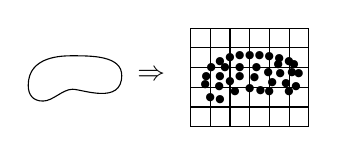
\begin{tikzpicture}[scale=0.25]
  % \draw[step=1.0,black,thin] (-3.,-1.) grid (3,4.);
  % \draw (-3,-1) -- (3,-1) -- (3,4) -- (-3,4) -- (-3,-1);
  \begin{scope}[scale=0.5]
    \draw (-3,0.6) .. controls +(1,0) and +(-1,0) .. (0,1.8)  
    .. controls +(1,0) and +(0,-3) .. (5,3.2) 
    .. controls +(0,2) and +(2,0)  .. (0,5.2) 
    .. controls +(-1,0) and +(0,3) .. (-4.5,2.2) 
    .. controls +(0,-1) and +(-1,0).. (-3,0.6) ;
    \begin{scope}  % pour limiter la portée du clip
      \clip (-3,0.6) .. controls +(1,0) and +(-1,0) .. (0,1.8) 
      .. controls +(1,0) and +(0,-3) .. (5,3.2)
      .. controls +(0,2) and +(2,0)  .. (0,5.2)
      .. controls +(-1,0) and +(0,3) .. (-4.5,2.2)
      .. controls +(0,-1) and +(-1,0).. (-3,0.6);
    \end{scope}
    %\node[below] at (0,1) {$\Omega$};
  \end{scope}
  \node at (4.,1.62) {$\Rightarrow$};
  \begin{scope}[shift={(9,0)}]
    \draw[step=1.0,black,thin] (-3.,-1.) grid (3,4.);
    % contour
    \node at (0,0.9) {\scriptsize$\bullet$}  ;
    \node at (2.5,1.65) {\scriptsize$\bullet$}  ; 
    \node at (0,2.6) {\scriptsize$\bullet$}  ;
    \node at (-2.25,1.1) {\scriptsize$\bullet$}  ; 
    \node at (-1.5,0.35) {\scriptsize$\bullet$}  ; 
    \node at (-2.,0.45) {\scriptsize$\bullet$} ;
    \node at (-2.2,1.5) {\scriptsize$\bullet$}  ; 
    \node at (-1.5,2.3) {\scriptsize$\bullet$} ; 
    \node at (2.35,1.) {\scriptsize$\bullet$}  ;
    \node at (2.25,2.15) {\scriptsize$\bullet$}  ;
    \node at (0.55,0.8) {\scriptsize$\bullet$}  ; 
    \node at (-0.5,2.6) {\scriptsize$\bullet$};
    \node at (0.5,2.59) {\scriptsize$\bullet$}  ;
    \node at (1.5,2.45) {\scriptsize$\bullet$}  ;
    \node at (1,0.75) {\scriptsize$\bullet$}; 
    \node at (2,0.75) {\scriptsize$\bullet$}  ;
    \node at (2,2.3) {\scriptsize$\bullet$}  ;
    \node at (1,2.55) {\scriptsize$\bullet$}  ;
    \node at (-1,2.5) {\scriptsize$\bullet$}  ; 
    \node at (-1.95,2.) {\scriptsize$\bullet$}  ;
    % interior
    \node at (-1.5,1.5) {\scriptsize$\bullet$}  ; 
    \node at (-1.25,2.) {\scriptsize$\bullet$}  ;
    \node at (-0.75,0.75) {\scriptsize$\bullet$}  ; 
    \node at (-1.55,1.){\scriptsize$\bullet$} ;
    \node at (-0.5,1.5) {\scriptsize$\bullet$}  ; 
    \node at (-0.5,2.) {\scriptsize$\bullet$}  ;
    \node at (0.25,1.45) {\scriptsize$\bullet$}  ;
    \node at (0.35,2.) {\scriptsize$\bullet$}  ;
    \node at (0.95,1.75) {\scriptsize$\bullet$}  ;
    \node at (1.15,1.2) {\scriptsize$\bullet$} ;
    \node at (1.45,2.15) {\scriptsize$\bullet$}  ; 
    \node at (1.55,1.65) {\scriptsize$\bullet$}  ;
    \node at (1.85,1.15) {\scriptsize$\bullet$}  ; 
    \node at (2.15,1.75) {\scriptsize$\bullet$}  ;
    \node at (-1.,1.25) {\scriptsize$\bullet$}  ;
    % \draw(3,0.5) -- (3.4,0.5) node [right]  {$\Omega_g$};
  \end{scope}
\end{tikzpicture}

%%% Local Variables:
%%% mode: latex
%%% TeX-master: "../presentation"
%%% End:
}
  {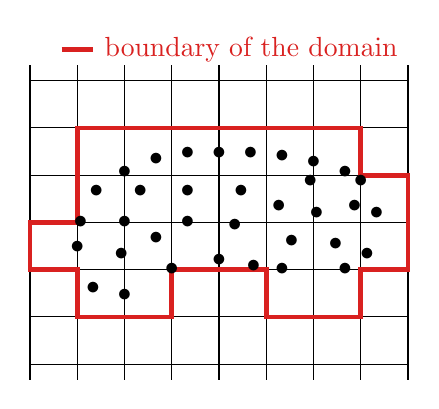
\begin{tikzpicture}[scale=0.8]
  \draw[step=.75,black,thin] (-3.,-1.) grid (3,4.);
  \draw[line width=0.6mm,Red] (-2.25,2.25) -- (-2.25,2.25)-- (-2.25,3)-- (2.25,3) --(2.25,2.25) -- (3.,2.25)-- (3.,0.75) --(2.25,0.75) --(2.25,0.) -- (0.75,0.) --(0.75,0.75) --(-0.75,0.75)-- (-0.75,0.)-- (-2.25,0.) -- (-2.25,0.75) --  (-3.,0.75)--(-3.,1.5) --(-2.25,1.5)--(-2.25,2.25);
  % contour
  \node at (0,0.9) {$\bullet$}  ; \node at (2.5,1.65) {$\bullet$}  ; 
  \node at (0,2.6) {$\bullet$}  ;\node at (-2.25,1.1) {$\bullet$}  ; 
  \node at (-1.5,0.35) {$\bullet$}  ; \node at (-2.,0.45) {$\bullet$}  ;
  \node at (-2.2,1.5) {$\bullet$}  ; \node at (-1.5,2.3) {$\bullet$}  ; 
  \node at (2.35,1.) {$\bullet$}  ; \node at (2.25,2.15) {$\bullet$}  ;
  \node at (0.55,0.8) {$\bullet$}  ; \node at (-0.5,2.6) {$\bullet$}  ; 
  \node at (0.5,2.59) {$\bullet$}  ; \node at (1.5,2.45) {$\bullet$}  ;
  \node at (1,0.75) {$\bullet$}; \node at (2,0.75) {$\bullet$}  ;
  \node at (2,2.3) {$\bullet$}  ; \node at (1,2.55) {$\bullet$}  ;
  \node at (-1,2.5) {$\bullet$}  ; \node at (-1.95,2.) {$\bullet$}  ;
  % interior
  \node at (-1.5,1.5) {$\bullet$}  ; \node at (-1.25,2.) {$\bullet$}  ;
  \node at (-0.75,0.75) {$\bullet$}  ; \node at (-1.55,1.) {$\bullet$}  ;
  \node at (-0.5,1.5) {$\bullet$}  ; \node at (-0.5,2.) {$\bullet$}  ;
  \node at (0.25,1.45) {$\bullet$}  ; \node at (0.35,2.) {$\bullet$}  ;
  \node at (0.95,1.75) {$\bullet$}  ; \node at (1.15,1.2) {$\bullet$}  ;
  \node at (1.45,2.15) {$\bullet$}  ; \node at (1.55,1.65) {$\bullet$}  ;
  \node at (1.85,1.15) {$\bullet$}  ; \node at (2.15,1.75) {$\bullet$}  ;
  \node at (-1.,1.25) {$\bullet$}  ;
  \draw[line width=0.6mm,Red] (-2.5,4.25) -- (-2.,4.25) node [right] {\text{boundary of the domain}};
\end{tikzpicture}}
  \caption{Representation of a continuum body by a set of material points in $\Rbb^2$.}
  \label{fig:domain}	
\end{figure}
Analogously to the Finite Element Method (FEM) \cite{Belytschko}, the velocity is approximated on the MPM background mesh by:
\begin{equation}
  \label{eq:approximation_basis}
  \vect{v}(\vect{x},t)=S_i(\vect{x})\vect{v}^{i}(t)
\end{equation}
where $\vect{v}^{i}$ is the velocity of the $i$th grid node, and $S_i(\vect{x})$ the (linear) shape function attached to it. One feature of the MPM is that the mass density is approximated on the grid based on the mass carried by each material point:
\begin{equation}
  \label{eq:density_approx}
  \rho\(\vect{x},t\)=\sum_{p=1}^{N_p} m_p \delta(\vect{x}_p-\vect{x})
\end{equation}
where the delta Dirac distribution $\delta$ is often referred to as the \textit{characteristic function} of material points, and $\vect{x}_p$ is the position of the $p$th particle. In what follows, the dependence on time will be omitted for simplicity and $p$ and $i$ or $j$ stand respectively for material points and nodes.

By introducing a specific Cauchy tensor $\rho \tens{\bar{\sigma}}=\tens{\sigma}$ and the approximation of mass density \eqref{eq:density_approx} in the weak form \eqref{eq:linear_momentum_weak_form}, the property of the delta Dirac distribution yields:
\begin{equation}
  \begin{aligned}
    &\text{Find $\vect{v}\in \Vscr_h^1$ such that} \\
    & \sum_{p=1}^{N_p} m_p  \[\vect{\dot{v}}(\vect{x}_p) \cdot \vect{w}(\vect{x}_p) + \tens{\bar{\sigma}}(\vect{x}_p):\nablat \vect{w}(\vect{x}_p) \]  = \sum_{p=1}^{N_p}m_p \vect{b}(\vect{x}_p)\cdot \vect{w}(\vect{x}_p) + \int_{\partial \Omega^\sigma_t} \vect{T}^d\cdot\vect{w}\: ds  \qquad \forall \: \vect{w} \in \Vscr_{h,0}^1
  \end{aligned}
\end{equation}
Then, with the approximation \eqref{eq:approximation_basis}, the weak form reads:
\begin{equation}
  \label{eq:mpm_discrete_weak}
    \begin{aligned}
      &\text{Find $\vect{v} \in \Vscr_h^1$ such that} \\
      & \vect{w}^j \sum_{p=1}^{N_p} m_p  \[ S_{jp} S_{ip} \vect{\dot{v}}^i + \nablav S_{jp} \cdot \tens{\bar{\sigma}}^p \]  =  \vect{w}^j\( \sum_{p=1}^{N_p}m_p S_{jp}\vect{b}^i  + \int_{\partial \Omega^\sigma_t} S_j(\vect{x})\vect{T}^d\: ds\)  \qquad \forall \: \vect{w} \in \Vscr_{h,0}^1
  \end{aligned}
\end{equation}
in which $S_{ip}=S_i(\vect{x}_p)$ and $\tens{\bar{\sigma}}^p=\tens{\bar{\sigma}}(\vect{x}_p)$. Next, the arbitrariness of the test function $\vect{w}$ yields the semi-discrete equation in matrix form:
\begin{equation}
  \label{eq:mpm_semi-discrete}
  m_{ji} \vect{\dot{v}}^i = \vect{f}_{int}^j + \vect{f}_{ext}^j 
\end{equation}
where the definition of the mass matrix $m_{ij}$ and the internal and external force vectors $\vect{f}_{int}^j $ and $\vect{f}_{ext}^j$ are:
\begin{subequations}
  \begin{alignat}{1}
    & m_{ij}= \sum_{p=1}^{N_p} m_p  S_{jp} S_{ip} \label{eq:mass_matrix}\\
    & \vect{f}_{int}^j = - \sum_{p=1}^{N_p} m_p \nablav S_{jp} \cdot \tens{\bar{\sigma}}^p \label{eq:int_forces}\\
    & \vect{f}_{ext}^j =\sum_{p=1}^{N_p}m_p S_{jp}\vect{b}^i  + \int_{\partial \Omega^\sigma_t} S_j(\vect{x})\vect{T}^d\: ds \label{eq:ext_forces}
  \end{alignat}
\end{subequations}
The system \eqref{eq:mpm_semi-discrete} can be solved for the nodal accelerations $\vect{\dot{v}}^i$, and advanced in time by using an explicit time discretization so that the nodal velocities can be updated. Hence, the time interval $\tau$ is discretized in $N_T$ sub-intervals of size $\Delta t^n$ such that $\sum_{n=1}^{N_T} \Delta t^n = T$ and time integration is performed with an explicit forward Euler algorithm leading to discrete equations:
\begin{equation}
  \label{eq:mpm_discrete}
  \frac{\vect{v}^{i,n+1}-\vect{v}^{i,n}}{\Delta t^n} = \vect{\dot{v}}^i
\end{equation}
where the superscripts $\bullet^{k,l}$ denote the time step $l$ at which the $k$th nodal field is evaluated. 

Note that in the weak form, the particles play the role of integration points so that the mass matrix depends on the positions of material points in the grid and must be computed at each time step. Hence, the MPM can be seen as an extension of the Finite Element Method with moving Gauss points. However, a consequence of this quadrature rule is that the consistent mass matrix $m_{ji}$ may be singular when only one material point lies in an element due to the reduced integration. The use of a linear combination of the diagonally lumped mass matrix $m^L_i=\sum_p S_{ip}m_p$ (positive-definite), and the constitent mass matrix (positive semi-definite) is then recommended \cite{Love}. Nevertheless, since no parameter value is prescribed for this combination, the lumped mass matrix is widely used in MPM simulations, though it introduces some dissipation of kinetic energy \cite{Mass_Flip}.  

Recall that the background grid inherited from FLIP is arbitrary and that the fields must be projected from particles to the nodes to solve the linear system \eqref{eq:mpm_discrete} and back so that the material points advect the solution. The first mapping step, required to build the discrete form,
aims at satify the conservation of linear momentum from particles to the grid:
\begin{equation}
  \label{eq:particles2nodes}
  m^{L,n}_i \vect{v}^{i,n} = \sum_{p=1}^{N_p} S_{ip}m_p \vect{v}^{p,n}
\end{equation}
to be solved for each $\vect{v}^i$. Once the nodal accelerations are calculeted for system \eqref{eq:mpm_semi-discrete}, the velocity of each material points is \textbf{updated} as:
\begin{equation}
  \label{eq:mp_velocity_update}
  \vect{v}^{p,n+1}= \vect{v}^{p,n}+ \Delta t\sum_{i=1}^{N_n} S_{ip}\vect{\dot{v}}^{i}
\end{equation}
while the updated nodal velocities resulting from the solution of \eqref{eq:mpm_discrete} are used to update the particles positions:
\begin{equation}
  \label{eq:position_update}
  \vect{x}^{p,n+1}=\vect{x}^{p,n} + \Delta t\sum_{i=1}^{N_n} S_{ip}\vect{v}^{i,n+1} 
\end{equation}

The integration of constitutive equations is performed at material points based on the nodal velocity field and the gradient of shape functions. Hence, one has some freedom in the way in which the stress is computed since it can be done right after either the resolution of \eqref{eq:mpm_discrete} or the projection \eqref{eq:particles2nodes}. The first option yields the \textit{Update Stress Last} (USL) algorithm while the second implementation is called \textit{Update Stress First} (USF) \cite{Bardenhagen_USF_USL}. 

The solution of discrete equations on the background grid requires the enforcement of boundary conditions at nodes. While Neumann boundary conditions are prescribed through the external force vector (equation \eqref{eq:ext_forces}), Dirichlet boundary conditions have to be imposed on both nodal acceleration and velocity in order to consistently update the kinematics and constitutive equations at material points. The enforcement of boundary condition is still a chalenging aspect of the material point method (as others mesh-free methods) for problems involving complex geometries, see for instance \cite{Bcs_MPM}. However, we consider here problems that do not require a particular treatment of boundary conditions.

\subsubsection{Solution scheme summary}
Let us assume that position and velocity vectors  $\vect{x}^n$ and $\vect{v}^n$ are known at every material points that discretize the continuum body in the grid at time $t^n$. Moreover, the USL implementation of the method also requires the knowledge of the specific stress tensor $\tens{\bar{\sigma}}^n$ at material points. The MPM solution scheme then consists of the following steps:
\begin{itemize}
\item[(a)] Computation of the consistent and lumped mass matrices and external forces (Neumann boundary conditions) from equations \eqref{eq:mass_matrix} and \eqref{eq:ext_forces}.
\item[(b)] Convective phase: projection of fields to the grid \eqref{eq:particles2nodes} and enforce Dirichlet boundary conditions on the nodal velocity. For USF formulation, the enforcement of Dirichlet boundary conditions on the mesh is required so that the integration of constitutive equations can be done.
\item[(c)] Evaluation of internal forces from equation \eqref{eq:int_forces}.
\item[(d)] Solution of the semi-discrete and discrete forms \eqref{eq:mpm_semi-discrete} and \eqref{eq:mpm_discrete} so that nodal accelerations $\vect{\dot{v}}^i$ and updated velocities $\vect{v}^{i,n+1}$ are determined. Enforcement of Dirichlet boundary conditions: set the velocity of boundary nodes to the prescribed values and their accelerations to zero.
\item[(e)] Update the material points velocities and positions with equations \eqref{eq:mp_velocity_update} and \eqref{eq:position_update} respectively. At this point the mesh has virtually moved, but since fields have been transferred back to particles, the underlying grid can be discarded and rebuilt for the next time step for computational convenience, thus involving the convective phase (b) at the next time step. 
\item[(f)] If the USL implementation is set, constitutive equations must be integrated.
\end{itemize}

Although the material point method has been successfully applied to a wide range of complex large strain engineering problems involving finite deformations \cite{Wieckowski}, this approach suffers from limitations which are discussed in the next section. 

\subsection{Shortcomings of the MPM}

%% Quick way
%The computation of internal forces within the MPM may lead to the well-known \textit{grid-crossing} instability due to the discontinuity of the gradient of shape functions when material points move from one cell to another \cite{Gimp}. The \textbf{Generalized Interpolation Material Point method} (GIMP) \cite{Gimp}, the \textbf{B-Spline Material Point Method} (BSMPM) \cite{Steffen_quadError} and the \textbf{Dual Domain Material Point Method} (DDMPM) \cite{DDMPM0} addressed this issue respectively by: (i) changing the particles characteristic function; (ii) enriching the approximation basis with quadratic or cubic B-Spline functions; (iii) introducing a modified gradient of shape functions. 

\subsubsection*{The grid-crossing instability}
The research on MPM mainly focused so far on the instability arising from the computation of internal forces when material points move from one cell to another due to the discontinuity of the gradient of shape functions across element interfaces, the so-called \textit{grid-crossing} error \cite{Gimp}. The \textbf{Generalized Interpolation Material Point Method} (GIMP) addressed this numerical issue by modifying the particles characteristic function, thus widening the domain of influence of material points \cite{Gimp}. By doing so, every particle are given a domain having either a constant shape (the uGIMP formulation) or not (the cpGIMP formulation), that must be tracked during the computation. In the cpGimp algorithm, only diagonal entries of the deformation gradient are used to update the "shapes" of particles. The \textbf{Convected Particle Domain Interpolation} (CPDI) \cite{CPDI} has then been developed to account for shear deformations an rotations of particles domains, thus providing an improvement of GIMP. However, those methods involve other difficulties related to the tracking of the deforming domains material points in the Eulerian grid which leads to mesh entanglement issues \cite{DDMPM0}. As a consequence, other ways consisting in the direct modification of the approximation basis have been followed to tackle the grid-crossing error. First, the \textbf{B-Spline Material Point Method} (BSMPM) \cite{Steffen_quadError} uses quadratic or cubic B-Spline functions with continuous gradients as nodal shape functions which allow to circumvent the instability \cite{MPM_BSpline1}. Second, the classical approximation basis is used and modified gradients with extended supports are introduced in the \textbf{Dual Domain Material Point Method} (DDMPM) \cite{DDMPM0}. These approaches both solve the grid-crossing error by widening the domain of influence of material points since B-Spline functions span more cells than Lagrange polynomials and the supports of the modified gradients of the DDMPM are larger than those of the shape functions.  

\subsubsection*{The back-mapping instability}
Numerical noise also appears in the MPM solution for problems that do not involve the grid-crossing instability. As an illustration of the previous remark, let us consider a one-dimensional elastic bar of length $L=6\:m$ with Young's modulus $E=200 \:GPa$ and mass density $\rho=7800 \:kg\cdot m^{-3}$ within the infinitesimal theory. The bar is initially in a free stress state and Riemann-type initial velocities are prescribed along the bar, that is: $v=v_0>0$ for $x\in[0,L/2]$ and $v=-v_0$ for $x \in [L/2,L]$. Both ends of the bar are traction free so that this problem is equivalent to an impact of two elastic bars moving toward each other. The analytical solution of this problem (see section \ref{subsec:charac_Linear_problems}) consists of two elastic discontinuities emanating from the middle of the bar and propagating left and rightward. Numerical results provided by the USL and USF implementations of the MPM are compared to the exact solution before reflection of the waves on the boundaries in figure \ref{fig:US_diffusion}. The computational grid is composed of $50$ regular cells, each containing either one or two material points ($1\: ppc$ or $2\: ppc$). Single material points are centered in cells while "cellmate" particles are placed symmetrically with respect to elements centers and are regularly spaced. 
\begin{figure}[h!]
  \centering
  {\definecolor{Purple}{RGB}{120,28,129}
\definecolor{Orange}{RGB}{231,133,50}
\definecolor{Blue}{RGB}{63,96,174}
\definecolor{Red}{RGB}{217,33,32}
\definecolor{Duck}{RGB}{83,158,182}
\definecolor{Green}{RGB}{109,179,136}
\definecolor{Yellow}{RGB}{202,184,67}
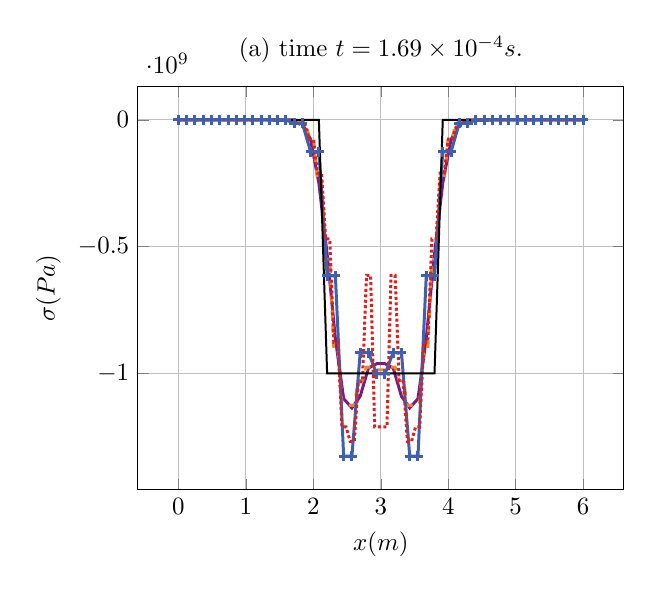
\begin{tikzpicture}[scale=0.9]
\begin{axis}[xlabel=$x (m)$,ylabel=$\sigma (Pa)$,ymajorgrids=true,xmajorgrids=true,title={(a) time $t =1.69\times 10^{-4}s.$}]
\addplot[Purple,very thick,mark=none,solid] coordinates {(0.0,-9.62200780097e-08) (0.122448979592,-1.92440156019e-07) (0.244897959184,-9.62200780097e-08) (0.367346938776,0.0) (0.489795918367,9.62200780097e-08) (0.612244897959,-9.62200780097e-08) (0.734693877551,-1.92440156019e-07) (0.857142857143,-9.62200780097e-08) (0.979591836735,-9.62200780097e-08) (1.10204081633,0.0) (1.22448979592,9.62200780097e-08) (1.34693877551,-9.62200780097e-08) (1.4693877551,0.0) (1.59183673469,0.0) (1.71428571429,0.0) (1.83673469388,-15437652.4848) (1.95918367347,-78183137.9185) (2.08163265306,-249067223.585) (2.20408163265,-529536815.675) (2.32653061224,-862202048.46) (2.44897959184,-1099498863.41) (2.57142857143,-1135789315.44) (2.69387755102,-1090007223.73) (2.81632653061,-978780358.738) (2.9387755102,-961497360.562) (3.0612244898,-961497360.562) (3.18367346939,-978780358.738) (3.30612244898,-1090007223.73) (3.42857142857,-1135789315.44) (3.55102040816,-1099498863.41) (3.67346938776,-862202048.46) (3.79591836735,-529536815.675) (3.91836734694,-249067223.585) (4.04081632653,-78183137.9185) (4.16326530612,-15437652.4848) (4.28571428571,-3.85185988877e-23) (4.40816326531,-9.62200780097e-08) (4.5306122449,9.62200780097e-08) (4.65306122449,9.62200780097e-08) (4.77551020408,9.62200780097e-08) (4.89795918367,-2.88660234029e-07) (5.02040816327,-9.62200780097e-08) (5.14285714286,9.62200780097e-08) (5.26530612245,1.92440156019e-07) (5.38775510204,2.88660234029e-07) (5.51020408163,9.62200780097e-08) (5.63265306122,0.0) (5.75510204082,0.0) (5.87755102041,0.0) (6.0,-9.62200780097e-08) };
\addplot[Orange,very thick,mark=none,dashed] coordinates {(0.0,0.0) (0.0606060606061,0.0) (0.121212121212,9.52481580298e-08) (0.181818181818,9.52481580298e-08) (0.242424242424,9.52481580298e-08) (0.30303030303,9.52481580298e-08) (0.363636363636,0.0) (0.424242424242,0.0) (0.484848484848,-9.52481580298e-08) (0.545454545455,-9.52481580298e-08) (0.606060606061,-1.9049631606e-07) (0.666666666667,-1.9049631606e-07) (0.727272727273,0.0) (0.787878787879,0.0) (0.848484848485,0.0) (0.909090909091,0.0) (0.969696969697,-3.85185988877e-23) (1.0303030303,-3.85185988877e-23) (1.09090909091,-9.52481580298e-08) (1.15151515152,-9.52481580298e-08) (1.21212121212,9.52481580298e-08) (1.27272727273,9.52481580298e-08) (1.33333333333,9.52481580298e-08) (1.39393939394,9.52481580298e-08) (1.45454545455,-1.9049631606e-07) (1.51515151515,-1.9049631606e-07) (1.57575757576,1.9049631606e-07) (1.63636363636,1.9049631606e-07) (1.69696969697,0.0) (1.75757575758,0.0) (1.81818181818,-9533923.2537) (1.87878787879,-9533923.2537) (1.93939393939,-67166647.336) (2.0,-67166647.336) (2.06060606061,-239339979.822) (2.12121212121,-239339979.822) (2.18181818182,-549695480.518) (2.24242424242,-549695480.518) (2.30303030303,-900240202.504) (2.36363636364,-900240202.504) (2.42424242424,-1118552245.0) (2.48484848485,-1118552245.0) (2.54545454545,-1125362633.2) (2.60606060606,-1125362633.2) (2.66666666667,-1028724363.35) (2.72727272727,-1028724363.35) (2.78787878788,-975375246.836) (2.84848484848,-975375246.836) (2.90909090909,-986009278.185) (2.9696969697,-986009278.185) (3.0303030303,-986009278.185) (3.09090909091,-986009278.185) (3.15151515152,-975375246.836) (3.21212121212,-975375246.836) (3.27272727273,-1028724363.35) (3.33333333333,-1028724363.35) (3.39393939394,-1125362633.2) (3.45454545455,-1125362633.2) (3.51515151515,-1118552245.0) (3.57575757576,-1118552245.0) (3.63636363636,-900240202.504) (3.69696969697,-900240202.504) (3.75757575758,-549695480.518) (3.81818181818,-549695480.518) (3.87878787879,-239339979.822) (3.93939393939,-239339979.822) (4.0,-67166647.336) (4.06060606061,-67166647.336) (4.12121212121,-9533923.2537) (4.18181818182,-9533923.2537) (4.24242424242,9.52481580298e-08) (4.30303030303,9.52481580298e-08) (4.36363636364,-9.52481580298e-08) (4.42424242424,-9.52481580298e-08) (4.48484848485,0.0) (4.54545454545,0.0) (4.60606060606,0.0) (4.66666666667,0.0) (4.72727272727,0.0) (4.78787878788,0.0) (4.84848484848,0.0) (4.90909090909,0.0) (4.9696969697,0.0) (5.0303030303,0.0) (5.09090909091,0.0) (5.15151515152,0.0) (5.21212121212,0.0) (5.27272727273,0.0) (5.33333333333,0.0) (5.39393939394,0.0) (5.45454545455,0.0) (5.51515151515,0.0) (5.57575757576,0.0) (5.63636363636,0.0) (5.69696969697,0.0) (5.75757575758,0.0) (5.81818181818,0.0) (5.87878787879,0.0) (5.93939393939,9.52481580298e-08) (6.0,9.52481580298e-08) };
\addplot[Blue,very thick,mark=+,solid] coordinates {(0.0,-3.84880312039e-07) (0.122448979592,2.88660234029e-07) (0.244897959184,-5.77320468058e-07) (0.367346938776,2.88660234029e-07) (0.489795918367,-9.62200780097e-08) (0.612244897959,2.88660234029e-07) (0.734693877551,-4.3483336004) (0.857142857143,-4.34833340796) (0.979591836735,-560.668787915) (1.10204081633,-560.668788299) (1.22448979592,-29850.7439455) (1.34693877551,-29850.7439456) (1.4693877551,-846060.279927) (1.59183673469,-846060.279927) (1.71428571429,-13703737.6015) (1.83673469388,-13703737.6015) (1.95918367347,-126206739.753) (2.08163265306,-126206739.753) (2.20408163265,-614922268.389) (2.32653061224,-614922268.389) (2.44897959184,-1325731906.52) (2.57142857143,-1325731906.52) (2.69387755102,-917663590.795) (2.81632653061,-917663590.795) (2.9387755102,-1001790561.8) (3.0612244898,-1001790561.8) (3.18367346939,-917663590.795) (3.30612244898,-917663590.795) (3.42857142857,-1325731906.52) (3.55102040816,-1325731906.52) (3.67346938776,-614922268.389) (3.79591836735,-614922268.389) (3.91836734694,-126206739.753) (4.04081632653,-126206739.753) (4.16326530612,-13703737.6015) (4.28571428571,-13703737.6015) (4.40816326531,-846060.279927) (4.5306122449,-846060.279927) (4.65306122449,-29850.7439458) (4.77551020408,-29850.7439452) (4.89795918367,-560.668787818) (5.02040816327,-560.668788011) (5.14285714286,-4.34833331174) (5.26530612245,-4.34833340796) (5.38775510204,1.92440156019e-07) (5.51020408163,-9.62200780097e-08) (5.63265306122,1.92440156019e-07) (5.75510204082,-2.88660234029e-07) (5.87755102041,4.81100390048e-07) (6.0,-2.88660234029e-07) };
\addplot[Red,very thick,mark=none,densely dotted] coordinates {(0.0,0.0) (0.0606060606061,0.0) (0.121212121212,9.52481580298e-08) (0.181818181818,9.52481580298e-08) (0.242424242424,-7.70371977755e-23) (0.30303030303,-7.70371977755e-23) (0.363636363636,-9.52481580298e-08) (0.424242424242,-9.52481580298e-08) (0.484848484848,-1.9049631606e-07) (0.545454545455,-1.9049631606e-07) (0.606060606061,1.9049631606e-07) (0.666666666667,1.9049631606e-07) (0.727272727273,-0.326493160065) (0.787878787879,-0.326493160065) (0.848484848485,-4.24441250957) (0.909090909091,-4.24441250957) (0.969696969697,-75.0667952395) (1.0303030303,-75.0667952395) (1.09090909091,-676.110516968) (1.15151515152,-676.110516968) (1.21212121212,-6409.50756423) (1.27272727273,-6409.50756423) (1.33333333333,-42608.4474487) (1.39393939394,-42608.4474487) (1.45454545455,-271096.202803) (1.51515151515,-271096.202803) (1.57575757576,-1361323.47494) (1.63636363636,-1361323.47494) (1.69696969697,-6186277.73843) (1.75757575758,-6186277.73843) (1.81818181818,-23394049.9045) (1.87878787879,-23394049.9045) (1.93939393939,-76154273.8888) (2.0,-76154273.8888) (2.06060606061,-210327688.316) (2.12121212121,-210327688.316) (2.18181818182,-469773248.386) (2.24242424242,-469773248.386) (2.30303030303,-877374801.132) (2.36363636364,-877374801.132) (2.42424242424,-1211041212.86) (2.48484848485,-1211041212.86) (2.54545454545,-1267995558.57) (2.60606060606,-1267995558.57) (2.66666666667,-1032834595.27) (2.72727272727,-1032834595.27) (2.78787878788,-612908579.142) (2.84848484848,-612908579.142) (2.90909090909,-1210327521.41) (2.9696969697,-1210327521.41) (3.0303030303,-1210327521.41) (3.09090909091,-1210327521.41) (3.15151515152,-612908579.142) (3.21212121212,-612908579.142) (3.27272727273,-1032834595.27) (3.33333333333,-1032834595.27) (3.39393939394,-1267995558.57) (3.45454545455,-1267995558.57) (3.51515151515,-1211041212.86) (3.57575757576,-1211041212.86) (3.63636363636,-877374801.132) (3.69696969697,-877374801.132) (3.75757575758,-469773248.386) (3.81818181818,-469773248.386) (3.87878787879,-210327688.316) (3.93939393939,-210327688.316) (4.0,-76154273.8888) (4.06060606061,-76154273.8888) (4.12121212121,-23394049.9045) (4.18181818182,-23394049.9045) (4.24242424242,-6186277.73843) (4.30303030303,-6186277.73843) (4.36363636364,-1361323.47494) (4.42424242424,-1361323.47494) (4.48484848485,-271096.202803) (4.54545454545,-271096.202803) (4.60606060606,-42608.4474489) (4.66666666667,-42608.4474489) (4.72727272727,-6409.50756433) (4.78787878788,-6409.50756433) (4.84848484848,-676.110516873) (4.90909090909,-676.110516873) (4.9696969697,-75.0667953347) (5.0303030303,-75.0667953347) (5.09090909091,-4.24441231907) (5.15151515152,-4.24441231907) (5.21212121212,-0.326493255313) (5.27272727273,-0.326493255313) (5.33333333333,0.0) (5.39393939394,0.0) (5.45454545455,0.0) (5.51515151515,0.0) (5.57575757576,0.0) (5.63636363636,0.0) (5.69696969697,0.0) (5.75757575758,0.0) (5.81818181818,0.0) (5.87878787879,0.0) (5.93939393939,0.0) (6.0,0.0) };
\addplot[black,thick] coordinates {(0.0,-0.0) (0.122448979592,-0.0) (0.244897959184,-0.0) (0.367346938776,-0.0) (0.489795918367,-0.0) (0.612244897959,-0.0) (0.734693877551,-0.0) (0.857142857143,-0.0) (0.979591836735,-0.0) (1.10204081633,-0.0) (1.22448979592,-0.0) (1.34693877551,-0.0) (1.4693877551,-0.0) (1.59183673469,-0.0) (1.71428571429,-0.0) (1.83673469388,-0.0) (1.95918367347,-0.0) (2.08163265306,-0.0) (2.20408163265,-1000000000.0) (2.32653061224,-1000000000.0) (2.44897959184,-1000000000.0) (2.57142857143,-1000000000.0) (2.69387755102,-1000000000.0) (2.81632653061,-1000000000.0) (2.9387755102,-1000000000.0) (3.0612244898,-1000000000.0) (3.18367346939,-1000000000.0) (3.30612244898,-1000000000.0) (3.42857142857,-1000000000.0) (3.55102040816,-1000000000.0) (3.67346938776,-1000000000.0) (3.79591836735,-1000000000.0) (3.91836734694,-0.0) (4.04081632653,-0.0) (4.16326530612,-0.0) (4.28571428571,-0.0) (4.40816326531,-0.0) (4.5306122449,-0.0) (4.65306122449,-0.0) (4.77551020408,-0.0) (4.89795918367,-0.0) (5.02040816327,-0.0) (5.14285714286,-0.0) (5.26530612245,-0.0) (5.38775510204,-0.0) (5.51020408163,-0.0) (5.63265306122,-0.0) (5.75510204082,-0.0) (5.87755102041,-0.0) (6.0,-0.0) };
%\legend{USL 1ppc,USL 2ppc,USF 1ppc,USF 2ppc}
\end{axis}
\end{tikzpicture}
 \phantomsubcaption \label{subfig:US_diffusion_10}}
  {\definecolor{Purple}{RGB}{120,28,129}
\definecolor{Orange}{RGB}{231,133,50}
\definecolor{Blue}{RGB}{63,96,174}
\definecolor{Red}{RGB}{217,33,32}
\definecolor{Duck}{RGB}{83,158,182}
\definecolor{Green}{RGB}{109,179,136}
\definecolor{Yellow}{RGB}{202,184,67}
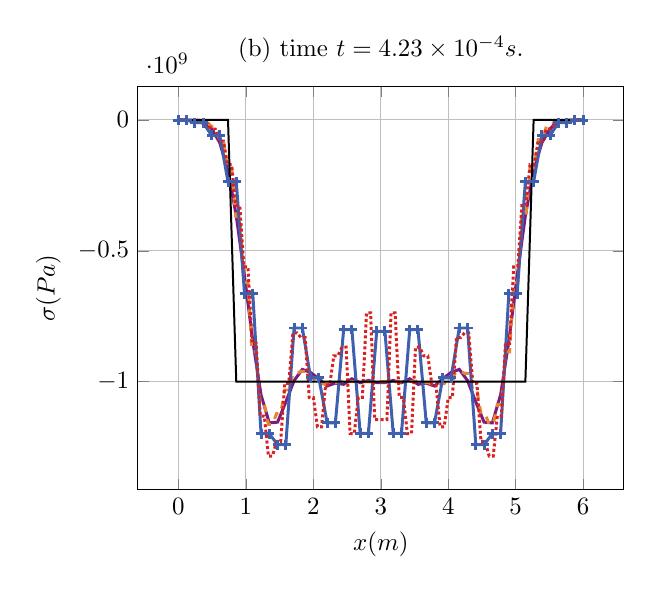
\begin{tikzpicture}[scale=0.9]
\begin{axis}[xlabel=$x (m)$,ylabel=$\sigma (Pa)$,ymajorgrids=true,xmajorgrids=true,title={(b) time $t= 4.23\times 10^{-4}s.$}]
\addplot[Purple,very thick,mark=none,solid] coordinates {(0.0,-39934.2174897) (0.122448979592,-406302.064953) (0.244897959184,-2420460.88495) (0.367346938776,-10136844.8366) (0.489795918367,-33063216.5915) (0.612244897959,-87547121.3685) (0.734693877551,-194171704.565) (0.857142857143,-366493404.576) (0.979591836735,-596875114.898) (1.10204081633,-845116689.368) (1.22448979592,-1050481005.19) (1.34693877551,-1157297307.0) (1.4693877551,-1154376682.02) (1.59183673469,-1077374033.62) (1.71428571429,-995689036.388) (1.83673469388,-952936697.469) (1.95918367347,-964832377.273) (2.08163265306,-988568067.368) (2.20408163265,-1016260759.09) (2.32653061224,-1005179173.62) (2.44897959184,-1009892551.13) (2.57142857143,-988773783.034) (2.69387755102,-1003829596.99) (2.81632653061,-995025027.704) (2.9387755102,-1003213108.71) (3.0612244898,-1003213108.71) (3.18367346939,-995025027.704) (3.30612244898,-1003829596.99) (3.42857142857,-988773783.034) (3.55102040816,-1009892551.13) (3.67346938776,-1005179173.62) (3.79591836735,-1016260759.09) (3.91836734694,-988568067.368) (4.04081632653,-964832377.273) (4.16326530612,-952936697.469) (4.28571428571,-995689036.388) (4.40816326531,-1077374033.62) (4.5306122449,-1154376682.02) (4.65306122449,-1157297307.0) (4.77551020408,-1050481005.19) (4.89795918367,-845116689.368) (5.02040816327,-596875114.898) (5.14285714286,-366493404.576) (5.26530612245,-194171704.565) (5.38775510204,-87547121.3685) (5.51020408163,-33063216.5915) (5.63265306122,-10136844.8366) (5.75510204082,-2420460.88495) (5.87755102041,-406302.064953) (6.0,-39934.2174897) };
\addplot[Orange,very thick,mark=none,dashed] coordinates {(0.0,-10429.0753611) (0.0606060606061,-10429.0753611) (0.121212121212,-161982.808053) (0.181818181818,-161982.808053) (0.242424242424,-1267409.75703) (0.30303030303,-1267409.75703) (0.363636363636,-6575307.60772) (0.424242424242,-6575307.60772) (0.484848484848,-25213047.7874) (0.545454545455,-25213047.7874) (0.606060606061,-75630068.1866) (0.666666666667,-75630068.1866) (0.727272727273,-183565723.323) (0.787878787879,-183565723.323) (0.848484848485,-368376215.18) (0.909090909091,-368376215.18) (0.969696969697,-620238104.743) (1.0303030303,-620238104.743) (1.09090909091,-886041263.042) (1.15151515152,-886041263.042) (1.21212121212,-1086232263.3) (1.27272727273,-1086232263.3) (1.33333333333,-1162610811.08) (1.39393939394,-1162610811.08) (1.45454545455,-1121800356.23) (1.51515151515,-1121800356.23) (1.57575757576,-1031608883.18) (1.63636363636,-1031608883.18) (1.69696969697,-967968470.151) (1.75757575758,-967968470.151) (1.81818181818,-960540680.349) (1.87878787879,-960540680.349) (1.93939393939,-986227377.719) (2.0,-986227377.719) (2.06060606061,-1007602191.25) (2.12121212121,-1007602191.25) (2.18181818182,-1009726046.8) (2.24242424242,-1009726046.8) (2.30303030303,-1002072997.71) (2.36363636364,-1002072997.71) (2.42424242424,-997465464.463) (2.48484848485,-997465464.463) (2.54545454545,-998318352.653) (2.60606060606,-998318352.653) (2.66666666667,-1000280134.99) (2.72727272727,-1000280134.99) (2.78787878788,-1000550813.71) (2.84848484848,-1000550813.71) (2.90909090909,-999915604.91) (2.9696969697,-999915604.91) (3.0303030303,-999915604.91) (3.09090909091,-999915604.91) (3.15151515152,-1000550813.71) (3.21212121212,-1000550813.71) (3.27272727273,-1000280134.99) (3.33333333333,-1000280134.99) (3.39393939394,-998318352.653) (3.45454545455,-998318352.653) (3.51515151515,-997465464.463) (3.57575757576,-997465464.463) (3.63636363636,-1002072997.71) (3.69696969697,-1002072997.71) (3.75757575758,-1009726046.8) (3.81818181818,-1009726046.8) (3.87878787879,-1007602191.25) (3.93939393939,-1007602191.25) (4.0,-986227377.719) (4.06060606061,-986227377.719) (4.12121212121,-960540680.349) (4.18181818182,-960540680.349) (4.24242424242,-967968470.151) (4.30303030303,-967968470.151) (4.36363636364,-1031608883.18) (4.42424242424,-1031608883.18) (4.48484848485,-1121800356.23) (4.54545454545,-1121800356.23) (4.60606060606,-1162610811.08) (4.66666666667,-1162610811.08) (4.72727272727,-1086232263.3) (4.78787878788,-1086232263.3) (4.84848484848,-886041263.042) (4.90909090909,-886041263.042) (4.9696969697,-620238104.743) (5.0303030303,-620238104.743) (5.09090909091,-368376215.18) (5.15151515152,-368376215.18) (5.21212121212,-183565723.323) (5.27272727273,-183565723.323) (5.33333333333,-75630068.1866) (5.39393939394,-75630068.1866) (5.45454545455,-25213047.7874) (5.51515151515,-25213047.7874) (5.57575757576,-6575307.60772) (5.63636363636,-6575307.60772) (5.69696969697,-1267409.75703) (5.75757575758,-1267409.75703) (5.81818181818,-161982.808054) (5.87878787879,-161982.808054) (5.93939393939,-10429.0753609) (6.0,-10429.0753609) };
\addplot[Blue,very thick,mark=+,solid] coordinates {(0.0,-1333876.13913) (0.122448979592,-1333876.13913) (0.244897959184,-10769880.3244) (0.367346938776,-10769880.3244) (0.489795918367,-59004320.4619) (0.612244897959,-59004320.4619) (0.734693877551,-236932522.32) (0.857142857143,-236932522.32) (0.979591836735,-663853517.052) (1.10204081633,-663853517.052) (1.22448979592,-1198320286.6) (1.34693877551,-1198320286.6) (1.4693877551,-1240363116.33) (1.59183673469,-1240363116.33) (1.71428571429,-794840746.96) (1.83673469388,-794840746.96) (1.95918367347,-985342724.542) (2.08163265306,-985342724.542) (2.20408163265,-1157175976.76) (2.32653061224,-1157175976.76) (2.44897959184,-800603512.041) (2.57142857143,-800603512.041) (2.69387755102,-1197082213.94) (2.81632653061,-1197082213.94) (2.9387755102,-808054803.925) (3.0612244898,-808054803.925) (3.18367346939,-1197082213.94) (3.30612244898,-1197082213.94) (3.42857142857,-800603512.041) (3.55102040816,-800603512.041) (3.67346938776,-1157175976.76) (3.79591836735,-1157175976.76) (3.91836734694,-985342724.542) (4.04081632653,-985342724.542) (4.16326530612,-794840746.96) (4.28571428571,-794840746.96) (4.40816326531,-1240363116.33) (4.5306122449,-1240363116.33) (4.65306122449,-1198320286.6) (4.77551020408,-1198320286.6) (4.89795918367,-663853517.052) (5.02040816327,-663853517.052) (5.14285714286,-236932522.32) (5.26530612245,-236932522.32) (5.38775510204,-59004320.4619) (5.51020408163,-59004320.4619) (5.63265306122,-10769880.3244) (5.75510204082,-10769880.3244) (5.87755102041,-1333876.13913) (6.0,-1333876.13913) };
\addplot[Red,very thick,mark=none,densely dotted] coordinates {(0.0,-388790.247817) (0.0606060606061,-388790.247817) (0.121212121212,-1698682.9889) (0.181818181818,-1698682.9889) (0.242424242424,-5114933.57998) (0.30303030303,-5114933.57998) (0.363636363636,-13968295.6879) (0.424242424242,-13968295.6879) (0.484848484848,-35149039.2515) (0.545454545455,-35149039.2515) (0.606060606061,-81229883.7541) (0.666666666667,-81229883.7541) (0.727272727273,-171384180.27) (0.787878787879,-171384180.27) (0.848484848485,-327574181.976) (0.909090909091,-327574181.976) (0.969696969697,-561694256.942) (1.0303030303,-561694256.942) (1.09090909091,-853480052.942) (1.15151515152,-853480052.942) (1.21212121212,-1131013878.06) (1.27272727273,-1131013878.06) (1.33333333333,-1283904880.31) (1.39393939394,-1283904880.31) (1.45454545455,-1228113384.33) (1.51515151515,-1228113384.33) (1.57575757576,-1005886402.14) (1.63636363636,-1005886402.14) (1.69696969697,-813073422.486) (1.75757575758,-813073422.486) (1.81818181818,-831794248.479) (1.87878787879,-831794248.479) (1.93939393939,-1060904062.7) (2.0,-1060904062.7) (2.06060606061,-1172530924.96) (2.12121212121,-1172530924.96) (2.18181818182,-1012253190.13) (2.24242424242,-1012253190.13) (2.30303030303,-901341875.005) (2.36363636364,-901341875.005) (2.42424242424,-867929277.273) (2.48484848485,-867929277.273) (2.54545454545,-1197799550.43) (2.60606060606,-1197799550.43) (2.66666666667,-1059717228.71) (2.72727272727,-1059717228.71) (2.78787878788,-736963301.649) (2.84848484848,-736963301.649) (2.90909090909,-1144647192.83) (2.9696969697,-1144647192.83) (3.0303030303,-1144647192.83) (3.09090909091,-1144647192.83) (3.15151515152,-736963301.649) (3.21212121212,-736963301.649) (3.27272727273,-1059717228.71) (3.33333333333,-1059717228.71) (3.39393939394,-1197799550.43) (3.45454545455,-1197799550.43) (3.51515151515,-867929277.273) (3.57575757576,-867929277.273) (3.63636363636,-901341875.005) (3.69696969697,-901341875.005) (3.75757575758,-1012253190.13) (3.81818181818,-1012253190.13) (3.87878787879,-1172530924.96) (3.93939393939,-1172530924.96) (4.0,-1060904062.7) (4.06060606061,-1060904062.7) (4.12121212121,-831794248.479) (4.18181818182,-831794248.479) (4.24242424242,-813073422.486) (4.30303030303,-813073422.486) (4.36363636364,-1005886402.14) (4.42424242424,-1005886402.14) (4.48484848485,-1228113384.33) (4.54545454545,-1228113384.33) (4.60606060606,-1283904880.31) (4.66666666667,-1283904880.31) (4.72727272727,-1131013878.06) (4.78787878788,-1131013878.06) (4.84848484848,-853480052.942) (4.90909090909,-853480052.942) (4.9696969697,-561694256.942) (5.0303030303,-561694256.942) (5.09090909091,-327574181.976) (5.15151515152,-327574181.976) (5.21212121212,-171384180.27) (5.27272727273,-171384180.27) (5.33333333333,-81229883.7541) (5.39393939394,-81229883.7541) (5.45454545455,-35149039.2515) (5.51515151515,-35149039.2515) (5.57575757576,-13968295.6879) (5.63636363636,-13968295.6879) (5.69696969697,-5114933.57998) (5.75757575758,-5114933.57998) (5.81818181818,-1698682.9889) (5.87878787879,-1698682.9889) (5.93939393939,-388790.247817) (6.0,-388790.247817) };
\addplot[black,thick] coordinates {(0.0,-0.0) (0.122448979592,-0.0) (0.244897959184,-0.0) (0.367346938776,-0.0) (0.489795918367,-0.0) (0.612244897959,-0.0) (0.734693877551,-0.0) (0.857142857143,-1000000000.0) (0.979591836735,-1000000000.0) (1.10204081633,-1000000000.0) (1.22448979592,-1000000000.0) (1.34693877551,-1000000000.0) (1.4693877551,-1000000000.0) (1.59183673469,-1000000000.0) (1.71428571429,-1000000000.0) (1.83673469388,-1000000000.0) (1.95918367347,-1000000000.0) (2.08163265306,-1000000000.0) (2.20408163265,-1000000000.0) (2.32653061224,-1000000000.0) (2.44897959184,-1000000000.0) (2.57142857143,-1000000000.0) (2.69387755102,-1000000000.0) (2.81632653061,-1000000000.0) (2.9387755102,-1000000000.0) (3.0612244898,-1000000000.0) (3.18367346939,-1000000000.0) (3.30612244898,-1000000000.0) (3.42857142857,-1000000000.0) (3.55102040816,-1000000000.0) (3.67346938776,-1000000000.0) (3.79591836735,-1000000000.0) (3.91836734694,-1000000000.0) (4.04081632653,-1000000000.0) (4.16326530612,-1000000000.0) (4.28571428571,-1000000000.0) (4.40816326531,-1000000000.0) (4.5306122449,-1000000000.0) (4.65306122449,-1000000000.0) (4.77551020408,-1000000000.0) (4.89795918367,-1000000000.0) (5.02040816327,-1000000000.0) (5.14285714286,-1000000000.0) (5.26530612245,-0.0) (5.38775510204,-0.0) (5.51020408163,-0.0) (5.63265306122,-0.0) (5.75510204082,-0.0) (5.87755102041,-0.0) (6.0,-0.0) };
%\legend{USL 1ppc,USL 2ppc,USF 1ppc,USF 2ppc}
\end{axis}
\end{tikzpicture}
 \phantomsubcaption \label{subfig:US_diffusion_25}}\\
  {\definecolor{Purple}{RGB}{120,28,129}
\definecolor{Orange}{RGB}{231,133,50}
\definecolor{Blue}{RGB}{63,96,174}
\definecolor{Red}{RGB}{217,33,32}
\definecolor{Duck}{RGB}{83,158,182}
\definecolor{Green}{RGB}{109,179,136}
\definecolor{Yellow}{RGB}{202,184,67}
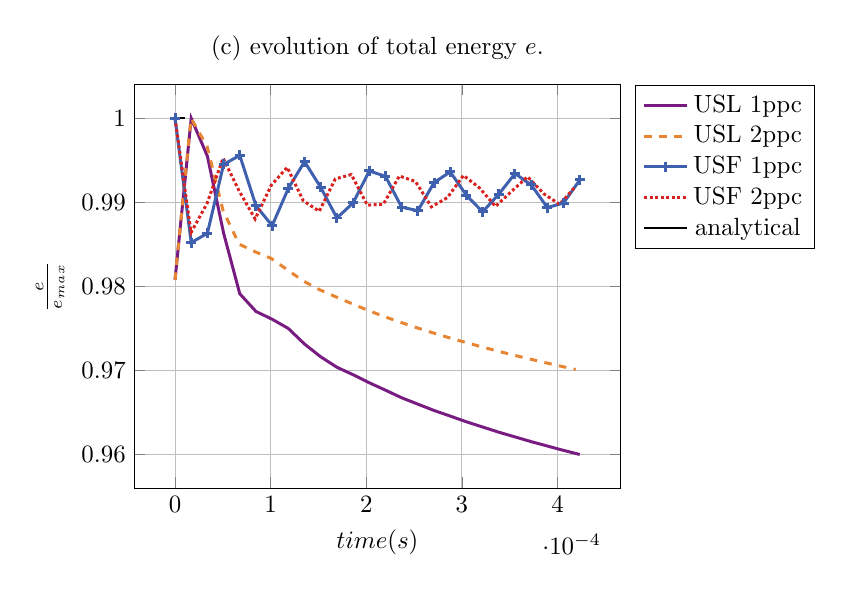
\begin{tikzpicture}[scale=0.9]
\begin{axis}[xlabel=$time (s)$,ylabel=$\frac{e}{e_{max}}$,ymajorgrids=true,xmajorgrids=true,title={(c) evolution of total energy $e$.},legend pos=outer north east]
\addplot[Purple,very thick,mark=none,solid] coordinates {(0.0,0.980776775206) (1.69272151355e-05,1.0) (3.38544302711e-05,0.995486386818) (5.07816454066e-05,0.986335480918) (6.77088605422e-05,0.979118179787) (8.46360756777e-05,0.977011836735) (0.000101563290813,0.976083552705) (0.000118490505949,0.974985958077) (0.000135417721084,0.973132007483) (0.00015234493622,0.971614043952) (0.000169272151355,0.970370597838) (0.000186199366491,0.969484052645) (0.000203126581626,0.968527091175) (0.000220053796762,0.967645365047) (0.000236981011898,0.966743210911) (0.000253908227033,0.965982183586) (0.000270835442169,0.965231974397) (0.000287762657304,0.964563191524) (0.00030468987244,0.96388114719) (0.000321617087575,0.963263530823) (0.000338544302711,0.962646353557) (0.000355471517846,0.962084695394) (0.000372398732982,0.961521764293) (0.000389325948117,0.961001071279) (0.000406253163253,0.960479919884) (0.000423180378389,0.959994795728) };
\addplot[Orange,very thick,mark=none,dashed] coordinates {(0.0,0.980776775206) (1.67562331645e-05,1.0) (3.3512466329e-05,0.996663809337) (5.02686994934e-05,0.98900666995) (6.70249326579e-05,0.985020324447) (8.37811658224e-05,0.984110580813) (0.000100537398987,0.983326915208) (0.000117293632151,0.981979184866) (0.000134049865316,0.980638155666) (0.00015080609848,0.979617302856) (0.000167562331645,0.978778886884) (0.000184318564809,0.977968446843) (0.000201074797974,0.977176694993) (0.000217831031138,0.976440965591) (0.000234587264303,0.975764557777) (0.000251343497467,0.975128766754) (0.000268099730632,0.974522184343) (0.000284855963796,0.973943735564) (0.000301612196961,0.973393220953) (0.000318368430125,0.972867749193) (0.00033512466329,0.972363947434) (0.000351880896454,0.971879647077) (0.000368637129618,0.971413467384) (0.000385393362783,0.970964070517) (0.000402149595947,0.97053007437) (0.000418905829112,0.970110254428) };
\addplot[Blue,very thick,mark=+,solid] coordinates {(0.0,1.0) (1.69272151355e-05,0.985202) (3.38544302711e-05,0.986310925125) (5.07816454066e-05,0.994507638064) (6.77088605422e-05,0.995579868604) (8.46360756777e-05,0.989584575004) (0.000101563290813,0.987225270569) (0.000118490505949,0.991657283729) (0.000135417721084,0.994836102021) (0.00015234493622,0.991773304725) (0.000169272151355,0.988131314159) (0.000186199366491,0.989928559949) (0.000203126581626,0.993725892454) (0.000220053796762,0.993092827557) (0.000236981011898,0.989412077079) (0.000253908227033,0.989007930164) (0.000270835442169,0.992337891088) (0.000287762657304,0.993619763816) (0.00030468987244,0.990831091012) (0.000321617087575,0.988860712515) (0.000338544302711,0.990967493415) (0.000355471517846,0.993415506334) (0.000372398732982,0.99207684926) (0.000389325948117,0.989372657972) (0.000406253163253,0.98991313843) (0.000423180378389,0.992654041387) };
\addplot[Red,very thick,mark=none,densely dotted] coordinates {(0.0,1.0) (1.67562331645e-05,0.9864025) (3.3512466329e-05,0.989873766211) (5.02686994934e-05,0.995255572924) (6.70249326579e-05,0.991355462516) (8.37811658224e-05,0.988011538229) (0.000100537398987,0.992011167376) (0.000117293632151,0.994160481387) (0.000134049865316,0.990189454195) (0.00015080609848,0.988933325063) (0.000167562331645,0.992779930372) (0.000184318564809,0.993300645038) (0.000201074797974,0.989660626012) (0.000217831031138,0.98976821642) (0.000234587264303,0.993129965182) (0.000251343497467,0.992481697852) (0.000268099730632,0.989459518699) (0.000284855963796,0.990567889043) (0.000301612196961,0.993200218105) (0.000318368430125,0.991710475421) (0.00033512466329,0.989506548964) (0.000351880896454,0.99129883371) (0.000368637129618,0.993048080156) (0.000385393362783,0.99103246412) (0.000402149595947,0.989751621209) (0.000418905829112,0.99191164529) };
\addplot[black,thick] coordinates {(0.,1.) (0.00001,1.)};
\legend{USL 1ppc,USL 2ppc,USF 1ppc,USF 2ppc,analytical}
\end{axis}
\end{tikzpicture}
 \phantomsubcaption \label{subfig:US_energies}}
  \caption{MPM solutions of the bars impact problem for various discretizations. (a)--(b) comparison of stress computed with USF and USL formulations and exact solutions (c) numerical total energy evolutions. Parameters: $CFL=0.7$ ; $v_0=\frac{1}{200}\sqrt{\frac{E}{\rho}}$.}
  \label{fig:US_diffusion}
\end{figure}
Figures \ref{fig:US_diffusion}\subref{subfig:US_diffusion_10} and \ref{fig:US_diffusion}\subref{subfig:US_diffusion_25} show that both USL and USF solutions oscillate after the passage of the elastic front. Those oscillations are much more significant in the USF solutions regardless of the number of particles used. Indeed, the noise in USL results quickly reduces so that the correct stress level is reached in the middle region of the bar. Moreover, even though the $1\: ppc$ and $2\: ppc$ discretizations provide different results (slightly different for USL), neither of them enables the removal of oscillations. Figure \ref{fig:US_diffusion}\subref{subfig:US_energies} shows, on the other hand, the evolutions of numerical total energies. Note that the total energy results from an MPM approximation of kinetic and strain energies, respectively defined as:
\begin{align}
  & e^{kin}=\frac{1}{2}\int_\Omega \rho \vect{v}\cdot\vect{v} \:d\Omega \approx \frac{1}{2}\sum_p m_p \vect{v}^p\cdot\vect{v}^p\\
& e^{strain}= \frac{1}{2}\int_\Omega \rho \tens{\bar{\sigma}}: \nablav \vect{v} \:d\Omega \approx \frac{1}{2}\sum_p m_p \tens{\bar{\sigma}}^p: \nablav \vect{v}^p
\end{align}
One can see that the USL formulation is more diffusive than the USF for this problem. These results differ from observations made in \cite{Bardenhagen_USF_USL}, in which no significant difference appears in energy plots for problems involving smooth solutions. At last, figure \ref{fig:US_velocities} compares the numerical velocities to the exact solution at various time steps. The same pattern than that observed for stresses is seen in figures \ref{fig:US_velocities}\subref{subfig:US_velo_10} and \ref{fig:US_velocities}\subref{subfig:US_velo_25} for velocities, namely, numerical oscillations in both USL and USF solutions with bigger picks in the USF ones. 

A notable numerical artifact that prevents the proper assessment of the velocity occurs at the middle of the bar. This issue is not due to the computation of internal forces since the symmetrical stress solutions plotted in figures \ref{fig:US_diffusion}\subref{subfig:US_diffusion_10} and \ref{fig:US_diffusion}\subref{subfig:US_diffusion_25}, combined to the discontinuous gradient of shape functions, yield zero internal forces at the central node of the computational grid (equation \eqref{eq:int_forces}). Furthermore, a skew-symmetric velocity solution leads, after the convective step, to a zero velocity at the central node, which is the correct solution (and never changes because of null internal forces). Hence, the error most likely comes from the back-mapping of fields from the grid to material points. 
\begin{figure}[h!]
  \centering
  {\definecolor{Purple}{RGB}{120,28,129}
\definecolor{Orange}{RGB}{231,133,50}
\definecolor{Blue}{RGB}{63,96,174}
\definecolor{Red}{RGB}{217,33,32}
\definecolor{Duck}{RGB}{83,158,182}
\definecolor{Green}{RGB}{109,179,136}
\definecolor{Yellow}{RGB}{202,184,67}
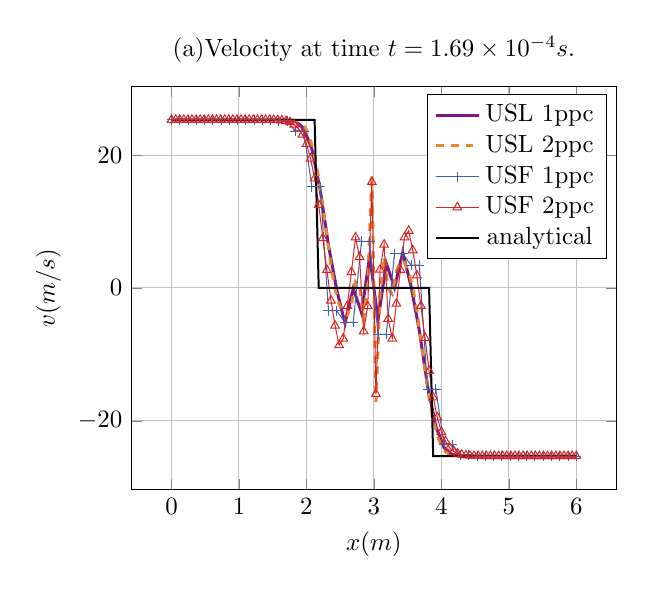
\begin{tikzpicture}[scale=0.9]
\begin{axis}[xlabel=$x (m)$,ylabel=$v (m/s)$,ymajorgrids=true,xmajorgrids=true,title={(a)Velocity at time $t=1.69\times 10^{-4}s.$}]
\addplot[Purple,very thick,mark=none,solid] coordinates {(0.0,25.3184841771) (0.122448979592,25.3184841771) (0.244897959184,25.3184841771) (0.367346938776,25.3184841771) (0.489795918367,25.3184841771) (0.612244897959,25.3184841771) (0.734693877551,25.3184841771) (0.857142857143,25.3184841771) (0.979591836735,25.3184841771) (1.10204081633,25.3184841771) (1.22448979592,25.3184841771) (1.34693877551,25.3184841771) (1.4693877551,25.3184841771) (1.59183673469,25.3184841771) (1.71428571429,25.3184841771) (1.83673469388,25.1149797615) (1.95918367347,24.0545424864) (2.08163265306,20.8743509476) (2.20408163265,14.7547033581) (2.32653061224,6.41598558277) (2.44897959184,-0.244456370035) (2.57142857143,-5.35821612759) (2.69387755102,-0.0619763112976) (2.81632653061,-3.709401685) (2.9387755102,4.8348853161) (3.0612244898,-4.8348853161) (3.18367346939,3.709401685) (3.30612244898,0.0619763112976) (3.42857142857,5.35821612759) (3.55102040816,0.244456370035) (3.67346938776,-6.41598558277) (3.79591836735,-14.7547033581) (3.91836734694,-20.8743509476) (4.04081632653,-24.0545424864) (4.16326530612,-25.1149797615) (4.28571428571,-25.3184841771) (4.40816326531,-25.3184841771) (4.5306122449,-25.3184841771) (4.65306122449,-25.3184841771) (4.77551020408,-25.3184841771) (4.89795918367,-25.3184841771) (5.02040816327,-25.3184841771) (5.14285714286,-25.3184841771) (5.26530612245,-25.3184841771) (5.38775510204,-25.3184841771) (5.51020408163,-25.3184841771) (5.63265306122,-25.3184841771) (5.75510204082,-25.3184841771) (5.87755102041,-25.3184841771) (6.0,-25.3184841771) };
\addplot[Orange,very thick,mark=none,dashed] coordinates {(0.0,25.3184841771) (0.0606060606061,25.3184841771) (0.121212121212,25.3184841771) (0.181818181818,25.3184841771) (0.242424242424,25.3184841771) (0.30303030303,25.3184841771) (0.363636363636,25.3184841771) (0.424242424242,25.3184841771) (0.484848484848,25.3184841771) (0.545454545455,25.3184841771) (0.606060606061,25.3184841771) (0.666666666667,25.3184841771) (0.727272727273,25.3184841771) (0.787878787879,25.3184841771) (0.848484848485,25.3184841771) (0.909090909091,25.3184841771) (0.969696969697,25.3184841771) (1.0303030303,25.3184841771) (1.09090909091,25.3184841771) (1.15151515152,25.3184841771) (1.21212121212,25.3184841771) (1.27272727273,25.3184841771) (1.33333333333,25.3184841771) (1.39393939394,25.3184841771) (1.45454545455,25.3184841771) (1.51515151515,25.3184841771) (1.57575757576,25.3184841771) (1.63636363636,25.3184841771) (1.69696969697,25.3184841771) (1.75757575758,25.3184841771) (1.81818181818,25.251933876) (1.87878787879,25.1188332739) (1.93939393939,24.6493504882) (2.0,23.8434855187) (2.06060606061,22.247450502) (2.12121212121,19.8612454379) (2.18181818182,16.5614104839) (2.24242424242,12.3479456399) (2.30303030303,7.94379399222) (2.36363636364,3.34895554082) (2.42424242424,-0.133198996542) (2.48484848485,-2.50266961986) (2.54545454545,-3.82041358095) (2.60606060606,-4.08643087983) (2.66666666667,-2.50894819569) (2.72727272727,0.91203447147) (2.78787878788,0.178185932665) (2.84848484848,-4.71049381211) (2.90909090909,0.963495780905) (2.9696969697,17.2001547117) (3.0303030303,-17.2001547117) (3.09090909091,-0.963495780905) (3.15151515152,4.7104938121) (3.21212121212,-0.178185932665) (3.27272727273,-0.91203447147) (3.33333333333,2.50894819569) (3.39393939394,4.08643087983) (3.45454545455,3.82041358095) (3.51515151515,2.50266961986) (3.57575757576,0.133198996542) (3.63636363636,-3.34895554082) (3.69696969697,-7.94379399222) (3.75757575758,-12.3479456399) (3.81818181818,-16.5614104839) (3.87878787879,-19.8612454379) (3.93939393939,-22.247450502) (4.0,-23.8434855187) (4.06060606061,-24.6493504882) (4.12121212121,-25.1188332739) (4.18181818182,-25.251933876) (4.24242424242,-25.3184841771) (4.30303030303,-25.3184841771) (4.36363636364,-25.3184841771) (4.42424242424,-25.3184841771) (4.48484848485,-25.3184841771) (4.54545454545,-25.3184841771) (4.60606060606,-25.3184841771) (4.66666666667,-25.3184841771) (4.72727272727,-25.3184841771) (4.78787878788,-25.3184841771) (4.84848484848,-25.3184841771) (4.90909090909,-25.3184841771) (4.9696969697,-25.3184841771) (5.0303030303,-25.3184841771) (5.09090909091,-25.3184841771) (5.15151515152,-25.3184841771) (5.21212121212,-25.3184841771) (5.27272727273,-25.3184841771) (5.33333333333,-25.3184841771) (5.39393939394,-25.3184841771) (5.45454545455,-25.3184841771) (5.51515151515,-25.3184841771) (5.57575757576,-25.3184841771) (5.63636363636,-25.3184841771) (5.69696969697,-25.3184841771) (5.75757575758,-25.3184841771) (5.81818181818,-25.3184841771) (5.87878787879,-25.3184841771) (5.93939393939,-25.3184841771) (6.0,-25.3184841771) };
\addplot[Blue,thin,mark=+,solid] coordinates {(0.0,25.3184841771) (0.122448979592,25.3184841771) (0.244897959184,25.3184841771) (0.367346938776,25.3184841771) (0.489795918367,25.3184841771) (0.612244897959,25.3184841386) (0.734693877551,25.3184841386) (0.857142857143,25.3184789327) (0.979591836735,25.3184789327) (1.10204081633,25.3181863193) (1.22448979592,25.3181863193) (1.34693877551,25.3093479957) (1.4693877551,25.3093479957) (1.59183673469,25.1550198372) (1.71428571429,25.1550198372) (1.83673469388,23.6026380028) (1.95918367347,23.6026380028) (2.08163265306,15.2761405323) (2.20408163265,15.2761405323) (2.32653061224,-3.42382560915) (2.44897959184,-3.42382560915) (2.57142857143,-5.17320665774) (2.69387755102,-5.17320665774) (2.81632653061,6.99898825925) (2.9387755102,6.99898825925) (3.0612244898,-6.99898825925) (3.18367346939,-6.99898825925) (3.30612244898,5.17320665774) (3.42857142857,5.17320665774) (3.55102040816,3.42382560915) (3.67346938776,3.42382560915) (3.79591836735,-15.2761405323) (3.91836734694,-15.2761405323) (4.04081632653,-23.6026380028) (4.16326530612,-23.6026380028) (4.28571428571,-25.1550198372) (4.40816326531,-25.1550198372) (4.5306122449,-25.3093479957) (4.65306122449,-25.3093479957) (4.77551020408,-25.3181863193) (4.89795918367,-25.3181863193) (5.02040816327,-25.3184789327) (5.14285714286,-25.3184789327) (5.26530612245,-25.3184841386) (5.38775510204,-25.3184841386) (5.51020408163,-25.3184841771) (5.63265306122,-25.3184841771) (5.75510204082,-25.3184841771) (5.87755102041,-25.3184841771) (6.0,-25.3184841771) };
\addplot[Red,thin,mark=triangle,solid] coordinates {(0.0,25.3184841771) (0.0606060606061,25.3184841771) (0.121212121212,25.3184841771) (0.181818181818,25.3184841771) (0.242424242424,25.3184841771) (0.30303030303,25.3184841771) (0.363636363636,25.3184841771) (0.424242424242,25.3184841771) (0.484848484848,25.3184841771) (0.545454545455,25.3184841771) (0.606060606061,25.3184841756) (0.666666666667,25.3184841728) (0.727272727273,25.3184841554) (0.787878787879,25.3184841236) (0.848484848485,25.3184837955) (0.909090909091,25.3184831711) (0.969696969697,25.3184803575) (1.0303030303,25.3184753545) (1.09090909091,25.3184471873) (1.15151515152,25.3183958557) (1.21212121212,25.3182145032) (1.27272727273,25.3179031296) (1.33333333333,25.3166920979) (1.39393939394,25.3145814079) (1.45454545455,25.3086270817) (1.51515151515,25.2988291195) (1.57575757576,25.2705514254) (1.63636363636,25.2237939997) (1.69696969697,25.1183204342) (1.75757575758,24.9541307292) (1.81818181818,24.5979538878) (1.87878787879,24.0497899101) (1.93939393939,23.076688448) (2.0,21.6786495014) (2.06060606061,19.4833431738) (2.12121212121,16.4907694654) (2.18181818182,12.4989085572) (2.24242424242,7.50776044936) (2.30303030303,2.70872378788) (2.36363636364,-1.89820142723) (2.42424242424,-5.67144294529) (2.48484848485,-8.61100076632) (2.54545454545,-7.62326403856) (2.60606060606,-2.70823276202) (2.66666666667,2.3712989244) (2.72727272727,7.61533102071) (2.78787878788,4.6503105848) (2.84848484848,-6.52376238331) (2.90909090909,-2.75347810625) (2.9696969697,15.961163416) (3.0303030303,-15.961163416) (3.09090909091,2.75347810625) (3.15151515152,6.52376238331) (3.21212121212,-4.6503105848) (3.27272727273,-7.61533102071) (3.33333333333,-2.3712989244) (3.39393939394,2.70823276202) (3.45454545455,7.62326403856) (3.51515151515,8.61100076632) (3.57575757576,5.67144294529) (3.63636363636,1.89820142723) (3.69696969697,-2.70872378788) (3.75757575758,-7.50776044936) (3.81818181818,-12.4989085572) (3.87878787879,-16.4907694654) (3.93939393939,-19.4833431738) (4.0,-21.6786495014) (4.06060606061,-23.076688448) (4.12121212121,-24.0497899101) (4.18181818182,-24.5979538878) (4.24242424242,-24.9541307292) (4.30303030303,-25.1183204342) (4.36363636364,-25.2237939997) (4.42424242424,-25.2705514254) (4.48484848485,-25.2988291195) (4.54545454545,-25.3086270817) (4.60606060606,-25.3145814079) (4.66666666667,-25.3166920979) (4.72727272727,-25.3179031296) (4.78787878788,-25.3182145032) (4.84848484848,-25.3183958557) (4.90909090909,-25.3184471873) (4.9696969697,-25.3184753545) (5.0303030303,-25.3184803575) (5.09090909091,-25.3184831711) (5.15151515152,-25.3184837955) (5.21212121212,-25.3184841236) (5.27272727273,-25.3184841554) (5.33333333333,-25.3184841728) (5.39393939394,-25.3184841756) (5.45454545455,-25.3184841771) (5.51515151515,-25.3184841771) (5.57575757576,-25.3184841771) (5.63636363636,-25.3184841771) (5.69696969697,-25.3184841771) (5.75757575758,-25.3184841771) (5.81818181818,-25.3184841771) (5.87878787879,-25.3184841771) (5.93939393939,-25.3184841771) (6.0,-25.3184841771) };
\addplot[black,thick,mark=none,solid] coordinates {(0.0,25.3184841771) (0.0606060606061,25.3184841771) (0.121212121212,25.3184841771) (0.181818181818,25.3184841771) (0.242424242424,25.3184841771) (0.30303030303,25.3184841771) (0.363636363636,25.3184841771) (0.424242424242,25.3184841771) (0.484848484848,25.3184841771) (0.545454545455,25.3184841771) (0.606060606061,25.3184841771) (0.666666666667,25.3184841771) (0.727272727273,25.3184841771) (0.787878787879,25.3184841771) (0.848484848485,25.3184841771) (0.909090909091,25.3184841771) (0.969696969697,25.3184841771) (1.0303030303,25.3184841771) (1.09090909091,25.3184841771) (1.15151515152,25.3184841771) (1.21212121212,25.3184841771) (1.27272727273,25.3184841771) (1.33333333333,25.3184841771) (1.39393939394,25.3184841771) (1.45454545455,25.3184841771) (1.51515151515,25.3184841771) (1.57575757576,25.3184841771) (1.63636363636,25.3184841771) (1.69696969697,25.3184841771) (1.75757575758,25.3184841771) (1.81818181818,25.3184841771) (1.87878787879,25.3184841771) (1.93939393939,25.3184841771) (2.0,25.3184841771) (2.06060606061,25.3184841771) (2.12121212121,25.3184841771) (2.18181818182,0.0) (2.24242424242,0.0) (2.30303030303,0.0) (2.36363636364,0.0) (2.42424242424,0.0) (2.48484848485,0.0) (2.54545454545,0.0) (2.60606060606,0.0) (2.66666666667,0.0) (2.72727272727,0.0) (2.78787878788,0.0) (2.84848484848,0.0) (2.90909090909,0.0) (2.9696969697,0.0) (3.0303030303,-0.0) (3.09090909091,-0.0) (3.15151515152,-0.0) (3.21212121212,-0.0) (3.27272727273,-0.0) (3.33333333333,-0.0) (3.39393939394,-0.0) (3.45454545455,-0.0) (3.51515151515,-0.0) (3.57575757576,-0.0) (3.63636363636,-0.0) (3.69696969697,-0.0) (3.75757575758,-0.0) (3.81818181818,-0.0) (3.87878787879,-25.3184841771) (3.93939393939,-25.3184841771) (4.0,-25.3184841771) (4.06060606061,-25.3184841771) (4.12121212121,-25.3184841771) (4.18181818182,-25.3184841771) (4.24242424242,-25.3184841771) (4.30303030303,-25.3184841771) (4.36363636364,-25.3184841771) (4.42424242424,-25.3184841771) (4.48484848485,-25.3184841771) (4.54545454545,-25.3184841771) (4.60606060606,-25.3184841771) (4.66666666667,-25.3184841771) (4.72727272727,-25.3184841771) (4.78787878788,-25.3184841771) (4.84848484848,-25.3184841771) (4.90909090909,-25.3184841771) (4.9696969697,-25.3184841771) (5.0303030303,-25.3184841771) (5.09090909091,-25.3184841771) (5.15151515152,-25.3184841771) (5.21212121212,-25.3184841771) (5.27272727273,-25.3184841771) (5.33333333333,-25.3184841771) (5.39393939394,-25.3184841771) (5.45454545455,-25.3184841771) (5.51515151515,-25.3184841771) (5.57575757576,-25.3184841771) (5.63636363636,-25.3184841771) (5.69696969697,-25.3184841771) (5.75757575758,-25.3184841771) (5.81818181818,-25.3184841771) (5.87878787879,-25.3184841771) (5.93939393939,-25.3184841771) (6.0,-25.3184841771) };
\legend{USL 1ppc,USL 2ppc,USF 1ppc,USF 2ppc,analytical}
\end{axis}
\end{tikzpicture}

%%% Local Variables: 
%%% mode: latex
%%% TeX-master: "../../mainManuscript"
%%% End:
\phantomsubcaption \label{subfig:US_velo_10}}
  {\definecolor{Purple}{RGB}{120,28,129}
\definecolor{Orange}{RGB}{231,133,50}
\definecolor{Blue}{RGB}{63,96,174}
\definecolor{Red}{RGB}{217,33,32}
\definecolor{Duck}{RGB}{83,158,182}
\definecolor{Green}{RGB}{109,179,136}
\definecolor{Yellow}{RGB}{202,184,67}
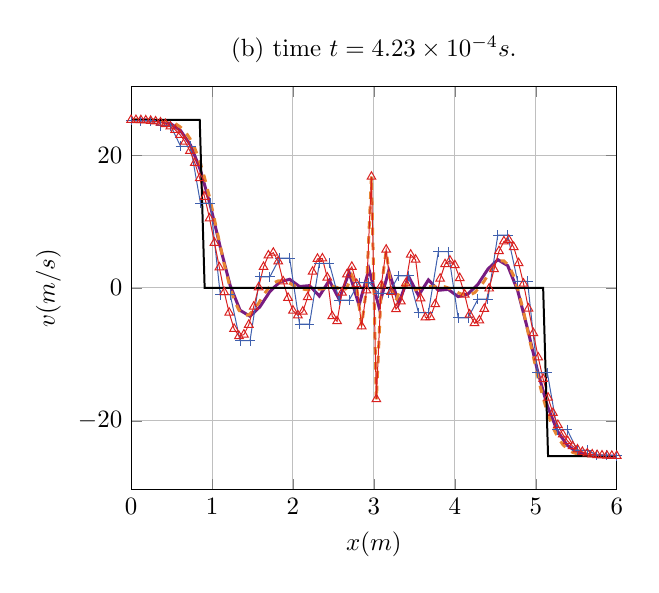
\begin{tikzpicture}[scale=0.9]
\begin{axis}[xlabel=$x (m)$,ylabel=$v (m/s)$,ymajorgrids=true,xmajorgrids=true,title={(b) time $t=4.23 \times 10^{-4}s$.},xmin=0.,xmax=6.]
\addplot[Purple,very thick,mark=none,solid] coordinates {(0.0,25.3179577559) (0.122448979592,25.3125244526) (0.244897959184,25.2804932478) (0.367346938776,25.1489907367) (0.489795918367,24.7341796044) (0.612244897959,23.6864809647) (0.734693877551,21.5118739395) (0.857142857143,17.7671095652) (0.979591836735,12.4121755247) (1.10204081633,6.14683940753) (1.22448979592,0.373716046882) (1.34693877551,-3.3616057723) (1.4693877551,-4.26176674269) (1.59183673469,-2.83406587609) (1.71428571429,-0.55562049587) (1.83673469388,0.901404345798) (1.95918367347,1.30403292578) (2.08163265306,0.214501074535) (2.20408163265,0.352209313776) (2.32653061224,-1.21718822558) (2.44897959184,1.14054029809) (2.57142857143,-1.72149525556) (2.69387755102,2.335373076) (2.81632653061,-2.59610029814) (2.9387755102,2.82071480229) (3.0612244898,-2.82071480229) (3.18367346939,2.59610029814) (3.30612244898,-2.335373076) (3.42857142857,1.72149525556) (3.55102040816,-1.14054029809) (3.67346938776,1.21718822558) (3.79591836735,-0.352209313776) (3.91836734694,-0.214501074535) (4.04081632653,-1.30403292578) (4.16326530612,-0.901404345798) (4.28571428571,0.55562049587) (4.40816326531,2.83406587609) (4.5306122449,4.26176674269) (4.65306122449,3.3616057723) (4.77551020408,-0.373716046882) (4.89795918367,-6.14683940753) (5.02040816327,-12.4121755247) (5.14285714286,-17.7671095652) (5.26530612245,-21.5118739395) (5.38775510204,-23.6864809647) (5.51020408163,-24.7341796044) (5.63265306122,-25.1489907367) (5.75510204082,-25.2804932478) (5.87755102041,-25.3125244526) (6.0,-25.3179577559) };
\addplot[Orange,very thick,mark=none,dashed] coordinates {(0.0,25.3184113784) (0.0606060606061,25.3182657812) (0.121212121212,25.3171343813) (0.181818181818,25.3150171787) (0.242424242424,25.3062460446) (0.30303030303,25.2908209787) (0.363636363636,25.2461773758) (0.424242424242,25.1723152357) (0.484848484848,25.0062868064) (0.545454545455,24.748092088) (0.606060606061,24.2720385643) (0.666666666667,23.5781262352) (0.727272727273,22.4951335769) (0.787878787879,21.0230605893) (0.848484848485,19.0428242456) (0.909090909091,16.5544245458) (0.969696969697,13.6460768618) (1.0303030303,10.3177811934) (1.09090909091,6.94923058708) (1.15151515152,3.54042504293) (1.21212121212,0.626561316633) (1.27272727273,-1.79236059183) (1.33333333333,-3.36301978655) (1.39393939394,-4.08541626753) (1.45454545455,-4.06554257142) (1.51515151515,-3.30339869822) (1.57575757576,-2.29577774705) (1.63636363636,-1.04267971791) (1.69696969697,-0.0393881478233) (1.75757575758,0.714096963215) (1.81818181818,1.07591385411) (1.87878787879,1.04606252486) (1.93939393939,0.832069940855) (2.0,0.433936102092) (2.06060606061,0.100491892604) (2.12121212121,-0.168262687611) (2.18181818182,-0.281962807299) (2.24242424242,-0.24060846646) (2.30303030303,-0.19473430746) (2.36363636364,-0.144340330301) (2.42424242424,0.0103021847971) (2.48484848485,0.269193237834) (2.54545454545,0.0743373654573) (2.60606060606,-0.574265432333) (2.66666666667,0.0252212025898) (2.72727272727,1.87279727022) (2.78787878788,-0.017779131944) (2.84848484848,-5.64650800392) (2.90909090909,-0.0160332856532) (2.9696969697,16.8736450228) (3.0303030303,-16.8736450228) (3.09090909091,0.0160332856532) (3.15151515152,5.64650800392) (3.21212121212,0.017779131944) (3.27272727273,-1.87279727022) (3.33333333333,-0.0252212025898) (3.39393939394,0.574265432333) (3.45454545455,-0.0743373654573) (3.51515151515,-0.269193237834) (3.57575757576,-0.0103021847971) (3.63636363636,0.144340330301) (3.69696969697,0.19473430746) (3.75757575758,0.24060846646) (3.81818181818,0.281962807299) (3.87878787879,0.168262687611) (3.93939393939,-0.100491892604) (4.0,-0.433936102092) (4.06060606061,-0.832069940855) (4.12121212121,-1.04606252486) (4.18181818182,-1.07591385411) (4.24242424242,-0.714096963215) (4.30303030303,0.0393881478233) (4.36363636364,1.04267971791) (4.42424242424,2.29577774705) (4.48484848485,3.30339869822) (4.54545454545,4.06554257142) (4.60606060606,4.08541626753) (4.66666666667,3.36301978655) (4.72727272727,1.79236059183) (4.78787878788,-0.626561316633) (4.84848484848,-3.54042504293) (4.90909090909,-6.94923058708) (4.9696969697,-10.3177811934) (5.0303030303,-13.6460768618) (5.09090909091,-16.5544245458) (5.15151515152,-19.0428242456) (5.21212121212,-21.0230605893) (5.27272727273,-22.4951335769) (5.33333333333,-23.5781262352) (5.39393939394,-24.2720385643) (5.45454545455,-24.748092088) (5.51515151515,-25.0062868064) (5.57575757576,-25.1723152357) (5.63636363636,-25.2461773758) (5.69696969697,-25.2908209787) (5.75757575758,-25.3062460446) (5.81818181818,-25.3150171787) (5.87878787879,-25.3171343813) (5.93939393939,-25.3182657812) (6.0,-25.3184113784) };
\addplot[Blue,thin,mark=+,solid] coordinates {(0.0,25.278692227) (0.122448979592,25.1632638972) (0.244897959184,25.1632638972) (0.367346938776,24.4134945697) (0.489795918367,24.4134945697) (0.612244897959,21.3339382893) (0.734693877551,21.3339382893) (0.857142857143,12.7864947989) (0.979591836735,12.7864947989) (1.10204081633,-1.00143026403) (1.22448979592,-1.00143026403) (1.34693877551,-7.94234859658) (1.4693877551,-7.94234859658) (1.59183673469,1.666718506) (1.71428571429,1.666718506) (1.83673469388,4.4983018773) (1.95918367347,4.4983018773) (2.08163265306,-5.4528024961) (2.20408163265,-5.4528024961) (2.32653061224,3.70951010765) (2.44897959184,3.70951010765) (2.57142857143,-1.8372342386) (2.69387755102,-1.8372342386) (2.81632653061,0.817767529336) (2.9387755102,0.817767529337) (3.0612244898,-0.817767529337) (3.18367346939,-0.817767529336) (3.30612244898,1.8372342386) (3.42857142857,1.8372342386) (3.55102040816,-3.70951010765) (3.67346938776,-3.70951010765) (3.79591836735,5.4528024961) (3.91836734694,5.4528024961) (4.04081632653,-4.4983018773) (4.16326530612,-4.4983018773) (4.28571428571,-1.666718506) (4.40816326531,-1.666718506) (4.5306122449,7.94234859658) (4.65306122449,7.94234859658) (4.77551020408,1.00143026403) (4.89795918367,1.00143026403) (5.02040816327,-12.7864947989) (5.14285714286,-12.7864947989) (5.26530612245,-21.3339382893) (5.38775510204,-21.3339382893) (5.51020408163,-24.4134945697) (5.63265306122,-24.4134945697) (5.75510204082,-25.1632638972) (5.87755102041,-25.1632638972) (6.0,-25.278692227) };
\addplot[Red,thin,mark=triangle,solid] coordinates {(0.0,25.2925663718) (0.0606060606061,25.2843839677) (0.121212121212,25.2634771526) (0.181818181818,25.2298459266) (0.242424242424,25.166861976) (0.30303030303,25.074525301) (0.363636363636,24.9151607465) (0.424242424242,24.6887683126) (0.484848484848,24.3234854983) (0.545454545455,23.8193123035) (0.606060606061,23.0610017936) (0.666666666667,22.0485539687) (0.727272727273,20.638560445) (0.787878787879,18.8310212227) (0.848484848485,16.5222107775) (0.909090909091,13.7121291096) (0.969696969697,10.4726131337) (1.0303030303,6.80366284984) (1.09090909091,3.09745596005) (1.15151515152,-0.646007535703) (1.21212121212,-3.7294710718) (1.27272727273,-6.15293464823) (1.33333333333,-7.25044901317) (1.39393939394,-7.02201416662) (1.45454545455,-5.54409239748) (1.51515151515,-2.81668370575) (1.57575757576,0.0833596298948) (1.63636363636,3.15603760945) (1.69696969697,4.89643176607) (1.75757575758,5.30454209975) (1.81818181818,4.00211543869) (1.87878787879,0.98915178291) (1.93939393939,-1.48619261955) (2.0,-3.42391776869) (2.06060606061,-4.1204907004) (2.12121212121,-3.57591141468) (2.18181818182,-1.3875328666) (2.24242424242,2.44464494385) (2.30303030303,4.38796385565) (2.36363636364,4.44242386881) (2.42424242424,1.55990936166) (2.48484848485,-4.2595796658) (2.54545454545,-5.01317341167) (2.60606060606,-0.700871875953) (2.66666666667,2.03314306079) (2.72727272727,3.18887139857) (2.78787878788,0.588067826574) (2.84848484848,-5.76926765519) (2.90909090909,-0.381330502781) (2.9696969697,16.7518792838) (3.0303030303,-16.7518792838) (3.09090909091,0.381330502781) (3.15151515152,5.76926765519) (3.21212121212,-0.588067826574) (3.27272727273,-3.18887139857) (3.33333333333,-2.03314306079) (3.39393939394,0.700871875953) (3.45454545455,5.01317341167) (3.51515151515,4.2595796658) (3.57575757576,-1.55990936166) (3.63636363636,-4.44242386881) (3.69696969697,-4.38796385565) (3.75757575758,-2.44464494385) (3.81818181818,1.3875328666) (3.87878787879,3.57591141468) (3.93939393939,4.1204907004) (4.0,3.42391776869) (4.06060606061,1.48619261955) (4.12121212121,-0.98915178291) (4.18181818182,-4.00211543869) (4.24242424242,-5.30454209975) (4.30303030303,-4.89643176607) (4.36363636364,-3.15603760945) (4.42424242424,-0.0833596298948) (4.48484848485,2.81668370575) (4.54545454545,5.54409239748) (4.60606060606,7.02201416662) (4.66666666667,7.25044901317) (4.72727272727,6.15293464823) (4.78787878788,3.7294710718) (4.84848484848,0.646007535703) (4.90909090909,-3.09745596005) (4.9696969697,-6.80366284984) (5.0303030303,-10.4726131337) (5.09090909091,-13.7121291096) (5.15151515152,-16.5222107775) (5.21212121212,-18.8310212227) (5.27272727273,-20.638560445) (5.33333333333,-22.0485539687) (5.39393939394,-23.0610017936) (5.45454545455,-23.8193123035) (5.51515151515,-24.3234854983) (5.57575757576,-24.6887683126) (5.63636363636,-24.9151607465) (5.69696969697,-25.074525301) (5.75757575758,-25.166861976) (5.81818181818,-25.2298459266) (5.87878787879,-25.2634771526) (5.93939393939,-25.2843839677) (6.0,-25.2925663718) };
\addplot[black,thick,mark=none,solid] coordinates {(0.0,25.3184841771) (0.0606060606061,25.3184841771) (0.121212121212,25.3184841771) (0.181818181818,25.3184841771) (0.242424242424,25.3184841771) (0.30303030303,25.3184841771) (0.363636363636,25.3184841771) (0.424242424242,25.3184841771) (0.484848484848,25.3184841771) (0.545454545455,25.3184841771) (0.606060606061,25.3184841771) (0.666666666667,25.3184841771) (0.727272727273,25.3184841771) (0.787878787879,25.3184841771) (0.848484848485,25.3184841771) (0.909090909091,0.0) (0.969696969697,0.0) (1.0303030303,0.0) (1.09090909091,0.0) (1.15151515152,0.0) (1.21212121212,0.0) (1.27272727273,0.0) (1.33333333333,0.0) (1.39393939394,0.0) (1.45454545455,0.0) (1.51515151515,0.0) (1.57575757576,0.0) (1.63636363636,0.0) (1.69696969697,0.0) (1.75757575758,0.0) (1.81818181818,0.0) (1.87878787879,0.0) (1.93939393939,0.0) (2.0,0.0) (2.06060606061,0.0) (2.12121212121,0.0) (2.18181818182,0.0) (2.24242424242,0.0) (2.30303030303,0.0) (2.36363636364,0.0) (2.42424242424,0.0) (2.48484848485,0.0) (2.54545454545,0.0) (2.60606060606,0.0) (2.66666666667,0.0) (2.72727272727,0.0) (2.78787878788,0.0) (2.84848484848,0.0) (2.90909090909,0.0) (2.9696969697,0.0) (3.0303030303,-0.0) (3.09090909091,-0.0) (3.15151515152,-0.0) (3.21212121212,-0.0) (3.27272727273,-0.0) (3.33333333333,-0.0) (3.39393939394,-0.0) (3.45454545455,-0.0) (3.51515151515,-0.0) (3.57575757576,-0.0) (3.63636363636,-0.0) (3.69696969697,-0.0) (3.75757575758,-0.0) (3.81818181818,-0.0) (3.87878787879,-0.0) (3.93939393939,-0.0) (4.0,-0.0) (4.06060606061,-0.0) (4.12121212121,-0.0) (4.18181818182,-0.0) (4.24242424242,-0.0) (4.30303030303,-0.0) (4.36363636364,-0.0) (4.42424242424,-0.0) (4.48484848485,-0.0) (4.54545454545,-0.0) (4.60606060606,-0.0) (4.66666666667,-0.0) (4.72727272727,-0.0) (4.78787878788,-0.0) (4.84848484848,-0.0) (4.90909090909,-0.0) (4.9696969697,-0.0) (5.0303030303,-0.0) (5.09090909091,-0.0) (5.15151515152,-25.3184841771) (5.21212121212,-25.3184841771) (5.27272727273,-25.3184841771) (5.33333333333,-25.3184841771) (5.39393939394,-25.3184841771) (5.45454545455,-25.3184841771) (5.51515151515,-25.3184841771) (5.57575757576,-25.3184841771) (5.63636363636,-25.3184841771) (5.69696969697,-25.3184841771) (5.75757575758,-25.3184841771) (5.81818181818,-25.3184841771) (5.87878787879,-25.3184841771) (5.93939393939,-25.3184841771) (6.0,-25.3184841771) };
%\legend{USL 1ppc,USL 2ppc,USF 1ppc,USF 2ppc,analytical}
\end{axis}
\end{tikzpicture}
%%% Local Variables:
%%% mode: latex
%%% TeX-master: "../../mainManuscript"
%%% End:
\phantomsubcaption \label{subfig:US_velo_25}}
  \caption{Comparison between exact, USF and USL velocities of the bars impact problem for various discretizations.}
  \label{fig:US_velocities}
\end{figure}

Since the back-mapping has been identified as being responsible for noise in the numerical solution in \cite{Mass_Flip}, the original projection from the grid to particles used in PIC may be introduced within the MPM. Instead of updating the material points velocities according to equation \eqref{eq:mp_velocity_update}, the Lagrangian deform with the grid and their velocities are computed after the solution of discrete equations as:
\begin{equation}
  \label{eq:PIC_Back-mapping}
  \vect{v}^{p,n+1}=\sum_{i=1}^{N_n} S_{ip}\vect{v}^{i,n+1}
\end{equation}
On the other hand, the particles positions are updated in the same way by using the nodal velocity \eqref{eq:position_update}. By doing so, the particles displacements exactly satisfy the relation $\vect{\dot{x}}^p=\vect{v}^p$, which is not the case in MPM. Moreover, the writing of the weak form \eqref{eq:mpm_discrete_weak} has been based on the definition \eqref{eq:PIC_Back-mapping} so that this projection seems more consistent than the update \eqref{eq:mp_velocity_update}. 
\begin{figure}[h!]
  \centering
  {\definecolor{Purple}{RGB}{120,28,129}
\definecolor{Orange}{RGB}{231,133,50}
\definecolor{Blue}{RGB}{63,96,174}
\definecolor{Red}{RGB}{217,33,32}
\definecolor{Duck}{RGB}{83,158,182}
\definecolor{Green}{RGB}{109,179,136}
\definecolor{Yellow}{RGB}{202,184,67}
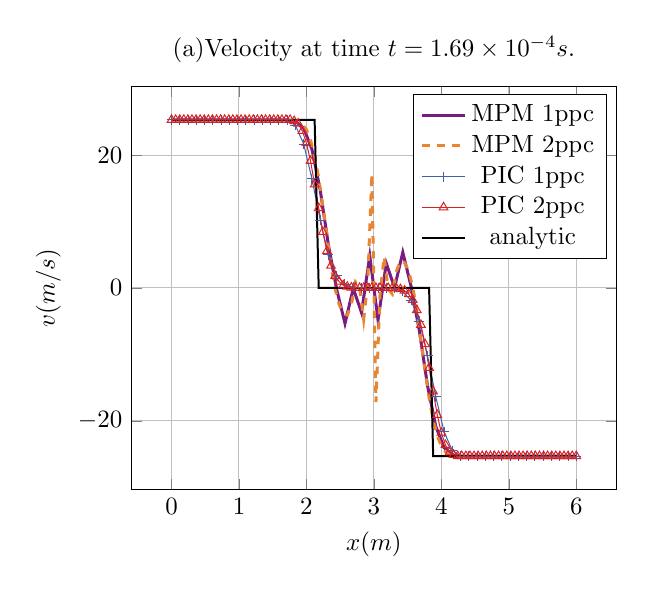
\begin{tikzpicture}[scale=0.9]
\begin{axis}[xlabel=$x (m)$,ylabel=$v (m/s)$,ymajorgrids=true,xmajorgrids=true,title={(a)Velocity at time $t=1.69\times 10^{-4}s.$}]
\addplot[Purple,very thick,mark=none,solid] coordinates {(0.0,25.3184841771) (0.122448979592,25.3184841771) (0.244897959184,25.3184841771) (0.367346938776,25.3184841771) (0.489795918367,25.3184841771) (0.612244897959,25.3184841771) (0.734693877551,25.3184841771) (0.857142857143,25.3184841771) (0.979591836735,25.3184841771) (1.10204081633,25.3184841771) (1.22448979592,25.3184841771) (1.34693877551,25.3184841771) (1.4693877551,25.3184841771) (1.59183673469,25.3184841771) (1.71428571429,25.3184841771) (1.83673469388,25.1149797615) (1.95918367347,24.0545424864) (2.08163265306,20.8743509476) (2.20408163265,14.7547033581) (2.32653061224,6.41598558277) (2.44897959184,-0.244456370035) (2.57142857143,-5.35821612759) (2.69387755102,-0.0619763112976) (2.81632653061,-3.709401685) (2.9387755102,4.8348853161) (3.0612244898,-4.8348853161) (3.18367346939,3.709401685) (3.30612244898,0.0619763112976) (3.42857142857,5.35821612759) (3.55102040816,0.244456370035) (3.67346938776,-6.41598558277) (3.79591836735,-14.7547033581) (3.91836734694,-20.8743509476) (4.04081632653,-24.0545424864) (4.16326530612,-25.1149797615) (4.28571428571,-25.3184841771) (4.40816326531,-25.3184841771) (4.5306122449,-25.3184841771) (4.65306122449,-25.3184841771) (4.77551020408,-25.3184841771) (4.89795918367,-25.3184841771) (5.02040816327,-25.3184841771) (5.14285714286,-25.3184841771) (5.26530612245,-25.3184841771) (5.38775510204,-25.3184841771) (5.51020408163,-25.3184841771) (5.63265306122,-25.3184841771) (5.75510204082,-25.3184841771) (5.87755102041,-25.3184841771) (6.0,-25.3184841771) };
\addplot[Orange,very thick,mark=none,dashed] coordinates {(0.0,25.3184841771) (0.0606060606061,25.3184841771) (0.121212121212,25.3184841771) (0.181818181818,25.3184841771) (0.242424242424,25.3184841771) (0.30303030303,25.3184841771) (0.363636363636,25.3184841771) (0.424242424242,25.3184841771) (0.484848484848,25.3184841771) (0.545454545455,25.3184841771) (0.606060606061,25.3184841771) (0.666666666667,25.3184841771) (0.727272727273,25.3184841771) (0.787878787879,25.3184841771) (0.848484848485,25.3184841771) (0.909090909091,25.3184841771) (0.969696969697,25.3184841771) (1.0303030303,25.3184841771) (1.09090909091,25.3184841771) (1.15151515152,25.3184841771) (1.21212121212,25.3184841771) (1.27272727273,25.3184841771) (1.33333333333,25.3184841771) (1.39393939394,25.3184841771) (1.45454545455,25.3184841771) (1.51515151515,25.3184841771) (1.57575757576,25.3184841771) (1.63636363636,25.3184841771) (1.69696969697,25.3184841771) (1.75757575758,25.3184841771) (1.81818181818,25.251933876) (1.87878787879,25.1188332739) (1.93939393939,24.6493504882) (2.0,23.8434855187) (2.06060606061,22.247450502) (2.12121212121,19.8612454379) (2.18181818182,16.5614104839) (2.24242424242,12.3479456399) (2.30303030303,7.94379399222) (2.36363636364,3.34895554082) (2.42424242424,-0.133198996542) (2.48484848485,-2.50266961986) (2.54545454545,-3.82041358095) (2.60606060606,-4.08643087983) (2.66666666667,-2.50894819569) (2.72727272727,0.91203447147) (2.78787878788,0.178185932665) (2.84848484848,-4.71049381211) (2.90909090909,0.963495780905) (2.9696969697,17.2001547117) (3.0303030303,-17.2001547117) (3.09090909091,-0.963495780905) (3.15151515152,4.7104938121) (3.21212121212,-0.178185932665) (3.27272727273,-0.91203447147) (3.33333333333,2.50894819569) (3.39393939394,4.08643087983) (3.45454545455,3.82041358095) (3.51515151515,2.50266961986) (3.57575757576,0.133198996542) (3.63636363636,-3.34895554082) (3.69696969697,-7.94379399222) (3.75757575758,-12.3479456399) (3.81818181818,-16.5614104839) (3.87878787879,-19.8612454379) (3.93939393939,-22.247450502) (4.0,-23.8434855187) (4.06060606061,-24.6493504882) (4.12121212121,-25.1188332739) (4.18181818182,-25.251933876) (4.24242424242,-25.3184841771) (4.30303030303,-25.3184841771) (4.36363636364,-25.3184841771) (4.42424242424,-25.3184841771) (4.48484848485,-25.3184841771) (4.54545454545,-25.3184841771) (4.60606060606,-25.3184841771) (4.66666666667,-25.3184841771) (4.72727272727,-25.3184841771) (4.78787878788,-25.3184841771) (4.84848484848,-25.3184841771) (4.90909090909,-25.3184841771) (4.9696969697,-25.3184841771) (5.0303030303,-25.3184841771) (5.09090909091,-25.3184841771) (5.15151515152,-25.3184841771) (5.21212121212,-25.3184841771) (5.27272727273,-25.3184841771) (5.33333333333,-25.3184841771) (5.39393939394,-25.3184841771) (5.45454545455,-25.3184841771) (5.51515151515,-25.3184841771) (5.57575757576,-25.3184841771) (5.63636363636,-25.3184841771) (5.69696969697,-25.3184841771) (5.75757575758,-25.3184841771) (5.81818181818,-25.3184841771) (5.87878787879,-25.3184841771) (5.93939393939,-25.3184841771) (6.0,-25.3184841771) };
\addplot[Blue,thin,mark=+,solid] coordinates {(0.0,25.3184841771) (0.122448979592,25.3184841771) (0.244897959184,25.3184841771) (0.367346938776,25.3184841771) (0.489795918367,25.3184841771) (0.612244897959,25.3184841771) (0.734693877551,25.3184841771) (0.857142857143,25.3184841771) (0.979591836735,25.3184841771) (1.10204081633,25.3184841771) (1.22448979592,25.3184841771) (1.34693877551,25.3184841771) (1.4693877551,25.3184841771) (1.59183673469,25.3184841771) (1.71428571429,25.3184841771) (1.83673469388,24.4761330084) (1.95918367347,21.6789610487) (2.08163265306,16.4171127559) (2.20408163265,10.2176854187) (2.32653061224,4.99697293397) (2.44897959184,1.87425322807) (2.57142857143,0.532987126345) (2.69387755102,0.0744368580376) (2.81632653061,0.0446687900239) (2.9387755102,-0.0367040274884) (3.0612244898,0.0367040274884) (3.18367346939,-0.0446687900239) (3.30612244898,-0.0744368580376) (3.42857142857,-0.532987126345) (3.55102040816,-1.87425322807) (3.67346938776,-4.99697293397) (3.79591836735,-10.2176854187) (3.91836734694,-16.4171127559) (4.04081632653,-21.6789610487) (4.16326530612,-24.4761330084) (4.28571428571,-25.3184841771) (4.40816326531,-25.3184841771) (4.5306122449,-25.3184841771) (4.65306122449,-25.3184841771) (4.77551020408,-25.3184841771) (4.89795918367,-25.3184841771) (5.02040816327,-25.3184841771) (5.14285714286,-25.3184841771) (5.26530612245,-25.3184841771) (5.38775510204,-25.3184841771) (5.51020408163,-25.3184841771) (5.63265306122,-25.3184841771) (5.75510204082,-25.3184841771) (5.87755102041,-25.3184841771) (6.0,-25.3184841771) };
\addplot[Red,thin,mark=triangle,solid] coordinates {(0.0,25.3184841771) (0.0606060606061,25.3184841771) (0.121212121212,25.3184841771) (0.181818181818,25.3184841771) (0.242424242424,25.3184841771) (0.30303030303,25.3184841771) (0.363636363636,25.3184841771) (0.424242424242,25.3184841771) (0.484848484848,25.3184841771) (0.545454545455,25.3184841771) (0.606060606061,25.3184841771) (0.666666666667,25.3184841771) (0.727272727273,25.3184841771) (0.787878787879,25.3184841771) (0.848484848485,25.3184841771) (0.909090909091,25.3184841771) (0.969696969697,25.3184841771) (1.0303030303,25.3184841771) (1.09090909091,25.3184841771) (1.15151515152,25.3184841771) (1.21212121212,25.3184841771) (1.27272727273,25.3184841771) (1.33333333333,25.3184841771) (1.39393939394,25.3184841771) (1.45454545455,25.3184841771) (1.51515151515,25.3184841771) (1.57575757576,25.3184841771) (1.63636363636,25.3184841771) (1.69696969697,25.3184841771) (1.75757575758,25.3184841771) (1.81818181818,25.1281304409) (1.87878787879,24.7474229685) (1.93939393939,23.6387415979) (2.0,21.8020863292) (2.06060606061,19.1201129846) (2.12121212121,15.5928215642) (2.18181818182,12.0349431808) (2.24242424242,8.44647783432) (2.30303030303,5.5505820269) (2.36363636364,3.3472557585) (2.42424242424,1.81296030454) (2.48484848485,0.947695665037) (2.54545454545,0.405594826726) (2.60606060606,0.186657789609) (2.66666666667,0.0594742699364) (2.72727272727,0.0240442677077) (2.78787878788,0.00485504304949) (2.84848484848,0.00190659596188) (2.90909090909,0.000324279313551) (2.9696969697,0.000108093104517) (3.0303030303,-0.000108093104518) (3.09090909091,-0.000324279313554) (3.15151515152,-0.00190659596188) (3.21212121212,-0.0048550430495) (3.27272727273,-0.0240442677077) (3.33333333333,-0.0594742699364) (3.39393939394,-0.186657789609) (3.45454545455,-0.405594826726) (3.51515151515,-0.947695665037) (3.57575757576,-1.81296030454) (3.63636363636,-3.3472557585) (3.69696969697,-5.5505820269) (3.75757575758,-8.44647783432) (3.81818181818,-12.0349431808) (3.87878787879,-15.5928215642) (3.93939393939,-19.1201129846) (4.0,-21.8020863292) (4.06060606061,-23.6387415979) (4.12121212121,-24.7474229685) (4.18181818182,-25.1281304409) (4.24242424242,-25.3184841771) (4.30303030303,-25.3184841771) (4.36363636364,-25.3184841771) (4.42424242424,-25.3184841771) (4.48484848485,-25.3184841771) (4.54545454545,-25.3184841771) (4.60606060606,-25.3184841771) (4.66666666667,-25.3184841771) (4.72727272727,-25.3184841771) (4.78787878788,-25.3184841771) (4.84848484848,-25.3184841771) (4.90909090909,-25.3184841771) (4.9696969697,-25.3184841771) (5.0303030303,-25.3184841771) (5.09090909091,-25.3184841771) (5.15151515152,-25.3184841771) (5.21212121212,-25.3184841771) (5.27272727273,-25.3184841771) (5.33333333333,-25.3184841771) (5.39393939394,-25.3184841771) (5.45454545455,-25.3184841771) (5.51515151515,-25.3184841771) (5.57575757576,-25.3184841771) (5.63636363636,-25.3184841771) (5.69696969697,-25.3184841771) (5.75757575758,-25.3184841771) (5.81818181818,-25.3184841771) (5.87878787879,-25.3184841771) (5.93939393939,-25.3184841771) (6.0,-25.3184841771) };
\addplot[black,thick,mark=none,solid] coordinates {(0.0,25.3184841771) (0.0606060606061,25.3184841771) (0.121212121212,25.3184841771) (0.181818181818,25.3184841771) (0.242424242424,25.3184841771) (0.30303030303,25.3184841771) (0.363636363636,25.3184841771) (0.424242424242,25.3184841771) (0.484848484848,25.3184841771) (0.545454545455,25.3184841771) (0.606060606061,25.3184841771) (0.666666666667,25.3184841771) (0.727272727273,25.3184841771) (0.787878787879,25.3184841771) (0.848484848485,25.3184841771) (0.909090909091,25.3184841771) (0.969696969697,25.3184841771) (1.0303030303,25.3184841771) (1.09090909091,25.3184841771) (1.15151515152,25.3184841771) (1.21212121212,25.3184841771) (1.27272727273,25.3184841771) (1.33333333333,25.3184841771) (1.39393939394,25.3184841771) (1.45454545455,25.3184841771) (1.51515151515,25.3184841771) (1.57575757576,25.3184841771) (1.63636363636,25.3184841771) (1.69696969697,25.3184841771) (1.75757575758,25.3184841771) (1.81818181818,25.3184841771) (1.87878787879,25.3184841771) (1.93939393939,25.3184841771) (2.0,25.3184841771) (2.06060606061,25.3184841771) (2.12121212121,25.3184841771) (2.18181818182,0.0) (2.24242424242,0.0) (2.30303030303,0.0) (2.36363636364,0.0) (2.42424242424,0.0) (2.48484848485,0.0) (2.54545454545,0.0) (2.60606060606,0.0) (2.66666666667,0.0) (2.72727272727,0.0) (2.78787878788,0.0) (2.84848484848,0.0) (2.90909090909,0.0) (2.9696969697,0.0) (3.0303030303,-0.0) (3.09090909091,-0.0) (3.15151515152,-0.0) (3.21212121212,-0.0) (3.27272727273,-0.0) (3.33333333333,-0.0) (3.39393939394,-0.0) (3.45454545455,-0.0) (3.51515151515,-0.0) (3.57575757576,-0.0) (3.63636363636,-0.0) (3.69696969697,-0.0) (3.75757575758,-0.0) (3.81818181818,-0.0) (3.87878787879,-25.3184841771) (3.93939393939,-25.3184841771) (4.0,-25.3184841771) (4.06060606061,-25.3184841771) (4.12121212121,-25.3184841771) (4.18181818182,-25.3184841771) (4.24242424242,-25.3184841771) (4.30303030303,-25.3184841771) (4.36363636364,-25.3184841771) (4.42424242424,-25.3184841771) (4.48484848485,-25.3184841771) (4.54545454545,-25.3184841771) (4.60606060606,-25.3184841771) (4.66666666667,-25.3184841771) (4.72727272727,-25.3184841771) (4.78787878788,-25.3184841771) (4.84848484848,-25.3184841771) (4.90909090909,-25.3184841771) (4.9696969697,-25.3184841771) (5.0303030303,-25.3184841771) (5.09090909091,-25.3184841771) (5.15151515152,-25.3184841771) (5.21212121212,-25.3184841771) (5.27272727273,-25.3184841771) (5.33333333333,-25.3184841771) (5.39393939394,-25.3184841771) (5.45454545455,-25.3184841771) (5.51515151515,-25.3184841771) (5.57575757576,-25.3184841771) (5.63636363636,-25.3184841771) (5.69696969697,-25.3184841771) (5.75757575758,-25.3184841771) (5.81818181818,-25.3184841771) (5.87878787879,-25.3184841771) (5.93939393939,-25.3184841771) (6.0,-25.3184841771) };
\legend{MPM 1ppc,MPM 2ppc,PIC 1ppc,PIC 2ppc,analytic}
\end{axis}
\end{tikzpicture}
%%% Local Variables: 
%%% mode: latex
%%% TeX-master: "../../mainManuscript"
%%% End:
\phantomsubcaption \label{subfig:MPM_velo_10}}
  {\definecolor{Purple}{RGB}{120,28,129}
\definecolor{Orange}{RGB}{231,133,50}
\definecolor{Blue}{RGB}{63,96,174}
\definecolor{Red}{RGB}{217,33,32}
\definecolor{Duck}{RGB}{83,158,182}
\definecolor{Green}{RGB}{109,179,136}
\definecolor{Yellow}{RGB}{202,184,67}
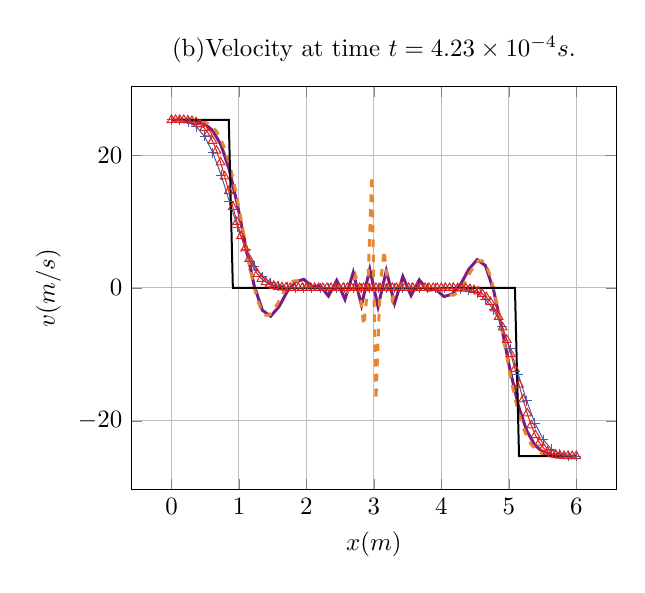
\begin{tikzpicture}[scale=0.9]
\begin{axis}[xlabel=$x (m)$,ylabel=$v (m/s)$,ymajorgrids=true,xmajorgrids=true,title={(b)Velocity at time $t=4.23\times 10^{-4}s.$}]
\addplot[Purple,very thick,mark=none,solid] coordinates {(0.0,25.3179577559) (0.122448979592,25.3125244526) (0.244897959184,25.2804932478) (0.367346938776,25.1489907367) (0.489795918367,24.7341796044) (0.612244897959,23.6864809647) (0.734693877551,21.5118739395) (0.857142857143,17.7671095652) (0.979591836735,12.4121755247) (1.10204081633,6.14683940753) (1.22448979592,0.373716046882) (1.34693877551,-3.3616057723) (1.4693877551,-4.26176674269) (1.59183673469,-2.83406587609) (1.71428571429,-0.55562049587) (1.83673469388,0.901404345798) (1.95918367347,1.30403292578) (2.08163265306,0.214501074535) (2.20408163265,0.352209313776) (2.32653061224,-1.21718822558) (2.44897959184,1.14054029809) (2.57142857143,-1.72149525556) (2.69387755102,2.335373076) (2.81632653061,-2.59610029814) (2.9387755102,2.82071480229) (3.0612244898,-2.82071480229) (3.18367346939,2.59610029814) (3.30612244898,-2.335373076) (3.42857142857,1.72149525556) (3.55102040816,-1.14054029809) (3.67346938776,1.21718822558) (3.79591836735,-0.352209313776) (3.91836734694,-0.214501074535) (4.04081632653,-1.30403292578) (4.16326530612,-0.901404345798) (4.28571428571,0.55562049587) (4.40816326531,2.83406587609) (4.5306122449,4.26176674269) (4.65306122449,3.3616057723) (4.77551020408,-0.373716046882) (4.89795918367,-6.14683940753) (5.02040816327,-12.4121755247) (5.14285714286,-17.7671095652) (5.26530612245,-21.5118739395) (5.38775510204,-23.6864809647) (5.51020408163,-24.7341796044) (5.63265306122,-25.1489907367) (5.75510204082,-25.2804932478) (5.87755102041,-25.3125244526) (6.0,-25.3179577559) };
\addplot[Orange,very thick,mark=none,dashed] coordinates {(0.0,25.3184113784) (0.0606060606061,25.3182657812) (0.121212121212,25.3171343813) (0.181818181818,25.3150171787) (0.242424242424,25.3062460446) (0.30303030303,25.2908209787) (0.363636363636,25.2461773758) (0.424242424242,25.1723152357) (0.484848484848,25.0062868064) (0.545454545455,24.748092088) (0.606060606061,24.2720385643) (0.666666666667,23.5781262352) (0.727272727273,22.4951335769) (0.787878787879,21.0230605893) (0.848484848485,19.0428242456) (0.909090909091,16.5544245458) (0.969696969697,13.6460768618) (1.0303030303,10.3177811934) (1.09090909091,6.94923058708) (1.15151515152,3.54042504293) (1.21212121212,0.626561316633) (1.27272727273,-1.79236059183) (1.33333333333,-3.36301978655) (1.39393939394,-4.08541626753) (1.45454545455,-4.06554257142) (1.51515151515,-3.30339869822) (1.57575757576,-2.29577774705) (1.63636363636,-1.04267971791) (1.69696969697,-0.0393881478233) (1.75757575758,0.714096963215) (1.81818181818,1.07591385411) (1.87878787879,1.04606252486) (1.93939393939,0.832069940855) (2.0,0.433936102092) (2.06060606061,0.100491892604) (2.12121212121,-0.168262687611) (2.18181818182,-0.281962807299) (2.24242424242,-0.24060846646) (2.30303030303,-0.19473430746) (2.36363636364,-0.144340330301) (2.42424242424,0.0103021847971) (2.48484848485,0.269193237834) (2.54545454545,0.0743373654573) (2.60606060606,-0.574265432333) (2.66666666667,0.0252212025898) (2.72727272727,1.87279727022) (2.78787878788,-0.017779131944) (2.84848484848,-5.64650800392) (2.90909090909,-0.0160332856532) (2.9696969697,16.8736450228) (3.0303030303,-16.8736450228) (3.09090909091,0.0160332856532) (3.15151515152,5.64650800392) (3.21212121212,0.017779131944) (3.27272727273,-1.87279727022) (3.33333333333,-0.0252212025898) (3.39393939394,0.574265432333) (3.45454545455,-0.0743373654573) (3.51515151515,-0.269193237834) (3.57575757576,-0.0103021847971) (3.63636363636,0.144340330301) (3.69696969697,0.19473430746) (3.75757575758,0.24060846646) (3.81818181818,0.281962807299) (3.87878787879,0.168262687611) (3.93939393939,-0.100491892604) (4.0,-0.433936102092) (4.06060606061,-0.832069940855) (4.12121212121,-1.04606252486) (4.18181818182,-1.07591385411) (4.24242424242,-0.714096963215) (4.30303030303,0.0393881478233) (4.36363636364,1.04267971791) (4.42424242424,2.29577774705) (4.48484848485,3.30339869822) (4.54545454545,4.06554257142) (4.60606060606,4.08541626753) (4.66666666667,3.36301978655) (4.72727272727,1.79236059183) (4.78787878788,-0.626561316633) (4.84848484848,-3.54042504293) (4.90909090909,-6.94923058708) (4.9696969697,-10.3177811934) (5.0303030303,-13.6460768618) (5.09090909091,-16.5544245458) (5.15151515152,-19.0428242456) (5.21212121212,-21.0230605893) (5.27272727273,-22.4951335769) (5.33333333333,-23.5781262352) (5.39393939394,-24.2720385643) (5.45454545455,-24.748092088) (5.51515151515,-25.0062868064) (5.57575757576,-25.1723152357) (5.63636363636,-25.2461773758) (5.69696969697,-25.2908209787) (5.75757575758,-25.3062460446) (5.81818181818,-25.3150171787) (5.87878787879,-25.3171343813) (5.93939393939,-25.3182657812) (6.0,-25.3184113784) };
\addplot[Blue,thin,mark=+,solid] coordinates {(0.0,25.3092803388) (0.122448979592,25.2447324562) (0.244897959184,24.9883092861) (0.367346938776,24.2884039338) (0.489795918367,22.8251885418) (0.612244897959,20.3815104479) (0.734693877551,17.0009533921) (0.857142857143,13.0691188281) (0.979591836735,9.15154944222) (1.10204081633,5.79708129579) (1.22448979592,3.29261988393) (1.34693877551,1.675771205) (1.4693877551,0.752811727213) (1.59183673469,0.303721307352) (1.71428571429,0.103656250171) (1.83673469388,0.0339292027744) (1.95918367347,0.00764630747691) (2.08163265306,0.00206351249066) (2.20408163265,0.00116478529579) (2.32653061224,-0.00170580325334) (2.44897959184,0.00273380703211) (2.57142857143,-0.00360718467272) (2.69387755102,0.00434097653714) (2.81632653061,-0.00486620536301) (2.9387755102,0.00514034587123) (3.0612244898,-0.00514034587123) (3.18367346939,0.004866205363) (3.30612244898,-0.00434097653715) (3.42857142857,0.00360718467272) (3.55102040816,-0.00273380703212) (3.67346938776,0.00170580325334) (3.79591836735,-0.0011647852958) (3.91836734694,-0.00206351249067) (4.04081632653,-0.00764630747693) (4.16326530612,-0.0339292027744) (4.28571428571,-0.103656250171) (4.40816326531,-0.303721307352) (4.5306122449,-0.752811727213) (4.65306122449,-1.675771205) (4.77551020408,-3.29261988393) (4.89795918367,-5.79708129579) (5.02040816327,-9.15154944222) (5.14285714286,-13.0691188281) (5.26530612245,-17.0009533921) (5.38775510204,-20.3815104479) (5.51020408163,-22.8251885418) (5.63265306122,-24.2884039338) (5.75510204082,-24.9883092861) (5.87755102041,-25.2447324562) (6.0,-25.3092803388) };
\addplot[Red,thin,mark=triangle,solid] coordinates {(0.0,25.317930571) (0.0606060606061,25.3168233587) (0.121212121212,25.309085386) (0.181818181818,25.2947166528) (0.242424242424,25.244614182) (0.30303030303,25.1587779735) (0.363636363636,24.9586620152) (0.424242424242,24.6442663072) (0.484848484848,24.0900542943) (0.545454545455,23.2960259765) (0.606060606061,22.1613724279) (0.666666666667,20.6860936486) (0.727272727273,18.8976424995) (0.787878787879,16.7960189808) (0.848484848485,14.5640565488) (0.909090909091,12.2017552037) (0.969696969697,9.95104414047) (1.0303030303,7.81192335918) (1.09090909091,5.95010149482) (1.15151515152,4.3655785474) (1.21212121212,3.08784304074) (1.27272727273,2.11689497486) (1.33333333333,1.38335842096) (1.39393939394,0.887233379031) (1.45454545455,0.532919503373) (1.51515151515,0.320416793985) (1.57575757576,0.175908565338) (1.63636363636,0.099394817433) (1.69696969697,0.0495526747861) (1.75757575758,0.0263821373972) (1.81818181818,0.0118516742131) (1.87878787879,0.00596128523387) (1.93939393939,0.00239032827724) (2.0,0.00113880334319) (2.06060606061,0.000402762467656) (2.12121212121,0.000182205650641) (2.18181818182,5.59845952697e-05) (2.24242424242,2.40993015427e-05) (2.30303030303,6.30122659209e-06) (2.36363636364,2.59037041785e-06) (2.42424242424,5.63023256661e-07) (2.48484848485,2.19185108534e-07) (2.54545454545,3.6441322259e-08) (2.60606060606,1.47918978351e-08) (2.66666666667,2.77206499505e-09) (2.72727272727,3.8182373896e-10) (2.78787878788,-5.09485431597e-10) (2.84848484848,9.81374833763e-11) (2.90909090909,3.01460955695e-10) (2.9696969697,1.0048498536e-10) (3.0303030303,-1.00489619785e-10) (3.09090909091,-3.01462859741e-10) (3.15151515152,-9.81387986931e-11) (3.21212121212,5.0948256336e-10) (3.27272727273,-3.81824116856e-10) (3.33333333333,-2.77205883934e-09) (3.39393939394,-1.47918917763e-08) (3.45454545455,-3.64413229276e-08) (3.51515151515,-2.19185109959e-07) (3.57575757576,-5.6302325287e-07) (3.63636363636,-2.59037041421e-06) (3.69696969697,-6.30122659398e-06) (3.75757575758,-2.40993015444e-05) (3.81818181818,-5.59845952656e-05) (3.87878787879,-0.000182205650636) (3.93939393939,-0.000402762467656) (4.0,-0.00113880334319) (4.06060606061,-0.00239032827724) (4.12121212121,-0.00596128523387) (4.18181818182,-0.0118516742131) (4.24242424242,-0.0263821373972) (4.30303030303,-0.0495526747861) (4.36363636364,-0.099394817433) (4.42424242424,-0.175908565338) (4.48484848485,-0.320416793985) (4.54545454545,-0.532919503373) (4.60606060606,-0.887233379031) (4.66666666667,-1.38335842096) (4.72727272727,-2.11689497486) (4.78787878788,-3.08784304074) (4.84848484848,-4.3655785474) (4.90909090909,-5.95010149482) (4.9696969697,-7.81192335918) (5.0303030303,-9.95104414047) (5.09090909091,-12.2017552037) (5.15151515152,-14.5640565488) (5.21212121212,-16.7960189808) (5.27272727273,-18.8976424995) (5.33333333333,-20.6860936486) (5.39393939394,-22.1613724279) (5.45454545455,-23.2960259765) (5.51515151515,-24.0900542943) (5.57575757576,-24.6442663072) (5.63636363636,-24.9586620152) (5.69696969697,-25.1587779735) (5.75757575758,-25.244614182) (5.81818181818,-25.2947166528) (5.87878787879,-25.309085386) (5.93939393939,-25.3168233587) (6.0,-25.317930571) };
\addplot[black,thick,mark=none,solid] coordinates {(0.0,25.3184841771) (0.0606060606061,25.3184841771) (0.121212121212,25.3184841771) (0.181818181818,25.3184841771) (0.242424242424,25.3184841771) (0.30303030303,25.3184841771) (0.363636363636,25.3184841771) (0.424242424242,25.3184841771) (0.484848484848,25.3184841771) (0.545454545455,25.3184841771) (0.606060606061,25.3184841771) (0.666666666667,25.3184841771) (0.727272727273,25.3184841771) (0.787878787879,25.3184841771) (0.848484848485,25.3184841771) (0.909090909091,0.0) (0.969696969697,0.0) (1.0303030303,0.0) (1.09090909091,0.0) (1.15151515152,0.0) (1.21212121212,0.0) (1.27272727273,0.0) (1.33333333333,0.0) (1.39393939394,0.0) (1.45454545455,0.0) (1.51515151515,0.0) (1.57575757576,0.0) (1.63636363636,0.0) (1.69696969697,0.0) (1.75757575758,0.0) (1.81818181818,0.0) (1.87878787879,0.0) (1.93939393939,0.0) (2.0,0.0) (2.06060606061,0.0) (2.12121212121,0.0) (2.18181818182,0.0) (2.24242424242,0.0) (2.30303030303,0.0) (2.36363636364,0.0) (2.42424242424,0.0) (2.48484848485,0.0) (2.54545454545,0.0) (2.60606060606,0.0) (2.66666666667,0.0) (2.72727272727,0.0) (2.78787878788,0.0) (2.84848484848,0.0) (2.90909090909,0.0) (2.9696969697,0.0) (3.0303030303,-0.0) (3.09090909091,-0.0) (3.15151515152,-0.0) (3.21212121212,-0.0) (3.27272727273,-0.0) (3.33333333333,-0.0) (3.39393939394,-0.0) (3.45454545455,-0.0) (3.51515151515,-0.0) (3.57575757576,-0.0) (3.63636363636,-0.0) (3.69696969697,-0.0) (3.75757575758,-0.0) (3.81818181818,-0.0) (3.87878787879,-0.0) (3.93939393939,-0.0) (4.0,-0.0) (4.06060606061,-0.0) (4.12121212121,-0.0) (4.18181818182,-0.0) (4.24242424242,-0.0) (4.30303030303,-0.0) (4.36363636364,-0.0) (4.42424242424,-0.0) (4.48484848485,-0.0) (4.54545454545,-0.0) (4.60606060606,-0.0) (4.66666666667,-0.0) (4.72727272727,-0.0) (4.78787878788,-0.0) (4.84848484848,-0.0) (4.90909090909,-0.0) (4.9696969697,-0.0) (5.0303030303,-0.0) (5.09090909091,-0.0) (5.15151515152,-25.3184841771) (5.21212121212,-25.3184841771) (5.27272727273,-25.3184841771) (5.33333333333,-25.3184841771) (5.39393939394,-25.3184841771) (5.45454545455,-25.3184841771) (5.51515151515,-25.3184841771) (5.57575757576,-25.3184841771) (5.63636363636,-25.3184841771) (5.69696969697,-25.3184841771) (5.75757575758,-25.3184841771) (5.81818181818,-25.3184841771) (5.87878787879,-25.3184841771) (5.93939393939,-25.3184841771) (6.0,-25.3184841771) };
%\legend{USL 1ppc,USL 2ppc,PIC 1ppc,PIC 2ppc,analytic}
\end{axis}
\end{tikzpicture}
%%% Local Variables: 
%%% mode: latex
%%% TeX-master: "../../mainManuscript"
%%% End:
\phantomsubcaption \label{subfig:MPM_velo_25}}
  \caption{Comparison between USL algorithm with classical or PIC mapping and exact velocities of the bars impact problem for various discretizations.}
  \label{fig:MPM_velocities}
\end{figure}
Thus, the PIC projection \eqref{eq:PIC_Back-mapping} has been implemented into the USL formulation in order to compare it to the original USL algorithm and to the exact solution (figures \ref{fig:MPM_velocities}\subref{subfig:MPM_velo_10} and \ref{fig:MPM_velocities}\subref{subfig:MPM_velo_10}). As can be seen, the introduction of the PIC projection enables the elimination of noise in the numerical solution as well as the "locking" of the velocity in the middle region of the bar. Hence, the modified USL shows a good agreement with the exact solution in terms of velocity and stress (see figures \ref{fig:mpm_diffusion}\subref{subfig:mpm_diffusion_10} and \ref{fig:mpm_diffusion}\subref{subfig:mpm_diffusion_25}). Nevertheless, the modified USL is more diffusive, as shown in figure \ref{fig:mpm_diffusion}\subref{subfig:mpm_energies}. This result was expected since the PIC projection step was removed in order to reduce the numerical dissipation \cite{PIC_Nishiguchi}. 
\begin{figure}[h!]
  \centering
  {\definecolor{Purple}{RGB}{120,28,129}
\definecolor{Orange}{RGB}{231,133,50}
\definecolor{Blue}{RGB}{63,96,174}
\definecolor{Red}{RGB}{217,33,32}
\definecolor{Duck}{RGB}{83,158,182}
\definecolor{Green}{RGB}{109,179,136}
\definecolor{Yellow}{RGB}{202,184,67}
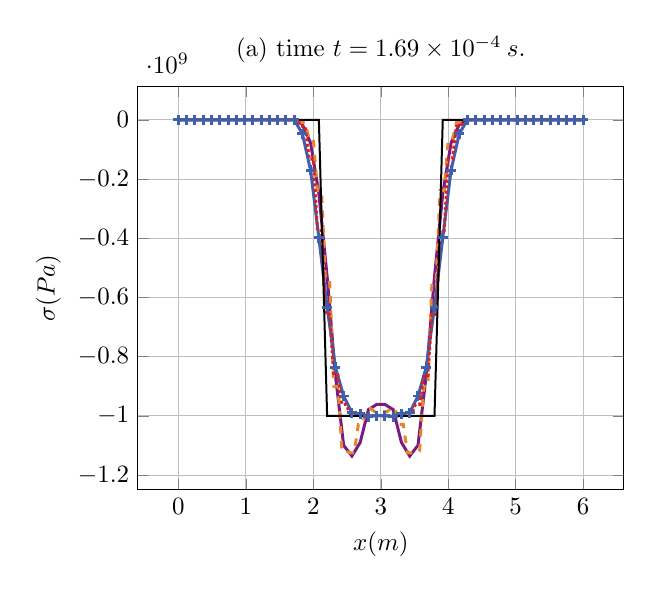
\begin{tikzpicture}[scale=0.9]
\begin{axis}[xlabel=$x (m)$,ylabel=$\sigma (Pa)$,ymajorgrids=true,xmajorgrids=true,title={(a) time $t=1.69\times 10^{-4}\: s.$}]
\addplot[Purple,very thick,mark=none,solid] coordinates {(0.0,-9.62200780097e-08) (0.122448979592,-1.92440156019e-07) (0.244897959184,-9.62200780097e-08) (0.367346938776,0.0) (0.489795918367,9.62200780097e-08) (0.612244897959,-9.62200780097e-08) (0.734693877551,-1.92440156019e-07) (0.857142857143,-9.62200780097e-08) (0.979591836735,-9.62200780097e-08) (1.10204081633,0.0) (1.22448979592,9.62200780097e-08) (1.34693877551,-9.62200780097e-08) (1.4693877551,0.0) (1.59183673469,0.0) (1.71428571429,0.0) (1.83673469388,-15437652.4848) (1.95918367347,-78183137.9185) (2.08163265306,-249067223.585) (2.20408163265,-529536815.675) (2.32653061224,-862202048.46) (2.44897959184,-1099498863.41) (2.57142857143,-1135789315.44) (2.69387755102,-1090007223.73) (2.81632653061,-978780358.738) (2.9387755102,-961497360.562) (3.0612244898,-961497360.562) (3.18367346939,-978780358.738) (3.30612244898,-1090007223.73) (3.42857142857,-1135789315.44) (3.55102040816,-1099498863.41) (3.67346938776,-862202048.46) (3.79591836735,-529536815.675) (3.91836734694,-249067223.585) (4.04081632653,-78183137.9185) (4.16326530612,-15437652.4848) (4.28571428571,-3.85185988877e-23) (4.40816326531,-9.62200780097e-08) (4.5306122449,9.62200780097e-08) (4.65306122449,9.62200780097e-08) (4.77551020408,9.62200780097e-08) (4.89795918367,-2.88660234029e-07) (5.02040816327,-9.62200780097e-08) (5.14285714286,9.62200780097e-08) (5.26530612245,1.92440156019e-07) (5.38775510204,2.88660234029e-07) (5.51020408163,9.62200780097e-08) (5.63265306122,0.0) (5.75510204082,0.0) (5.87755102041,0.0) (6.0,-9.62200780097e-08) };
\addplot[Orange,very thick,mark=none,dashed] coordinates {(0.0,0.0) (0.0606060606061,0.0) (0.121212121212,9.52481580298e-08) (0.181818181818,9.52481580298e-08) (0.242424242424,9.52481580298e-08) (0.30303030303,9.52481580298e-08) (0.363636363636,0.0) (0.424242424242,0.0) (0.484848484848,-9.52481580298e-08) (0.545454545455,-9.52481580298e-08) (0.606060606061,-1.9049631606e-07) (0.666666666667,-1.9049631606e-07) (0.727272727273,0.0) (0.787878787879,0.0) (0.848484848485,0.0) (0.909090909091,0.0) (0.969696969697,-3.85185988877e-23) (1.0303030303,-3.85185988877e-23) (1.09090909091,-9.52481580298e-08) (1.15151515152,-9.52481580298e-08) (1.21212121212,9.52481580298e-08) (1.27272727273,9.52481580298e-08) (1.33333333333,9.52481580298e-08) (1.39393939394,9.52481580298e-08) (1.45454545455,-1.9049631606e-07) (1.51515151515,-1.9049631606e-07) (1.57575757576,1.9049631606e-07) (1.63636363636,1.9049631606e-07) (1.69696969697,0.0) (1.75757575758,0.0) (1.81818181818,-9533923.2537) (1.87878787879,-9533923.2537) (1.93939393939,-67166647.336) (2.0,-67166647.336) (2.06060606061,-239339979.822) (2.12121212121,-239339979.822) (2.18181818182,-549695480.518) (2.24242424242,-549695480.518) (2.30303030303,-900240202.504) (2.36363636364,-900240202.504) (2.42424242424,-1118552245.0) (2.48484848485,-1118552245.0) (2.54545454545,-1125362633.2) (2.60606060606,-1125362633.2) (2.66666666667,-1028724363.35) (2.72727272727,-1028724363.35) (2.78787878788,-975375246.836) (2.84848484848,-975375246.836) (2.90909090909,-986009278.185) (2.9696969697,-986009278.185) (3.0303030303,-986009278.185) (3.09090909091,-986009278.185) (3.15151515152,-975375246.836) (3.21212121212,-975375246.836) (3.27272727273,-1028724363.35) (3.33333333333,-1028724363.35) (3.39393939394,-1125362633.2) (3.45454545455,-1125362633.2) (3.51515151515,-1118552245.0) (3.57575757576,-1118552245.0) (3.63636363636,-900240202.504) (3.69696969697,-900240202.504) (3.75757575758,-549695480.518) (3.81818181818,-549695480.518) (3.87878787879,-239339979.822) (3.93939393939,-239339979.822) (4.0,-67166647.336) (4.06060606061,-67166647.336) (4.12121212121,-9533923.2537) (4.18181818182,-9533923.2537) (4.24242424242,9.52481580298e-08) (4.30303030303,9.52481580298e-08) (4.36363636364,-9.52481580298e-08) (4.42424242424,-9.52481580298e-08) (4.48484848485,0.0) (4.54545454545,0.0) (4.60606060606,0.0) (4.66666666667,0.0) (4.72727272727,0.0) (4.78787878788,0.0) (4.84848484848,0.0) (4.90909090909,0.0) (4.9696969697,0.0) (5.0303030303,0.0) (5.09090909091,0.0) (5.15151515152,0.0) (5.21212121212,0.0) (5.27272727273,0.0) (5.33333333333,0.0) (5.39393939394,0.0) (5.45454545455,0.0) (5.51515151515,0.0) (5.57575757576,0.0) (5.63636363636,0.0) (5.69696969697,0.0) (5.75757575758,0.0) (5.81818181818,0.0) (5.87878787879,0.0) (5.93939393939,9.52481580298e-08) (6.0,9.52481580298e-08) };
\addplot[Blue,very thick,mark=+,solid] coordinates {(0.0,9.62200780097e-08) (0.122448979592,1.92440156019e-07) (0.244897959184,-2.88660234029e-07) (0.367346938776,-1.92440156019e-07) (0.489795918367,-9.62200780097e-08) (0.612244897959,-1.92440156019e-07) (0.734693877551,-3.84880312039e-07) (0.857142857143,-1.92440156019e-07) (0.979591836735,-9.62200780097e-08) (1.10204081633,0.0) (1.22448979592,9.62200780097e-08) (1.34693877551,-9.62200780097e-08) (1.4693877551,0.0) (1.59183673469,0.0) (1.71428571429,0.0) (1.83673469388,-46578287.5426) (1.95918367347,-171036560.611) (2.08163265306,-398499931.778) (2.20408163265,-632823078.817) (2.32653061224,-835128021.529) (2.44897959184,-932849760.398) (2.57142857143,-988852888.782) (2.69387755102,-992828858.011) (2.81632653061,-1002356300.0) (2.9387755102,-999046312.534) (3.0612244898,-999046312.534) (3.18367346939,-1002356300.0) (3.30612244898,-992828858.011) (3.42857142857,-988852888.782) (3.55102040816,-932849760.398) (3.67346938776,-835128021.529) (3.79591836735,-632823078.817) (3.91836734694,-398499931.778) (4.04081632653,-171036560.611) (4.16326530612,-46578287.5426) (4.28571428571,0.0) (4.40816326531,-9.62200780097e-08) (4.5306122449,-1.92592994439e-23) (4.65306122449,1.92440156019e-07) (4.77551020408,0.0) (4.89795918367,-9.62200780097e-08) (5.02040816327,0.0) (5.14285714286,0.0) (5.26530612245,3.85185988877e-23) (5.38775510204,1.92440156019e-07) (5.51020408163,9.62200780097e-08) (5.63265306122,0.0) (5.75510204082,9.62200780097e-08) (5.87755102041,0.0) (6.0,-9.62200780097e-08) };
\addplot[Red,very thick,mark=none,densely dotted] coordinates {(0.0,-1.9049631606e-07) (0.0606060606061,-1.9049631606e-07) (0.121212121212,0.0) (0.181818181818,0.0) (0.242424242424,9.52481580298e-08) (0.30303030303,9.52481580298e-08) (0.363636363636,-9.52481580298e-08) (0.424242424242,-9.52481580298e-08) (0.484848484848,-1.9049631606e-07) (0.545454545455,-1.9049631606e-07) (0.606060606061,0.0) (0.666666666667,0.0) (0.727272727273,0.0) (0.787878787879,0.0) (0.848484848485,0.0) (0.909090909091,0.0) (0.969696969697,-9.52481580298e-08) (1.0303030303,-9.52481580298e-08) (1.09090909091,-1.9049631606e-07) (1.15151515152,-1.9049631606e-07) (1.21212121212,-9.52481580298e-08) (1.27272727273,-9.52481580298e-08) (1.33333333333,0.0) (1.39393939394,0.0) (1.45454545455,9.52481580298e-08) (1.51515151515,9.52481580298e-08) (1.57575757576,-9.52481580298e-08) (1.63636363636,-9.52481580298e-08) (1.69696969697,0.0) (1.75757575758,0.0) (1.81818181818,-21051436.477) (1.87878787879,-21051436.477) (1.93939393939,-132631129.917) (2.0,-132631129.917) (2.06060606061,-373920143.932) (2.12121212121,-373920143.932) (2.18181818182,-657449507.004) (2.24242424242,-657449507.004) (2.30303030303,-862932918.65) (2.36363636364,-862932918.65) (2.42424242424,-960874193.44) (2.48484848485,-960874193.44) (2.54545454545,-992227161.455) (2.60606060606,-992227161.455) (2.66666666667,-998999192.727) (2.72727272727,-998999192.727) (2.78787878788,-999914743.293) (2.84848484848,-999914743.293) (2.90909090909,-999999573.105) (2.9696969697,-999999573.105) (3.0303030303,-999999573.105) (3.09090909091,-999999573.105) (3.15151515152,-999914743.293) (3.21212121212,-999914743.293) (3.27272727273,-998999192.727) (3.33333333333,-998999192.727) (3.39393939394,-992227161.455) (3.45454545455,-992227161.455) (3.51515151515,-960874193.44) (3.57575757576,-960874193.44) (3.63636363636,-862932918.65) (3.69696969697,-862932918.65) (3.75757575758,-657449507.004) (3.81818181818,-657449507.004) (3.87878787879,-373920143.932) (3.93939393939,-373920143.932) (4.0,-132631129.917) (4.06060606061,-132631129.917) (4.12121212121,-21051436.477) (4.18181818182,-21051436.477) (4.24242424242,-9.52481580298e-08) (4.30303030303,-9.52481580298e-08) (4.36363636364,9.52481580298e-08) (4.42424242424,9.52481580298e-08) (4.48484848485,0.0) (4.54545454545,0.0) (4.60606060606,0.0) (4.66666666667,0.0) (4.72727272727,0.0) (4.78787878788,0.0) (4.84848484848,0.0) (4.90909090909,0.0) (4.9696969697,0.0) (5.0303030303,0.0) (5.09090909091,0.0) (5.15151515152,0.0) (5.21212121212,0.0) (5.27272727273,0.0) (5.33333333333,0.0) (5.39393939394,0.0) (5.45454545455,0.0) (5.51515151515,0.0) (5.57575757576,0.0) (5.63636363636,0.0) (5.69696969697,0.0) (5.75757575758,0.0) (5.81818181818,0.0) (5.87878787879,0.0) (5.93939393939,-1.9049631606e-07) (6.0,-1.9049631606e-07) };
\addplot[black,thick] coordinates {(0.0,-0.0) (0.122448979592,-0.0) (0.244897959184,-0.0) (0.367346938776,-0.0) (0.489795918367,-0.0) (0.612244897959,-0.0) (0.734693877551,-0.0) (0.857142857143,-0.0) (0.979591836735,-0.0) (1.10204081633,-0.0) (1.22448979592,-0.0) (1.34693877551,-0.0) (1.4693877551,-0.0) (1.59183673469,-0.0) (1.71428571429,-0.0) (1.83673469388,-0.0) (1.95918367347,-0.0) (2.08163265306,-0.0) (2.20408163265,-1000000000.0) (2.32653061224,-1000000000.0) (2.44897959184,-1000000000.0) (2.57142857143,-1000000000.0) (2.69387755102,-1000000000.0) (2.81632653061,-1000000000.0) (2.9387755102,-1000000000.0) (3.0612244898,-1000000000.0) (3.18367346939,-1000000000.0) (3.30612244898,-1000000000.0) (3.42857142857,-1000000000.0) (3.55102040816,-1000000000.0) (3.67346938776,-1000000000.0) (3.79591836735,-1000000000.0) (3.91836734694,-0.0) (4.04081632653,-0.0) (4.16326530612,-0.0) (4.28571428571,-0.0) (4.40816326531,-0.0) (4.5306122449,-0.0) (4.65306122449,-0.0) (4.77551020408,-0.0) (4.89795918367,-0.0) (5.02040816327,-0.0) (5.14285714286,-0.0) (5.26530612245,-0.0) (5.38775510204,-0.0) (5.51020408163,-0.0) (5.63265306122,-0.0) (5.75510204082,-0.0) (5.87755102041,-0.0) (6.0,-0.0) };
%\legend{mpm 1ppc,mpm 2ppc,modmpm 1ppc,modmpm 2ppc}
\end{axis}
\end{tikzpicture}
 \phantomsubcaption \label{subfig:mpm_diffusion_10}}
  {\definecolor{Purple}{RGB}{120,28,129}
\definecolor{Orange}{RGB}{231,133,50}
\definecolor{Blue}{RGB}{63,96,174}
\definecolor{Red}{RGB}{217,33,32}
\definecolor{Duck}{RGB}{83,158,182}
\definecolor{Green}{RGB}{109,179,136}
\definecolor{Yellow}{RGB}{202,184,67}
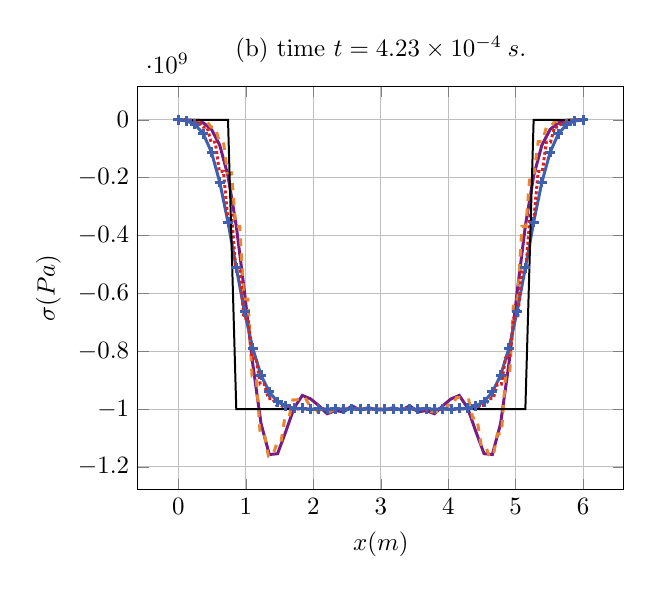
\begin{tikzpicture}[scale=0.9]
\begin{axis}[xlabel=$x (m)$,ylabel=$\sigma (Pa)$,ymajorgrids=true,xmajorgrids=true,title={(b) time $t=4.23\times 10^{-4}\: s.$}]
\addplot[Purple,very thick,mark=none,solid] coordinates {(0.0,-39934.2174897) (0.122448979592,-406302.064953) (0.244897959184,-2420460.88495) (0.367346938776,-10136844.8366) (0.489795918367,-33063216.5915) (0.612244897959,-87547121.3685) (0.734693877551,-194171704.565) (0.857142857143,-366493404.576) (0.979591836735,-596875114.898) (1.10204081633,-845116689.368) (1.22448979592,-1050481005.19) (1.34693877551,-1157297307.0) (1.4693877551,-1154376682.02) (1.59183673469,-1077374033.62) (1.71428571429,-995689036.388) (1.83673469388,-952936697.469) (1.95918367347,-964832377.273) (2.08163265306,-988568067.368) (2.20408163265,-1016260759.09) (2.32653061224,-1005179173.62) (2.44897959184,-1009892551.13) (2.57142857143,-988773783.034) (2.69387755102,-1003829596.99) (2.81632653061,-995025027.704) (2.9387755102,-1003213108.71) (3.0612244898,-1003213108.71) (3.18367346939,-995025027.704) (3.30612244898,-1003829596.99) (3.42857142857,-988773783.034) (3.55102040816,-1009892551.13) (3.67346938776,-1005179173.62) (3.79591836735,-1016260759.09) (3.91836734694,-988568067.368) (4.04081632653,-964832377.273) (4.16326530612,-952936697.469) (4.28571428571,-995689036.388) (4.40816326531,-1077374033.62) (4.5306122449,-1154376682.02) (4.65306122449,-1157297307.0) (4.77551020408,-1050481005.19) (4.89795918367,-845116689.368) (5.02040816327,-596875114.898) (5.14285714286,-366493404.576) (5.26530612245,-194171704.565) (5.38775510204,-87547121.3685) (5.51020408163,-33063216.5915) (5.63265306122,-10136844.8366) (5.75510204082,-2420460.88495) (5.87755102041,-406302.064953) (6.0,-39934.2174897) };
\addplot[Orange,very thick,mark=none,dashed] coordinates {(0.0,-10429.0753611) (0.0606060606061,-10429.0753611) (0.121212121212,-161982.808053) (0.181818181818,-161982.808053) (0.242424242424,-1267409.75703) (0.30303030303,-1267409.75703) (0.363636363636,-6575307.60772) (0.424242424242,-6575307.60772) (0.484848484848,-25213047.7874) (0.545454545455,-25213047.7874) (0.606060606061,-75630068.1866) (0.666666666667,-75630068.1866) (0.727272727273,-183565723.323) (0.787878787879,-183565723.323) (0.848484848485,-368376215.18) (0.909090909091,-368376215.18) (0.969696969697,-620238104.743) (1.0303030303,-620238104.743) (1.09090909091,-886041263.042) (1.15151515152,-886041263.042) (1.21212121212,-1086232263.3) (1.27272727273,-1086232263.3) (1.33333333333,-1162610811.08) (1.39393939394,-1162610811.08) (1.45454545455,-1121800356.23) (1.51515151515,-1121800356.23) (1.57575757576,-1031608883.18) (1.63636363636,-1031608883.18) (1.69696969697,-967968470.151) (1.75757575758,-967968470.151) (1.81818181818,-960540680.349) (1.87878787879,-960540680.349) (1.93939393939,-986227377.719) (2.0,-986227377.719) (2.06060606061,-1007602191.25) (2.12121212121,-1007602191.25) (2.18181818182,-1009726046.8) (2.24242424242,-1009726046.8) (2.30303030303,-1002072997.71) (2.36363636364,-1002072997.71) (2.42424242424,-997465464.463) (2.48484848485,-997465464.463) (2.54545454545,-998318352.653) (2.60606060606,-998318352.653) (2.66666666667,-1000280134.99) (2.72727272727,-1000280134.99) (2.78787878788,-1000550813.71) (2.84848484848,-1000550813.71) (2.90909090909,-999915604.91) (2.9696969697,-999915604.91) (3.0303030303,-999915604.91) (3.09090909091,-999915604.91) (3.15151515152,-1000550813.71) (3.21212121212,-1000550813.71) (3.27272727273,-1000280134.99) (3.33333333333,-1000280134.99) (3.39393939394,-998318352.653) (3.45454545455,-998318352.653) (3.51515151515,-997465464.463) (3.57575757576,-997465464.463) (3.63636363636,-1002072997.71) (3.69696969697,-1002072997.71) (3.75757575758,-1009726046.8) (3.81818181818,-1009726046.8) (3.87878787879,-1007602191.25) (3.93939393939,-1007602191.25) (4.0,-986227377.719) (4.06060606061,-986227377.719) (4.12121212121,-960540680.349) (4.18181818182,-960540680.349) (4.24242424242,-967968470.151) (4.30303030303,-967968470.151) (4.36363636364,-1031608883.18) (4.42424242424,-1031608883.18) (4.48484848485,-1121800356.23) (4.54545454545,-1121800356.23) (4.60606060606,-1162610811.08) (4.66666666667,-1162610811.08) (4.72727272727,-1086232263.3) (4.78787878788,-1086232263.3) (4.84848484848,-886041263.042) (4.90909090909,-886041263.042) (4.9696969697,-620238104.743) (5.0303030303,-620238104.743) (5.09090909091,-368376215.18) (5.15151515152,-368376215.18) (5.21212121212,-183565723.323) (5.27272727273,-183565723.323) (5.33333333333,-75630068.1866) (5.39393939394,-75630068.1866) (5.45454545455,-25213047.7874) (5.51515151515,-25213047.7874) (5.57575757576,-6575307.60772) (5.63636363636,-6575307.60772) (5.69696969697,-1267409.75703) (5.75757575758,-1267409.75703) (5.81818181818,-161982.808054) (5.87878787879,-161982.808054) (5.93939393939,-10429.0753609) (6.0,-10429.0753609) };
\addplot[Blue,very thick,mark=+,solid] coordinates {(0.0,-508931.478279) (0.122448979592,-3748025.68591) (0.244897959184,-16014385.4746) (0.367346938776,-47881742.3505) (0.489795918367,-112174746.169) (0.612244897959,-215592738.441) (0.734693877551,-354671855.848) (0.857142857143,-511212799.02) (0.979591836735,-663838312.129) (1.10204081633,-790213464.162) (1.22448979592,-883647482.448) (1.34693877551,-941000619.105) (1.4693877551,-974959939.111) (1.59183673469,-988927861.484) (1.71428571429,-997557909.852) (1.83673469388,-997805889.972) (1.95918367347,-1000931915.66) (2.08163265306,-998709339.041) (2.20408163265,-1001197182.01) (2.32653061224,-998859728.815) (2.44897959184,-1001017871.89) (2.57142857143,-999150004.014) (2.69387755102,-1000640138.33) (2.81632653061,-999602146.851) (2.9387755102,-1000134970.66) (3.0612244898,-1000134970.66) (3.18367346939,-999602146.851) (3.30612244898,-1000640138.33) (3.42857142857,-999150004.014) (3.55102040816,-1001017871.89) (3.67346938776,-998859728.815) (3.79591836735,-1001197182.01) (3.91836734694,-998709339.041) (4.04081632653,-1000931915.66) (4.16326530612,-997805889.972) (4.28571428571,-997557909.852) (4.40816326531,-988927861.484) (4.5306122449,-974959939.111) (4.65306122449,-941000619.105) (4.77551020408,-883647482.448) (4.89795918367,-790213464.162) (5.02040816327,-663838312.129) (5.14285714286,-511212799.02) (5.26530612245,-354671855.848) (5.38775510204,-215592738.441) (5.51020408163,-112174746.169) (5.63265306122,-47881742.3505) (5.75510204082,-16014385.4746) (5.87755102041,-3748025.68591) (6.0,-508931.478279) };
\addplot[Red,very thick,mark=none,densely dotted] coordinates {(0.0,-61223.9335744) (0.0606060606061,-61223.9335744) (0.121212121212,-884894.710625) (0.181818181818,-884894.710625) (0.242424242424,-6003361.51961) (0.30303030303,-6003361.51961) (0.363636363636,-25575128.3809) (0.424242424242,-25575128.3809) (0.484848484848,-77365275.2782) (0.545454545455,-77365275.2782) (0.606060606061,-178548645.631) (0.666666666667,-178548645.631) (0.727272727273,-330659471.659) (0.787878787879,-330659471.659) (0.848484848485,-511731335.491) (0.909090909091,-511731335.491) (0.969696969697,-686005012.829) (1.0303030303,-686005012.829) (1.09090909091,-823733433.992) (1.15151515152,-823733433.992) (1.21212121212,-914145742.521) (1.27272727273,-914145742.521) (1.33333333333,-963861687.734) (1.39393939394,-963861687.734) (1.45454545455,-986895334.229) (1.51515151515,-986895334.229) (1.57575757576,-995919063.725) (1.63636363636,-995919063.725) (1.69696969697,-998912836.991) (1.75757575758,-998912836.991) (1.81818181818,-999753499.27) (1.87878787879,-999753499.27) (1.93939393939,-999952757.55) (2.0,-999952757.55) (2.06060606061,-999992418.488) (2.12121212121,-999992418.488) (2.18181818182,-999998994.239) (2.24242424242,-999998994.239) (2.30303030303,-999999891.711) (2.36363636364,-999999891.711) (2.42424242424,-999999990.727) (2.48484848485,-999999990.727) (2.54545454545,-999999999.438) (2.60606060606,-999999999.438) (2.66666666667,-999999999.942) (2.72727272727,-999999999.942) (2.78787878788,-1000000000.02) (2.84848484848,-1000000000.02) (2.90909090909,-999999999.993) (2.9696969697,-999999999.993) (3.0303030303,-999999999.993) (3.09090909091,-999999999.993) (3.15151515152,-1000000000.02) (3.21212121212,-1000000000.02) (3.27272727273,-999999999.942) (3.33333333333,-999999999.942) (3.39393939394,-999999999.438) (3.45454545455,-999999999.438) (3.51515151515,-999999990.727) (3.57575757576,-999999990.727) (3.63636363636,-999999891.711) (3.69696969697,-999999891.711) (3.75757575758,-999998994.239) (3.81818181818,-999998994.239) (3.87878787879,-999992418.488) (3.93939393939,-999992418.488) (4.0,-999952757.55) (4.06060606061,-999952757.55) (4.12121212121,-999753499.27) (4.18181818182,-999753499.27) (4.24242424242,-998912836.991) (4.30303030303,-998912836.991) (4.36363636364,-995919063.725) (4.42424242424,-995919063.725) (4.48484848485,-986895334.229) (4.54545454545,-986895334.229) (4.60606060606,-963861687.734) (4.66666666667,-963861687.734) (4.72727272727,-914145742.521) (4.78787878788,-914145742.521) (4.84848484848,-823733433.992) (4.90909090909,-823733433.992) (4.9696969697,-686005012.829) (5.0303030303,-686005012.829) (5.09090909091,-511731335.491) (5.15151515152,-511731335.491) (5.21212121212,-330659471.659) (5.27272727273,-330659471.659) (5.33333333333,-178548645.631) (5.39393939394,-178548645.631) (5.45454545455,-77365275.2782) (5.51515151515,-77365275.2782) (5.57575757576,-25575128.3809) (5.63636363636,-25575128.3809) (5.69696969697,-6003361.51961) (5.75757575758,-6003361.51961) (5.81818181818,-884894.710625) (5.87878787879,-884894.710625) (5.93939393939,-61223.9335744) (6.0,-61223.9335744) };
\addplot[black,thick] coordinates {(0.0,-0.0) (0.122448979592,-0.0) (0.244897959184,-0.0) (0.367346938776,-0.0) (0.489795918367,-0.0) (0.612244897959,-0.0) (0.734693877551,-0.0) (0.857142857143,-1000000000.0) (0.979591836735,-1000000000.0) (1.10204081633,-1000000000.0) (1.22448979592,-1000000000.0) (1.34693877551,-1000000000.0) (1.4693877551,-1000000000.0) (1.59183673469,-1000000000.0) (1.71428571429,-1000000000.0) (1.83673469388,-1000000000.0) (1.95918367347,-1000000000.0) (2.08163265306,-1000000000.0) (2.20408163265,-1000000000.0) (2.32653061224,-1000000000.0) (2.44897959184,-1000000000.0) (2.57142857143,-1000000000.0) (2.69387755102,-1000000000.0) (2.81632653061,-1000000000.0) (2.9387755102,-1000000000.0) (3.0612244898,-1000000000.0) (3.18367346939,-1000000000.0) (3.30612244898,-1000000000.0) (3.42857142857,-1000000000.0) (3.55102040816,-1000000000.0) (3.67346938776,-1000000000.0) (3.79591836735,-1000000000.0) (3.91836734694,-1000000000.0) (4.04081632653,-1000000000.0) (4.16326530612,-1000000000.0) (4.28571428571,-1000000000.0) (4.40816326531,-1000000000.0) (4.5306122449,-1000000000.0) (4.65306122449,-1000000000.0) (4.77551020408,-1000000000.0) (4.89795918367,-1000000000.0) (5.02040816327,-1000000000.0) (5.14285714286,-1000000000.0) (5.26530612245,-0.0) (5.38775510204,-0.0) (5.51020408163,-0.0) (5.63265306122,-0.0) (5.75510204082,-0.0) (5.87755102041,-0.0) (6.0,-0.0) };
%\legend{mpm 1ppc,mpm 2ppc,modmpm 1ppc,modmpm 2ppc}
\end{axis}
\end{tikzpicture}
 \phantomsubcaption \label{subfig:mpm_diffusion_25}}\\
  {\definecolor{Purple}{RGB}{120,28,129}
\definecolor{Orange}{RGB}{231,133,50}
\definecolor{Blue}{RGB}{63,96,174}
\definecolor{Red}{RGB}{217,33,32}
\definecolor{Duck}{RGB}{83,158,182}
\definecolor{Green}{RGB}{109,179,136}
\definecolor{Yellow}{RGB}{202,184,67}
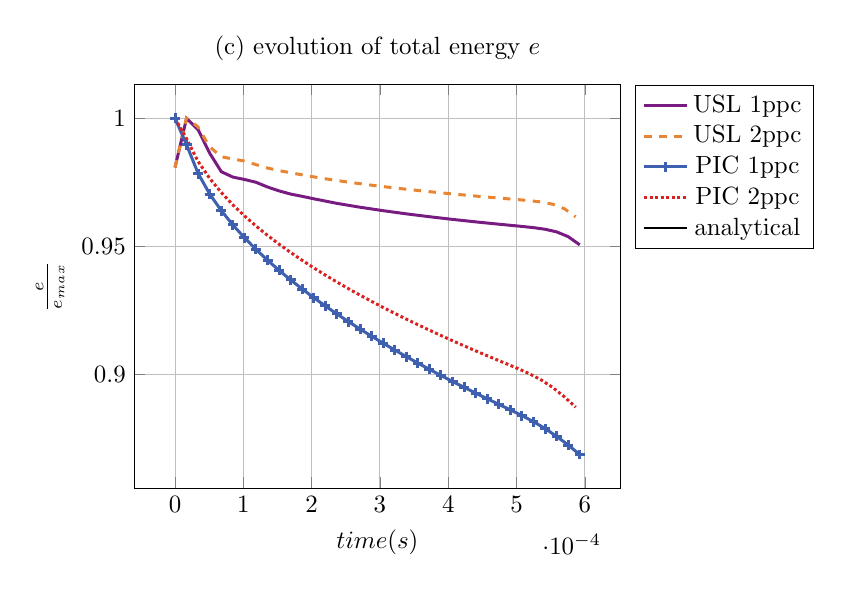
\begin{tikzpicture}[scale=0.9]
\begin{axis}[xlabel=$time (s)$,ylabel=$\frac{e}{e_{max}}$,ymajorgrids=true,xmajorgrids=true,title={(c) evolution of total energy $e$}, legend pos=outer north east]
\addplot[Purple,very thick,mark=none,solid] coordinates {(0.0,0.980776775206) (1.69272151355e-05,1.0) (3.38544302711e-05,0.995486386818) (5.07816454066e-05,0.986335480918) (6.77088605422e-05,0.979118179787) (8.46360756777e-05,0.977011836735) (0.000101563290813,0.976083552705) (0.000118490505949,0.974985958077) (0.000135417721084,0.973132007483) (0.00015234493622,0.971614043952) (0.000169272151355,0.970370597838) (0.000186199366491,0.969484052645) (0.000203126581626,0.968527091175) (0.000220053796762,0.967645365047) (0.000236981011898,0.966743210911) (0.000253908227033,0.965982183586) (0.000270835442169,0.965231974397) (0.000287762657304,0.964563191524) (0.00030468987244,0.96388114719) (0.000321617087575,0.963263530823) (0.000338544302711,0.962646353557) (0.000355471517846,0.962084695394) (0.000372398732982,0.961521764293) (0.000389325948117,0.961001071279) (0.000406253163253,0.960479919884) (0.000423180378389,0.959994795728) (0.000440107593524,0.959510651477) (0.00045703480866,0.959056403386) (0.000473962023795,0.958603029859) (0.000490889238931,0.958172736022) (0.000507816454066,0.957731808745) (0.000524743669202,0.957261239502) (0.000541670884337,0.956629022745) (0.000558598099473,0.95560284594) (0.000575525314608,0.953743784185) (0.000592452529744,0.950544066664) };
\addplot[Orange,very thick,mark=none,dashed] coordinates {(0.0,0.980776775206) (1.67562331645e-05,1.0) (3.3512466329e-05,0.996663809337) (5.02686994934e-05,0.98900666995) (6.70249326579e-05,0.985020324447) (8.37811658224e-05,0.984110580813) (0.000100537398987,0.983326915208) (0.000117293632151,0.981979184866) (0.000134049865316,0.980638155666) (0.00015080609848,0.979617302856) (0.000167562331645,0.978778886884) (0.000184318564809,0.977968446843) (0.000201074797974,0.977176694993) (0.000217831031138,0.976440965591) (0.000234587264303,0.975764557777) (0.000251343497467,0.975128766754) (0.000268099730632,0.974522184343) (0.000284855963796,0.973943735564) (0.000301612196961,0.973393220953) (0.000318368430125,0.972867749193) (0.00033512466329,0.972363947434) (0.000351880896454,0.971879647077) (0.000368637129618,0.971413467384) (0.000385393362783,0.970964070517) (0.000402149595947,0.97053007437) (0.000418905829112,0.970110254428) (0.000435662062276,0.969703595912) (0.000452418295441,0.969309210173) (0.000469174528605,0.96892621672) (0.00048593076177,0.968553101725) (0.000502686994934,0.968183689821) (0.000519443228099,0.96779053395) (0.000536199461263,0.967278784767) (0.000552955694428,0.96640240077) (0.000569711927592,0.964686590438) (0.000586468160757,0.961481917033) };
\addplot[Blue,very thick,mark=+,solid] coordinates {(0.0,1.0) (1.69272151355e-05,0.9896) (3.38544302711e-05,0.97840192) (5.07816454066e-05,0.970395814144) (6.77088605422e-05,0.963922377931) (8.46360756777e-05,0.958330092512) (0.000101563290813,0.953327939993) (0.000118490505949,0.948758714644) (0.000135417721084,0.944525461648) (0.00015234493622,0.940563061208) (0.000169272151355,0.936825160363) (0.000186199366491,0.933277336034) (0.000203126581626,0.929893178182) (0.000220053796762,0.926651891851) (0.000236981011898,0.923536752237) (0.000253908227033,0.92053406787) (0.000270835442169,0.917632461061) (0.000287762657304,0.914822354268) (0.00030468987244,0.912095594541) (0.000321617087575,0.909445173164) (0.000338544302711,0.906865012545) (0.000355471517846,0.904349801607) (0.000372398732982,0.901894866831) (0.000389325948117,0.899496069935) (0.000406253163253,0.897149725755) (0.000423180378389,0.894852535658) (0.000440107593524,0.892601494491) (0.00045703480866,0.890393110082) (0.000473962023795,0.888218874172) (0.000490889238931,0.886052220178) (0.000507816454066,0.883829497068) (0.000524743669202,0.881442958718) (0.000541670884337,0.878767030396) (0.000558598099473,0.875715616111) (0.000575525314608,0.872297097702) (0.000592452529744,0.868628627691) };
\addplot[Red,very thick,mark=none,densely dotted] coordinates {(0.0,1.0) (1.67562331645e-05,0.9921) (3.3512466329e-05,0.98321470125) (5.02686994934e-05,0.976674798128) (6.70249326579e-05,0.971199634535) (8.37811658224e-05,0.966410687731) (0.000100537398987,0.962109118378) (0.000117293632151,0.958172229577) (0.000134049865316,0.954520707917) (0.00015080609848,0.951100328411) (0.000167562331645,0.947872098186) (0.000184318564809,0.944806876372) (0.000201074797974,0.941882214857) (0.000217831031138,0.939080387869) (0.000234587264303,0.936387108509) (0.000251343497467,0.933790661554) (0.000268099730632,0.931281298637) (0.000284855963796,0.928850804847) (0.000301612196961,0.926492180888) (0.000318368430125,0.924199405234) (0.00033512466329,0.92196725296) (0.000351880896454,0.919791155586) (0.000368637129618,0.917667091102) (0.000385393362783,0.915591496621) (0.000402149595947,0.913561198187) (0.000418905829112,0.911573353815) (0.000435662062276,0.909625405615) (0.000452418295441,0.907714970883) (0.000469174528605,0.905838699657) (0.00048593076177,0.903984815557) (0.000502686994934,0.902108349787) (0.000519443228099,0.900090874846) (0.000536199461263,0.89772781162) (0.000552955694428,0.894800303924) (0.000569711927592,0.891215939989) (0.000586468160757,0.8871100207) };
\addplot[black,thick] coordinates {(0.,1.) (0.0000001,1.)};
\legend{USL 1ppc,USL 2ppc,PIC 1ppc,PIC 2ppc,analytical}
\end{axis}
\end{tikzpicture}

%%% Local Variables: 
%%% mode: latex
%%% TeX-master: "../../mainManuscript"
%%% End:
 \phantomsubcaption \label{subfig:mpm_energies}}
  \caption{Comparison USL solutions using either velocity update or interpolation and exact solution of the bars impact problem for various discretizations. (a)--(b) comparison of stress profiles at several time steps (c) evolution of total energy. Parameters: $CFL=0.7$ ; $v_0=\frac{1}{200}\sqrt{\frac{E}{\rho}}$.}
  \label{fig:mpm_diffusion}
\end{figure}

\subsection{Strategy for reducing oscillations and diffusion}
In this, we are concerned here with the accurate solution of hyperbolic problems in solid undergoing finite deformations. Although the MPM enables an efficient management of large strains, the oscillations it suffers from do not allow to accurately capture waves propagating in a medium. The above numerical results however suggest that the numerical noise can be removed by using an interpolation instead of an update of material points velocity, at the cost of additional diffusion. The point of view adopted in this thesis is that the numerical diffusion is essentially due to the projection of fields from particles to nodes and back tha spread the information. Hence, a reduction of the domain of influence of material points is preferred to a widening, as GIMP, BSMPM and DDMPM propose. 
As a consequence, a combination of the  \textit{Discontinuous Galerkin} approximation (DG) and the transfer of velocity from nodes to particles originally developed for PIC is proposed within the MPM. These two features are expected to respectively enable numerical diffusion and spurious osccilations. It is worth noticing that attention is paid to impact problems which solutions are mostly unregular so that high-order approximations, as investigated in \cite{MPM_BSpline2} or \cite{BsplineMPM}, are not considered here. 
 
% Dire un mot sur le HighOrder MPM qui n'est pas forcément désiré car on cherche à approcher des discontinuités.


%%% Local Variables: 
%%% mode: latex
%%% TeX-master: "../mainManuscript"
%%% End:


\section{Extension of the MPM to discontinuous Galerkin approximation}
\label{sec:DGMPM}
%The extension of the material point method to the DG approximation has been motivated in the previous section and is carried out hereinafter.
After a brief historical review of DG methods, the Discontinuous Galerkin Material Point Method is derived within the large strain framework with a total Lagrangian formulation. It will be seen that this new numerical approach makes use of the approximate-state Riemann solver developed in section \ref{sec:riemann_solvers} to compute intercell terms which purpose is to connect elements together. At last, the DGMPM solution scheme will be provided for hyperbolic problems.

\subsection{The discontinuous Galerkin approximation}
The DG approximation was first introduced in the context of the finite element method for the solution of the neutron transport equation \cite{NeutronDG}. This hyperbolic equation describes the advection of the angular flux which quantifies the amount of neutrons at a given location. Since neutrons can lie in a cell of a finite element mesh while its neighbors are empty, the need of describing discontinuities of the primal field across elements interfaces within a FEM context arised. Hence, an approximate solution was seeked by the Galerkin method, in a domain discretized with triangular elements by means of Lagrange polynomials that can be discontinuous across the cells. This approach amounts to duplicate the nodes of the mesh so that the support of each shape function reduces to one finite element. Those early works have launched a serie of developments of the \textbf{Discontinuous Galerkin Finite Element Method} (DGFEM) for parabolic \cite{Arnold_IPM}, elliptic \cite{Hansbo_DGsolid,Noel_HEDG}, and hyperbolic problems \cite{Cockburn}. Indeed, the DGFEM gained more and more popularity since the 80's, even for problems that do not involve discontinuities, on account of its ability to locally handle high-order approximation and its highly parallelizable nature. 
Researches conducted in the context of hyperbolic problems, of particular interest here, enabled the introduction of numerical tools developed for Finite Volume Methods (FVM) within finite element schemes.
Namely, the use of suitable \textit{slope limiters} \cite{vanLeer_Limiters} based on the \textit{total variation} \cite{Harten_TVD} enables the formulation of flexible numerical methods in which a good resolution of discontinuities is possible without destroying the accuracy in smooth regions. Furthermore, these approaches can easily handle mesh-adaption strategies by dint of the relaxation of fields continuity. Nevertheless mesh tangling problems do not vanish.
Thus, the introduction of DG approximation in the MPM should lead to a numerical method that benefits from both FEM and FVM features and enables local high-order approximation while avoiding mesh entanglement instabilities.


% %%%%%%%%%%%%%%%%%%%%%%%%%%%%%%%%%%%%%%%%%%%%%%%%%%%%%%%%%%%%%
% % Hyperbolic
% The \textit{discontinuous Galerkin (DG)} approximation enables to build numerical schemes that benefit from both finite element and finite volume methods. 
% Parler des limiteurs \cite{vanLeer_Limiters} pour atteindre la notion de schéma TVB et TVDM (TVD \cite{Harten_TVD}). Extension to RK so that the scheme can reach locally high order accuracy. In addition, the same order of accuracy is reached for velocity and gradients within a finite element framework when the weak form is based on a conservation laws system. 

% % In parallel, for parabolic or elliptic
% \cite[parabolic+penalties]{Arnold_IPM},\cite{Hansbo_DGsolid},\cite[elliptic]{Noel_HEDG}: Three field Hu-Washizu variational formulation ; assumed form of deformation gradient ; Total Lagrangian ; penalization of displacement jumps; Advantages--Drawbacks in note books

% % Introduction of HDG
% \cite{Cockburn_HDG0},\cite{Cockburn_HDG1},\cite{Cockburn_HDG2}: HDG for elliptic problems (differrence between LDG-H and HDG ?)

% % Recently extended to hyperbolic problems in solid dynamics
% \cite{NGuyen_HDG} for application to solid mechanics and extension to hyperbolic problems. Solved for displacement with enforced continuity across elements interfaces. Does not use the characteristic structure as what is done in finite volumes or original DGFEM

% However, all those approaches based on the primal field do not use the characterisitc structure. Dans l'état, ça ne peut pas être appliqué à la méca des solides puisque l'on est obligé d'imposer la continuité du champ de déplacement et donc de formuler le problème en u.
% \begin{itemize}
% \item \cite{Chavent_Salzano,Chavent_Cockburn,Cockburn_Shu,DGFEM_CFL,Cockburn}:
% \item \cite{Chavent_Salzano}--\cite{Cockburn} developments of DGFEM (mainly for fluid mechanics ?)
% \item \cite[parabolic+penalties]{Arnold_IPM},\cite{Hansbo_DGsolid},\cite[elliptic]{Noel_HEDG}: Three field Hu-Washizu variational formulation ; assumed form of deformation gradient ; Total Lagrangian ; penalization of displacement jumps; Advantages--Drawbacks in note books
% \item \cite{Cockburn_HDG0},\cite{Cockburn_HDG1},\cite{Cockburn_HDG2}: HDG for elliptic problems (differrence between LDG-H and HDG ?)
% \item \cite{NGuyen_HDG} for application to solid mechanics and extension to hyperbolic problems. Solved for displacement with enforced continuity across elements interfaces. Does not use the characteristic structure as what is done in finite volumes or original DGFEM
% \item \cite{DGPIC,DGPIC_maxwell}: application to PIC
% \end{itemize}


% RKDG - limiters - TVD - CFL - HDG (steady convection-diffusion problem (elliptic problem)) - HE DG
% Applied to steady solid mechanics problems for the ability of local high order approximation ?
% Continuity of displacement enforced through Lagrange multipliers. Benefits from superconvergence properties. A priori on utilise plus du HDG en méca du solide \cite[ALE]{NGuyen_HDG} + postprocessing pour le champ de déplacement + implicit en dynamique. Originally developed in \cite{Cockburn_HDG0}: "we may define more generally as a hybrid method any finite element method based on a formulation where one unknown is a function, or some of its derivatives, on the set $\Omega$, and the other unknown is the trace of some of its derivatives of the same function, or the trace of the function itself, along the boundaries of the set K". Numerical traces \cite{Cockburn_HDG1}


\subsection{Derivation of the DGMPM}
Consider again a continuum solid body with volume $\Omega_t$ within the time interval $\tau$. The DGMPM is expected to provide a material description of a deformation so that an approximate solution of a Lagrangian system of conservation laws written in conservative form is seeked. Recall that such a conservative form for some vector of conserved quantities $\Wcb$ reads, in Cartesian coordinates system:
\begin{equation}
  \label{eq:conservative_form}
  \drond{\Wcb}{t} + \sum_{\alpha=1}^D \drond{\Fcb\cdot \vect{e}_\alpha}{X_\alpha} = \Scb \quad \forall \vect{X},t \in \Omega_0 \times \tau
\end{equation}

\subsubsection{The DGMPM discretization}
As for MPM, a continuum body $\Omega_t$ is discretized within the time interval $\tau$ into a set of $N_p$ material points in an arbitrary Cartesian grid made of  $N_n$ nodes and $E$ non-overlapping cells of volume $\Omega^e$. The boundary of the domain is again defined by the set of edges separating empty cells from those containing particles (see figure \ref{fig:domain} for a two-dimensional example).
In addition, the reference mass density is described in the computational grid by means of the delta Dirac characteristic function and particles masses:
\begin{equation}
  \label{eq:mass_density_DGMPM}
  \rho_0\(\vect{X}\) =  \sum_{p=1}^{N_p} m_p \delta\(\vect{X}^p - \vect{X}\)
\end{equation}
where $\Omega_0$ denotes the reference configuration of the continuum. In a similar manenr to FEM and MPM, the vector of conserved quantities is approximated on the mesh by:
\begin{equation}
  \label{eq:DGMPM_node2points}
  \Wcb(\vect{X},t) = \sum^{N_n}_{i=1} S_{i}(\vect{X})\Wcb^i(t) 
\end{equation}
with $\Wcb^i$ the vector of conserved quantities at node $i$, and $S_{i}(\vect{X})$ tha shape function attached to it. Note that the convention of denoting particle and nodal fields by $p$ and $(i,j)$ still holds in this section.

\subsubsection{Weak formulation of the continuum problem}
Multiplying equation \eqref{eq:conservative_form} by a test function $\Vcb$ yields the weak formulation of the problem:
\begin{equation}
  \label{eq:weak_form}
  \begin{aligned}
    &\text{Find $\Wcb \in \Vscr_h^1$ such that} \\
    &\int_{\Omega_t} \drond{\Wcb}{t} \vect{\Vc} \: d\Omega + \int_{\Omega_t}   \drond{\Fcb_\alpha}{X_\alpha}\vect{\Vc} \: d\Omega    = \int_{\Omega_t} \Scb \vect{\Vc} \: d\Omega \quad \forall \: \vect{\Vc},t \in  \Vscr_h^1\times \tau
  \end{aligned}
\end{equation}
The key idea of DG methods is to allow jump of fields across mesh elements faces by using broken polynomial spaces for the approximate solution \cite[Ch.1]{DiPietro}:
\begin{equation}
\Vscr^k = \{ \Vcb \in H^k\Omega^e) \} \quad ;\quad \Vscr_h^k = \{\Vcb \in \Pscr^k(\Omega^e) \} \subset \Vscr^k
\end{equation}
with $H^k(\Omega^e)$, the Sobolev space and $\Pscr^k(\Omega^e)$, the space of polynomials of degree $k$ in $\Omega^e$. We restrict our attention here to linear polynomials ($k=1$). Those broken polynomials spaces allows to rewrite the weak form element-wise. After integration by part, one gets:
\begin{equation}
  \label{eq:DGMPM_weak_form}
  \begin{aligned}
    &\text{Find $\Wcb \in \Vscr_h^1$ such that} \\
    &\int_{\Omega^e} \drond{\Wcb}{t} \vect{\Vc} \: d\Omega - \int_{\Omega^e} \Fcb_\alpha  \drond{\vect{\Vc}}{X_\alpha} \: d\Omega   + \int_{\partial \Omega^e} \(\Fcb\cdot \vect{N}\)  \vect{\Vc} \: d\Gamma = \int_{\Omega^e} \Scb \vect{\Vc} \: d\Omega \quad \forall \: \vect{\Vc},e,t \in  \Vscr_h^1\times \[1,E\]\times \tau
  \end{aligned}
\end{equation}
where $\partial \Omega^e$ is the boundary of the $e$th element with outward normal vector $\vect{N}$. The dot operator $\Fcb\cdot \vect{N}$ denotes the inner product between the outward normal vector and every component of the flux, thus yielding the intercell flux, written $\Fcb_N$ for simplicity. Next, the introduction of specific fields:
\begin{equation}
  \label{eq:specific_quantities}
  \Wcb = \rho_0 \bar{\Wcb} \quad ; \quad \Fcb_\alpha = \rho_0 \bar{\Fcb}_\alpha \quad ; \quad \Scb = \rho_0 \bar{\Scb}
\end{equation}
combined with the definition of mass density \eqref{eq:mass_density_DGMPM}, leads to the following total Lagrangian formulation:
%Such a discretization of the reference mass density combined with the writing of Lagrangian conservation laws \eqref{eq:conservative_form} yields a total Lagrangian formulation, and equation \eqref{eq:DGMPM_weak_form} thus reads:
\begin{equation} 
  \label{eq:DGMPM_discrete_weak}
  \sum_{p=1}^{N_p} m_p\[\drond{\bar{\Wcb}}{t}  \vect{\Vc} - \bar{\Fcb}_{\alpha} \drond{\vect{\Vc}}{X_\alpha} -\bar{\Scb}  \vect{\Vc} \]_{|\vect{X}=\vect{X}^p} + \int_{\partial \Omega^e} \Fcb_N  \vect{\Vc} \: d\Gamma = 0 \quad \forall \: \vect{\Vc},e,t \in  \Vscr_h^1\times \[1,E\]\times \tau
\end{equation}

At last, introduction of the DGMPM approximation \eqref{eq:DGMPM_node2points} and arbitrariness of the test field in the weak form \eqref{eq:DGMPM_discrete_weak} provide the semi-discrete system that must be solved on the grid:
\begin{equation}
  \label{eq:DGMPM_semi_discrete}
  \sum_{p=1}^{N_p}\[ S_{ip} m_p S_{jp} \drond{\bar{\Wcb}^j}{t}  - \drond{S_{ip}}{X_\alpha} m_p S_{jp} \bar{\Fcb}^j_{\alpha} - S_{ip} m_p \bar{\Scb}^p\] + \int_{\Gamma_e} S_i(\vect{X}) \Fcb_N  \: d\Gamma =  0  \quad \forall \: e,t \in  \times \[1,E\]\times \tau
\end{equation}
or, in matrix form:
\begin{equation}
  \label{eq:DGMPM_semi_discrete_matrix}
  M_{ij} \drond{\bar{\Wcb}_j}{t} - K^\alpha_{ij} \bar{\Fcb}^j_{\alpha} - \Scb^i + \vect{\hat{\Fc}}^i = \vect{0}  
\end{equation}
Here again, particles plays the role of integration points in volume integrals owing to the delta Dirac characteristic function. Hence, the consistent mass matrix $M_{ij}$ may also be singular due to reduced integration so that the diagonally lumped mass matrix $M^L_i$ is used.
\begin{remark}
  \label{rq:DGPIC}
  An extension of PIC to DG approximation for the solution of Maxwell's equations is proposed in \cite{DGPIC_maxwell} and \cite{Stindl_DGPIC} in which different projections of fields between the grid and particles are used. Although those methods allow local high-order approximation, particles do not carry every fields so that the DGPIC, as the original PIC, cannot be considered as a fully Lagrangian approach. In addition, the use of Gauss quadrature rule for volume integrals of the weak form makes this approach different from that developed in the following.
\end{remark}
The discrete system is derived by discretizing the time interval $\tau$ into $N_t$ subintervals and using the explicit forward Euler method:
%Finally, the explicit forward Euler time discretization of $\tau$ in $N_t$ subinterval is perfomed, leading to the discrete system:
\begin{equation}
  \label{eq:DGMPM_discrete}
  M^L_i \frac{\bar{\Wcb}^{i,n+1} - \bar{\Wcb}^{i,n}}{\Delta t^{n} } = K^\alpha_{ij} \bar{\Fcb}_{\alpha}^{j,n} + \Scb^{i,n}- \vect{\hat{\Fc}}^{i,n}  
\end{equation}
where again, the superscripts $(\bullet)^{k,l}$ denote a field evaluated at node $k$ and time step $l$. Note that in general the source term $\Scb$ may depend on the vector of conserved quantities, hence the superscript $n$ in equation \eqref{eq:DGMPM_discrete}.
Alternatively, a \textit{second-order Runge-Kutta (RK2)} explicit time discretization may be employed, leading to the following two-stage discrete form:
\begin{equation}
  \label{eq:DGMPM_discrete_RK2}
  \begin{aligned}
    & M^L_i \frac{\bar{\Wcb}^{i,n+1/2} - \bar{\Wcb}^{i,n}}{\Delta t^{n} } = \frac{1}{2}\(K^\alpha_{ij} \bar{\Fcb}_{\alpha}^{j,n} + \Scb^{i,n}- \vect{\hat{\Fc}}^{i,n}\)  \\
    & M^L_i \frac{\bar{\Wcb}^{i,n+1} - \bar{\Wcb}^{i,n}}{\Delta t^{n} } = K^\alpha_{ij} \bar{\Fcb}_{\alpha}^{j,n+1/2} + \Scb^{i,n+1/2}- \vect{\hat{\Fc}}^{i,n+1/2}
  \end{aligned}
\end{equation}
\begin{remark}
  We chose here one existing two-stage second order Runge-Kutta method among others. See for instance \cite[Sec.~10.4.2]{Leveque} for a Total Variation Diminishing version of the RK2 time discretization. 
\end{remark}


\subsection{Non-homogeneous hyperbolic system}
Solid mechanics equations may lead to source terms in the conservative form even for neglected body forces. This is for instance the case for time-dependent plasticity (see $\Scb$ in equation \eqref{eq:vectors_elasticity}), or for cylindrical and spherical coordinates systems. In the latter situations, the gradient operators invlove terms that are not derivatives, leading to a right-hand side in system \eqref{eq:conservative_form} that depends on $\Wcb$ and called a geometric source term \cite[Ch.17]{Leveque}. Efficient procedures for the treatment of source terms $\Scb$ in non-homogeneous hyperbolic systems have been developed for finite volume methods that we propose here to take advantage of. 

A commonly used approach to solve non-homogeneous systems consists in solving alternatively a homogeneous PDEs system and a system of ODEs, namely:
\begin{subequations}
  \begin{alignat}{1}
    \label{eq:Splitting_advec} 
    & \drond{\Wcb}{t} + \sum_{\alpha=1}^D \drond{\Fcb\cdot \vect{e}_\alpha}{X_\alpha} = \vect{0}\\
    \label{eq:Splitting_ODE}
    & \ddroit{\Wcb}{t} = \Scb
  \end{alignat}
\end{subequations}
Equation \eqref{eq:Splitting_advec} is solved by applying the DGMPM discretizations \eqref{eq:DGMPM_discrete} or \eqref{eq:DGMPM_discrete_RK2}, while the solution of equation \eqref{eq:Splitting_ODE} is determined by some ODEs solver. If the discrete solution operators associated to equations \eqref{eq:Splitting_advec} and \eqref{eq:Splitting_ODE} for one time step are denoted by $H^{(\Delta t)}$ and $F^{(\Delta t)}$ respectively, the discrete solution reads \cite{Toro}:
\begin{equation}
  \label{eq:godunov_splitting}
  \Wcb^{n+1} = F^{(\Delta t)} H^{(\Delta t)} (\Wcb^n)
\end{equation}
Two sub-problems are thus solved separately at each time step, the solution of the first one being used as initial conditions in the second. \textit{Fractional-step} or \textit{Splitting} methods \eqref{eq:godunov_splitting} enable to take advantage of efficient tools already developed both for homogeneous systems of conservation laws and for ODEs. 

\begin{remark}
  The fractional-step method \eqref{eq:godunov_splitting}, known as Godunov's splitting, is only first–order accurate in time when H and F are at least first–order accurate solution operators. On the other hand, Strang splitting:
  \begin{equation}
    \label{eq:Strang_splitting}
    \Wcb^{n+1} = F^{(\Delta t/2)} H^{(\Delta t)} F^{(\Delta t/2)} (\Wcb^n)
  \end{equation}
is second-order accurate if each solution operator is at least second-order accurate \cite{Leveque}.
\end{remark}

The DGMPM solution scheme reduces to the discrete solution oparator $H^{(\Delta t)}$, or $H$ for simplicity, which in turn, aims at find approximate similarity solutions since it only solves homogeneous systems (recall remark \ref{rq:similarity_solution} in section \ref{sec:characteristic_analysis}). For a DGMPM space-time discretization made of $N_p$ material points and $N_T$ time increments, those solutions can be written:
% It has been established so far that the DGMPM scheme provides an approximate solution $\Qc(\vect{X}^i,t^{n,+1})= \Qc^{i,n+1}$,  with $i=1,...,N_n$ and $n=1,...,N_T$, that depends on the value of $\Qc$ at other points and previous time step, that is:
\begin{equation}
  \label{eq:general_scheme}
  \Qc^{p,n+1}= H \(\Qc^{j,n}\) \qquad p=1...,N_p \: ; \:j=1...,N_n \: ; \: n=0,...,N_T-1
\end{equation}
where the set of nodes $j$ having an influence on $\Qc^p$ defines the \textit{stencil} of the method. 
\begin{definition}
  \label{def:monotonicity}
  A numerical scheme is said \textbf{monotone} if it satisfies:
  \begin{equation}
    \drond{H}{\Qc^j} \geq 0 \quad \forall j
  \end{equation}
\end{definition}
The following statement then holds:
\begin{theorem}[Godunov]
  \label{th:Godunov}
  Monotone linear numerical schemes can be at most first-order accurate.
\end{theorem}


\subsection{Intercell fluxes}
\label{subsec:interface_fluxes}
Intercell fluxes of the weak form propagates information across cells by taking into account the different values that fields can take on each side of the interface. DG methods for hyperbolic problems are based on the requirement of ensuring monotonicity of the scheme for piecewise constant approximations \cite{Cockburn}. %, namely, when the discrete system identifies with a first-order finite volume scheme.  
Such a numerical method is monotone for flux functions $\Fcb_N$ that are Lipschitz continuous, consistent and monotone, namely, they must be \textit{E-fluxes} \cite{Osher}. One possibility, which is widely used and adopted here, is the \textit{Godunov flux function}. 
%The computation of interface fluxes $\hat{\Fcb}^{i,n}$ in the DGMPM system of discrete equations \eqref{eq:DGMPM_discrete} is now developed. We can here benefit from the finite volume technologies which are essentially based on the way those fluxes are computed.
\subsubsection*{The Godunov flux}
The Godunov method \cite{Godunov_method} has been proposed in the context of finite difference schemes in which the piecewise constant approximation of the solution naturally allows the definition of local Riemann problems at cells interfaces. That is, two cells $i$ and $i+1$, with interface having normal vector $\vect{N}$, define a Riemann problem in the direction $X_N=\vect{X}\cdot{N}$ which \textit{stationary solution} is used to compute the intercell numerical flux $\Fcb \cdot \vect{N}$. The stationary solution $\Wcb^*$ is the similarity solution along the vertical characteristic in the $(X_N,t)$ plane of the Riemann problem:
% Hence, the intercell numerical flux $\Fcb \cdot \vect{N}()$ is that of the stationary solution, that is, the similarity solution along the vertical straight line in the $(x,t)$ plane $\Wcb(x/t=0)$, of the Riemann problem:
\begin{equation}
  \label{eq:RP_mesh}
  \begin{aligned}
    &\drond{\Wcb}{t} + \drond{\Fcb_N}{X_N} = \vect{0}  \\
    & \Wcb(X_N,0)= \left\lbrace 
      \begin{aligned}
        & \Wcb_{X_N^-} \text{ if } X_N <0 \\
        & \Wcb_{X_N^{+}} \text{ if } X_N \geq 0
      \end{aligned}
        \right.
  \end{aligned}
\end{equation}
where $\Wcb_{X_N^-}$ and $\Wcb_{X_N^{+}}$ are the states lying infinitely close to the interface in cells $i$ and $i+1$ respectively. 
Godunov's method hence allows to account for the complete wave structure of the solution within the numerical scheme. Since this method is known to be based on E-fluxes, intercell fluxes involved in boundary integrals of weak forms of DG-methods can be computed as Godunov's ones. To this end, Riemann problems are defined at cells faces by considering that initial data are piecewise constant even for high-order approximations. Note that this strategy is also followed in FVM when high-order reconstruction techniques of the fields are used.

Let us consider as an illustration of the computation of interface fluxes within the DGMPM, the two-dimensional case depicted in figure \ref{fig:2D_edge}.
Only one Riemann problem per interface rather than nodal ones is considered in order to avoid a dramatical increase in computational time.
% Since intercell fluxes must be calculated in addition to the solution discrete equations \eqref{eq:DGMPM_discrete}, only one Riemann problem per interface is considered rather than nodal ones, in order to avoid a dramatical increase in computational time.
Thus, by averaging nodal fields on each side of the interface, one obtains mean \textit{downwind} and \textit{upwind} states $\Wcb_{X_N^-}$ and $\Wcb_{X_N^+}$ that correspond to the initial conditions of the Riemann problem.
\begin{figure}[h!]
  \centering
  \begin{tikzpicture}[scale=0.5]
  \draw (10.,0.) -- (12.,6.) ; 
  \draw[fill=black] (9.85,0.1) circle (0.1) node [left] {$1$};	
  \draw[fill=black] (10.2,-0.0) circle (0.1) node [right] {$2$};	
  \draw[fill=black] (11.85,6.1) circle (0.1) node [left] {$4$};	
  \draw[fill=black] (12.2,6) circle (0.1) node [right] {$3$};	
  \draw[->,very thick] (11.,3.) -- (12,3 -1/3) node [right,below] {$X_N$}; 
  \node at (8,3.5) {$\vect{\Qc}_{L} = \frac{\vect{\Qc}_1 + \vect{\Qc}_4}{2}$}; \node at (14.5,3.5) {$\vect{\Qc}_{R} = \frac{\vect{\Qc}_2 + \vect{\Qc}_3}{2}$};
\end{tikzpicture}

  \caption{Duplication of nodes at an interface and building of initial conditions of the Riemann problem (2D).}
  \label{fig:2D_edge}
\end{figure}
Furthermore, as mentioned in section \ref{sec:riemann_solvers}, the exact (time consuming) solution of the Riemann problem is not necessarily desired since only the stationary solution is kept. As a consequence, the stationary states are approximated here by means of an approximate-state Riemann solver, and the corresponding Godunov fluxes are determined.
\begin{remark}
  Hyperbolic systems having zero eigenvalues lead to stationary waves, propagating at zero celerity, across which the solution of the Riemann problem may have discontinuities. In that case, the associated Godunov flux is also discontinuous so that one stationary state must be considered on both sides of the characteristic. This approach leads to the computation of two fluxes, each contributing to one cell only. 
\end{remark}

Recall that hyperelasticity and elastoplasticity conservative forms (equations \eqref{eq:vectors_hyperelasticity} and \eqref{eq:vectors_plasticity}) involve strains in the vector of conserved quantities, and stresses in the flux vector.
% At last, solid mechanics conservative forms involve for hyperelasticity and elastoplasticity (equations \eqref{eq:vectors_hyperelasticity} and \eqref{eq:vectors_plasticity}), strains in the vector of conserved quantities, and stresses in the flux vector.
Hence, the calculation of Godunov's fluxes requires the integration of constitutive laws that can be time-consuming for nonlinear problems. Nevertheless, the introduction of an auxiliary vector of conserved quantities $\Qcb$ \eqref{eq:auxiliary_vectors} and the quasilinear form it provides, avoid the computation of constistutive equations. Indeed, the stationary solution of the Riemann problem is then given in terms of the auxiliary vector $\Qcb^*$, which is a rearrangement of the flux components. Thus, the generic Riemann problem solved at cells interface reads:
\begin{equation}
  \label{eq:RP_quasilinear}
  \begin{aligned}
    &\drond{\Qcb}{t} + \Jbsf \drond{\Qcb}{X_N} = \vect{0}  \\
    & \Qcb(X_N,0)= \left\lbrace 
      \begin{aligned}
        & \Qcb_{X_N^-} \text{ if } X_N <0 \\
        & \Qcb_{X_N^{+}} \text{ if } X_N \geq 0
      \end{aligned}
        \right.
  \end{aligned}
\end{equation}
with $\Qcb=\matrice{\vect{v} \\ \tens{\sigma}}$ for the infinitesimal theory and $\Qcb = \matrice{\vect{v} \\ \tens{\Pi}}$ for finite deformations. Thus, stress as well as velocity and strain must be projected back and forth between material points and nodes within the DGMPM.

\subsubsection*{Transverse corrections}

The method derived above for the computation of normal fluxes can be viewed as the \textit{Donor-Cell Upwind (DCU)} method \cite{Leveque} in which only contributions from upwind cells sharing an edge (in two dimensions) with the current one are considered. For multidimensional problems waves can travel in several directions such that contributions coming from corner cells must be taken into account in order to improve accuracy and stability of the numerical scheme. The \textit{Corner Transport Upwind (CTU)} method \cite{Colella_CTU} consists in considering contributions propagating in bias and coming from upwind cells sharing only a node (in two dimensions) with another. This approach allows to improve the Courant condition especially for solid mechanics problems for which strain components are coupled through Poisson's effect. At each cell interface, one defines left-going and right-going fluctuations as:
\begin{equation}
  \Acb^-(\Delta \Wcb) = \Fcb_N(\Wcb^*) - \Fcb_N(\Wcb_{X_N^-}) \qquad ;  \qquad \Acb^+(\Delta \Wcb) = \Fcb_N(\Wcb_{X_N^+})-\Fcb_N(\Wcb^*) 
\end{equation}
\begin{figure}[h!]
  \centering
  \definecolor{Purple}{RGB}{120,28,129}
\definecolor{Orange}{RGB}{231,133,50}
\definecolor{Blue}{RGB}{63,96,174}
\definecolor{Red}{RGB}{217,33,32}
\definecolor{Duck}{RGB}{83,158,182}
\definecolor{Green}{RGB}{109,179,136}
\definecolor{Yellow}{RGB}{202,184,67}
\begin{tikzpicture}[scale=1.8]
  \draw (0.,0.) -- (0.,2.); 
  \draw (-2.,2.) -- (2.,2.);\draw (-2.,0.) -- (2.,0.);
  \draw[->,thick,Red] (-0.25,1.4) -- (0.25,1.4) node [right] {$\Acb^{i,+}(\Delta \Wcb)$};
  \draw[->,thick,Red] (0.25,0.6) -- (-0.25,.6) node [left] {$\Acb^{i,-}(\Delta \Wcb)$};
  \node[left] at (0.,1.) {$(i)$};
  \draw[->] (0.,1.) -- (0.25,1.) node [right] {$\vect{N}^i$};
  \node[above] at (-1.5,0.)  {(k)};\node[above] at (1.5,0.)  {(m)};
  \node[below] at (-1.5,2.)  {(j)};\node[below] at (1.5,2.)  {(l)};
  \draw[->] (-0.5,0.) -- (-0.5,-0.25) node [below] {$\vect{N}^k$};
  \draw[->] (-0.5,2.) -- (-0.5,2.25) node [above] {$\vect{N}^j$};
  \draw[->] (0.5,0) -- (0.5,-0.25) node [below] {$\vect{N}^m$};
  \draw[->] (0.5,2) -- (0.5,2.25) node [above] {$\vect{N}^l$};
  \draw[->,thick,Blue] (-1.25,0.25) -- (-1.25,-0.5) node [below] {$\Bcb^{k,+} \Acb^{i,-}(\Delta \Wcb)$};
  \draw[->,thick,Blue] (-1.25,1.75) -- (-1.25,2.5) node [above] {$\Bcb^{j,+} \Acb^{i,-}(\Delta \Wcb)$};
  \draw[->,thick,Blue] (1.25,0.25) -- (1.25,-0.5) node [below] {$\Bcb^{m,+} \Acb^{i,+}(\Delta \Wcb)$};
  \draw[->,thick,Blue] (1.25,1.75) -- (1.25,2.5) node [above] {$\Bcb^{l,+} \Acb^{i,+}(\Delta \Wcb)$};
  \node[left] at (-1.,1.) {$\text{L}$} ;\node[right] at (1.,1.) {$\text{R}$} ;
  \node[above] at (-0.9,2.2) {$\text{T}$} ;
\end{tikzpicture}

%%% Local Variables: 
%%% mode: latex
%%% TeX-master: "../../mainManuscript"
%%% End:

  \caption{Normal and transverse fluctuations defined from edge $i$.}
  \label{fig:CTU}
\end{figure}
Let's consider the patch of grid cells shown in figure \ref{fig:CTU}, and focus on the edge denoted $(i)$ which local normal vector is $\vect{N}^i$. The Riemann problem defined at this edge gives rise to normal fluctuations $\Acb^{i,-}(\Delta \Wcb)$ and $\Acb^{i,+}(\Delta \Wcb)$ contributing to cells L et R respectively. These terms lead to the computation of transverse fluctuations giving contribution to neighboring cells across edges $(j)$ and $(k)$ for cell L, and across edges $(m)$ and $(l)$ for cell R. Transverse fluctuations are computed by projecting normal fluctuations onto the characteristic basis associated to the Riemann problem \eqref{eq:RP_mesh} defined on the adjacent edge, hence the name transverse Riemann solver. The spectral analysis of the corresponding Jacobian matrix, carried out in \cite{Kluth}, leads to right eigenvectors that are be written $\Rcb_{\Wc}^i$ hereinafter. The negative normal fluctuation is, for instance, decomposed on the characteristic basis associated to edge $(j)$ as:
\begin{equation}
\Acb^{i,-}(\Delta \Wcb) = \sum_{m=1}^{M} \beta_m \vect{\Rc}^{j,m}_\Wc
\end{equation}
where $\vect{\Rc}_\Wc^{j,m}$ is based on the normal vector $\vect{N}^j$ but also on different tangent moduli between grid cells L and its neighbor T. Since only waves with positive characteristic speeds with respect to the orientation defined by outward normal vector to considered edge will contribute to the transverse fluctuation, only the positive operator $\Bcb^+$ is used:
\begin{equation}
\Bcb^{j,+} \Acb^{i,-}(\Delta \Wcb) = \sum_{\underset{\lambda_m >0}{m=1}}^{M} c_m \beta_m \vect{\Rc}_\Wc^{j,m} \label{eq:transverse_fluctuations}
\end{equation}
An additional numerical flux defined at edges is hence built from these transverse fluctuations:
\begin{equation}
\Fcb^{j,\text{tran}} = \frac{\Delta t}{2 \Delta X^j} \Bcb^{j,+} \Acb^{i,-}(\Delta \Wcb) \label{eq:transverse_corrections}
\end{equation}
which contributes to the flux between cells $L$ and $T$ ($\Delta X^j$ being the length of edge $(j)$). Every corrections must be removed from intercell fluxes that can be then integrated over cells faces in order to complete the discrete system.%With duplicated nodes introduced by the DG approximation this contribution must be counted negatively for nodes belonging to cell L (outgoing fluctuation) and positively for nodes belonging to cell T (incoming fluctuation).

\begin{remark} 
  For linear elasticity, there is no need of an auxiliary vector of conserved quantity so that transverse contributions are computed with the same eigenbasis than that of the approximate-state Riemann solver.
\end{remark}

\subsubsection*{Boundary conditions enforcement}
As in MPM \cite{Love,BC_MPM}, boundary conditions (BCs) are treated at nodes that compose the domain boundary. By introducing \textit{ghost nodes} on boundary interfaces, one can widen the use of the approximate-state Riemann solver in order to enforce both Dirichlet and Neumann BCs. Similarly to finite volumes \cite{Leveque}, a state vector $\Qcb_G$ is ascribed to those nodes so that the stationary solutions of Riemann problems are consistent with boundary conditions. Dirichlet BCs enforcement for instance consists in (i) setting stress and free velocity components at ghost nodes equal to that of the associated interior node and (ii) solving the approximate Riemann problem for the velocity that must be enforced on ghost nodes knowing the stationary one that is equal to that of the BC. The same procedure holds for Neumann boundary conditions by inverting velocity and stress.
%This vector is determined for one ghost node by (i) setting the \textit{free quantities} (i.e: velocity (\textit{resp. stress}) components for Neumann (\textit{resp. Dirichlet}) BCs) equal to that of the associated interior node and (ii) solving the inverse approximate Riemann problem for \textit{enforced quantities} on ghost nodes knowing the stationary one.

Notice that the use of the auxiliary vector of conserved quantities so that state vectors contain stress %regardless of the consistutive model considered
allows to easily enforce Neumann boundary conditions. %Hence, the use of the quasi-linear form \eqref{eq:RP_quasilinear} also enables the easy treatment of boundary conditions. However, this requires that the auxiliary vector is projected onto the grid with the vector of conserved quantities.
\begin{figure}[ht]
  \centering
  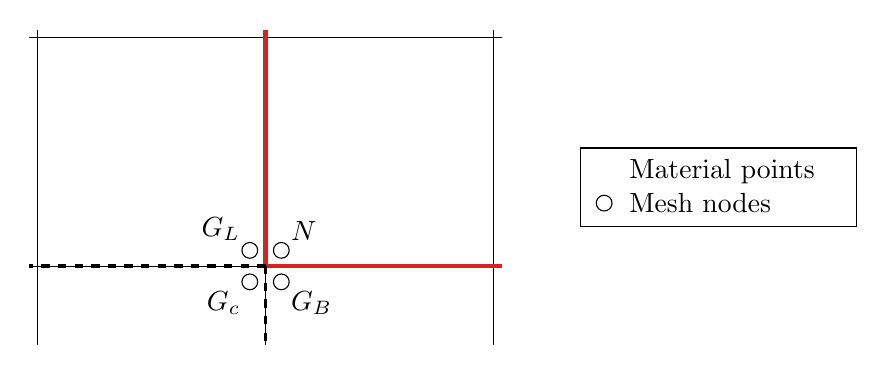
\begin{tikzpicture}
  \draw[step=2.9,black,thin] (-3.,-1.) grid (3,3.);
  \draw[ultra thick,Red] (0,3.) -- (0,0) -- (3.,0);
  % \draw[very thick,white] (0,0)--(0,-1.);
  % \draw[very thick,white] (0,0)--(-3.,-0.);
  \draw[very thick,dashed] (0,0)--(0,-1.);
  \draw[very thick,dashed] (0,0)--(-3.,-0.);
  \fill[white] (-0.2,-0.2) circle (0.1) node [below left] {$G_c$};
  \fill[white] (0.2,-0.2) circle (0.1) node [below right] {$G_B$};
  \fill[white] (-0.2,0.2) circle (0.1) node [above left] {$G_L$};
  \fill[white] (0.2,0.2) circle (0.1) node [above right] {$N$};    
  \draw[black] (-0.2,-0.2) circle (0.1) node [below left] {$G_c$};
  \draw[black] (0.2,-0.2) circle (0.1) node [below right] {$G_B$};
  \draw[black] (-0.2,0.2) circle (0.1) node [above left] {$G_L$};
  \draw[black] (0.2,0.2) circle (0.1) node [above right] {$N$};    
  \cross{0.3}{1.5};\cross{1.}{0.75};\cross{2.}{0.5};\cross{1.}{2.};
  \cross{2.5}{1.75};
  \draw (4.0,0.5) rectangle (7.5,1.5);
  \fill[white] (4.3,0.8) circle (0.1) node [right,black] {\: \text{Mesh nodes}};
  \draw[black] (4.3,0.8) circle (0.1);
  \cross{4.3}{1.2};
  \node[right] at (4.3,1.2) {\: \text{Material points}};
\end{tikzpicture}
  \caption{Corner ghost nodes in a two-dimensional DGMPM mesh.}
  \label{fig:corner_ghost}
\end{figure}
Transverse corrections further require the introduction of corner ghost nodes equivalent to finite volume corner cells \cite{Leveque}. Consider the two-dimensional case depicted in figure \ref{fig:corner_ghost} in which boundary edges are represented by red lines.
%First, boundary interfaces are extended to the corner cell (vertical and horizontal dashed lines).
First, an inverse Riemann problem is solved between the corner ghost node $G_c$ and one regular ghost node, say $G_B$, so that the stationary solution of the Riemann problem between those ghost nodes corresponds to the boundary condition holding on the vertical edge.
Second, this procedure is repeated between the corner ghost node and $G_L$ in order to enforce the boundary condition holding on the bottom boundary between them.

\begin{remark}
  \label{rq:BC_ghostnode}
  The solution of Riemann problems involving ghost nodes is made possible by extending material properties of the adjacent cell so that the characteristic structure of the solution can be computed. This implies that the deformation of interior nodes is duplicated to ghost nodes for problems such as hyperelasticity, which eigenstructure depends on the deformation gradient. Hence, for such problems ghost nodes may carry stress and strain that are not related by constitutive equations. However, the deformation gradient at ghost nodes has no physical sense and is only used to compute the correct wave speeds.
\end{remark}

\subsection{DGMPM solution scheme}
Let us assume that the vector of specific conserved quantities $\bar{\Wcb}^n$ as well as the auxiliary vector $\Qcb^n$ are known at every material points that discretize a continuum body $\Omega_0$, in a grid made of $N_{n}$ nodes at a given time $t^n$. The computational procedure followed within the DGMPM between two time steps $n$ and $n+1$ can now be derived. We consider here cases based on the use of an auxiliary vector, the others being only particular cases.
% , which requires to (i) solve the hyperbolic system \eqref{} in $\Omega$ with associated boundary conditions and (ii) update the vector $\bar{\Qcb}^n$ on material points.

The scheme has been established with a total Lagrangian formulation, therefore, the lumped mass and \textit{pseudo-stiffness} matrices $M^L_{ij}$ and $K^\alpha_{ij}$ are computed once and for all at the beginning of the calculation. The procedure then reads:
\begin{itemize}
%\item[] $\bar{\Wcb}, \:\Qcb$ known at material points
\item[(a)] The discrete equation \eqref{eq:DGMPM_discrete} and Riemann problems at cells interfaces \eqref{eq:RP_quasilinear} require a projection of fields onto the grid:
  \begin{equation}
    \label{eq:DGMPM_points2nodes}
    M^L_i \bar{\Wcb}^i = \sum_{p=1}^{N_p} S_{ip} m_p \bar{\Wcb}^p \qquad \text{and} \qquad M^L_i \vect{\Qc}^i = \sum_{p=1}^{N_p} S_{ip} m_p \vect{\Qc}^p 
  \end{equation}
  to be solved for each $\bar{\Wcb}^i$ and $\vect{\Qc}^i$ respectively. The projection of fields from particles to nodes hence follows the weighted least squares interpolation used in MPM. 
%\item[(b)] Compute time step: in the general case the tangent modulus depends on the deformation gradient as well as the waves speeds. It is therefore needed to compute the time step so that the fastest wave can at most cross the smallest cell of the mesh according to Courant condition.
\item[(b)] The specific flux vectors $\bar{\Fcb}^i_{\alpha}$ involved in the equations are computed from $\vect{\Qc}^i$ knowing $\rho_0$, thus avoiding the computation of constitutive equations.
\item[(c)] Enforcement of boundary conditions on ghost nodes.
\item[(d)] Computation of interface fluxes: 
  \begin{itemize}
  \item[1-] Build the state vectors $\vect{\Qc}_{X_N^{\pm}}$ based on $\vect{\Qc}^{i,n}$ where $i$ denotes the nodes belonging to the face on both sides of an interface.
  \item[2-] Compute the stationary solution $\Qcb^*$ by means of the approximate-state Riemann solver.
  \item[3-] Calculate the corresponding Godunov flux $\Fcb_N \(\Qcb^*\)$ by either using the DCU or the CTU approach.
  \end{itemize} 
\item[(e)] Advance solution in time by solving the discrete equation \eqref{eq:DGMPM_discrete} at each node.
\item[(f)] Back-mapping: as motivated at the end of section \ref{sec:MPM}, the nodal updated solution is projected to material points with the classical interpolation as in PIC:
  \begin{equation}
    \bar{\Wcb}^{p,n+1} = \sum_{i=1}^{N} S_{ip}\bar{\Wcb}^{i,n+1}
  \end{equation}
\item[(g)] Material point kinematics and constitutive model: The new solution $\bar{\Wcb}^{p,n+1}$ allows to increment the deformation $\vect{\varphi}(\vect{X},t)$ and to update stress components, which will be used in the auxiliary vector for the next time step, through hyperelastic constitutive equations:
  \begin{align}
    & \vect{\varphi}^{p,n+1} = \vect{X}^p + \Delta t \vect{v}^{p,n+1} \\
    & \tens{\Pi}^{p,n+1} =  \drond{\Psi}{\tens{F}}(\tens{F}^{p,n+1})
  \end{align}
  The grid may then be discarded and reconstructed and in particular by means of adaptive algorithms applied in the reference configuration, in order to improve wave front tracking in the current one.
\end{itemize}

Let's now recall or highlight significant differences between the DGMPM and the original MPM schemes. 
% Ouai ?
%First, while the DGMPM uses a classical interpolation to mapping back the updated solution to material points (step f), FLIP method and MPM require an additional time integration on material points. 
% ok
First, the use of conservation laws \eqref{eq:conservative_form} instead of the momentum equation in the weak form implies that both velocity and gradients are solved at nodes making this new approach close to finite volume methods, which provides the same order of accuracy for both fields. 
% ok
Next, since the deformation gradient is no longer calculated with shape functions gradients, the task of choosing between USF and USL algorithms vanishes. In that sense the DGMPM scheme is simpler.
At last, the solution of Riemann problems at every edges of the mesh increases computational time. Fortunately, the use of discontinuous Galerkin approximation makes this numerical method highly parallelizable \cite{Cockburn}.

The numerical scheme derived above is analyzed in terms of staiblity and convergence in the next secion.


%%% Local Variables: 
%%% mode: latex
%%% TeX-master: "../mainManuscript"
%%% End:


\section{Numerical analysis of the DGMPM}
\label{sec:DGMPM_analysis}
see Roe theorem \cite[p.417]{Toro}
\subsection{Convergence analysis}
\subsection{One-dimensional stability analysis}
Euler + RK2
\subsection{Two-dimensional stability analysis}



%%% Local Variables: 
%%% mode: latex
%%% TeX-master: "../mainManuscript"
%%% End:


\section*{Conclusion}
In this chapter, the formulation of the MPM has been recalled and some drawbacks of the method when applied to hyperbolic problems have been emphasized in section \ref{sec:MPM}. It has been seen that the projection of the nodal velocity field to material points inherited from FLIP, though it reduces the numerical diffusion, introduces noise in the solution.
Hence, an alternative method using both PIC mapping procedure and Discontinuous Galerkin approximation has been proposed in section \ref{sec:DGMPM} in order to avoid spurious oscillations.
% Hence, an alternative to this mapping procedure in order to avoid numerical dissipation within the MPM without introducing numerical noise has been proposed by means of the Discontinuous Galerkin approximation in section \ref{sec:DGMPM}.
The resulting DGMPM is based on the weak form of a system of conservation laws written element by element in an arbitrary computational grid in which particles can move. Interface fluxes involved in boundary integrals of the weak form result from the solution of Riemann problems at cells interfaces computed thanks to an approximate Riemann solver (see section \ref{subsec:interface_fluxes}). This method combines thus the strength of Finite Element and Finite Volume methods.

The numerical analysis of the scheme applied to the solution of one and two-dimensional linear scalar advection equations performed in section \ref{sec:DGMPM_analysis} led to the ability to determine the maximal Courant number ensuring stability for a given discretization.
This property allows to fully exploit the ability of the method to, for instance, rebuild the grid arbitrarily by employing adaptive mesh techniques on the reference configuration in order to accurately track waves in the current one. Indeed, after such a reconstruction, the number and positions of material points in grid cells can change and one must properly adapt the CFL number so that the scheme remains stable. An advantage on the original MPM is hence highlighted since no stability condition exists for the method. It is however worth noticing that the MPM seems less dependent to the particles distribution so that the CFL is usually set to an arbitrary value ($0.5$ or $0.7$ for one and two-dimensional problems).
The DGMPM is on the other hand, characterized by a CFL number that can be set at one in particular cases.

In addition to the stability of the method, the convergence properties of the DGMPM have been compared to that of the original MPM on a one-dimensional elastic problem. While the MPM, as FEM, shows a second-order accuracy in velocity and first-order in stress, the DGMPM exhibits a first-order accuracy for both fields. The loss of accuracy has been attributed to the back-mapping used in the DGMPM and strategies to handle higher-order approximations have been proposed. However, the purpose of this work being the accurate capturing of waves that can be non-regular, high-order accuracy goes beyond the scope of this thesis.%is not essential for it leads to more regularity in the numerical solution.

In the following, attention is paid to the capturing of waves without oscillations unlike what has been highlighted for the MPM in section \ref{sec:MPM}. The object of the next chapter is the illustration of the DGMPM performances with one and two-dimensional simulations.




%%% Local Variables: 
%%% mode: latex
%%% TeX-master: "../mainManuscript"
%%% End:
